% ============================================================
% LLM-BLM プロジェクト総合報告書
% コンパイル：tectonic LLM-BLM_総合報告書.tex   （XeTeX 系。図は LLM-BLM_総合報告書_図/ にある）
% ============================================================
\documentclass[xelatex,ja=standard,jafont=hiragino-pron,a4paper,10pt]{bxjsreport}
\setpagelayout*{left=25mm,right=25mm,top=28mm,bottom=28mm}

\usepackage{amsmath,amssymb}
\usepackage{booktabs,longtable,array,multirow}
\usepackage{graphicx}
\usepackage{xcolor}
\usepackage{tikz}
\usetikzlibrary{arrows.meta,positioning,calc,fit}
\usepackage{listings}
\usepackage{enumitem}
\usepackage{caption}
\usepackage[most]{tcolorbox}
\usepackage[hidelinks,bookmarksnumbered]{hyperref}

\graphicspath{{LLM-BLM_総合報告書_図/}}

% ---- 色
\definecolor{c1}{HTML}{2A78D6}
\definecolor{c2}{HTML}{EB6834}
\definecolor{c3}{HTML}{1BAF7A}
\definecolor{c4}{HTML}{EDA100}
\definecolor{ink2}{HTML}{52514E}
\definecolor{soft1}{HTML}{E4EEF9}
\definecolor{soft2}{HTML}{FBEEDF}
\definecolor{soft3}{HTML}{E3F3E9}
\definecolor{soft4}{HTML}{EEE8FA}
\definecolor{soft5}{HTML}{FBE6E6}

% ---- よく使う表記
\newcommand{\SP}{S\&P500}
\newcommand{\code}[1]{\texttt{#1}}
\newcommand{\term}[1]{\textsf{#1}}
\newcommand{\figref}[1]{図~\ref{#1}}
\newcommand{\tabref}[1]{表~\ref{#1}}
\newcommand{\chapref}[1]{第~\ref{#1}~章}
\newcommand{\secref}[1]{\ref{#1}~節}

% ---- リスト
\setlist[itemize]{leftmargin=1.6em,itemsep=0.2em,topsep=0.4em}
\setlist[enumerate]{leftmargin=1.8em,itemsep=0.2em,topsep=0.4em}

% ---- 表と図
\captionsetup{font=small,labelfont=bf,skip=6pt}
\renewcommand{\arraystretch}{1.25}
\setlength{\LTpre}{6pt}
\setlength{\LTpost}{6pt}

% ---- コードの表示
\renewcommand{\lstlistingname}{リスト}
\lstset{
  basicstyle=\ttfamily\scriptsize,
  breaklines=true,
  columns=fullflexible,
  keepspaces=true,
  showstringspaces=false,
  frame=single,
  framerule=0.3pt,
  rulecolor=\color{black!25},
  backgroundcolor=\color{black!3},
  xleftmargin=3pt,
  xrightmargin=3pt,
  aboveskip=8pt,
  belowskip=8pt,
  captionpos=t,
  commentstyle=\color{ink2},
  keywordstyle=\color{c1},
  stringstyle=\color{c2!80!black}
}

% ---- 要点の囲み
\newtcolorbox{keybox}[1][要点]{enhanced,breakable,colback=soft1,colframe=c1,boxrule=0.5pt,arc=2pt,
  left=8pt,right=8pt,top=6pt,bottom=6pt,title={#1},fonttitle=\sffamily\bfseries\small,coltitle=white}
\newtcolorbox{notebox}[1][注意]{enhanced,breakable,colback=soft2,colframe=c2,boxrule=0.5pt,arc=2pt,
  left=8pt,right=8pt,top=6pt,bottom=6pt,title={#1},fonttitle=\sffamily\bfseries\small,coltitle=white}

% ---- 図の部品
\tikzset{
  box/.style={draw=#1,fill=#1!12,rounded corners=2pt,align=center,inner sep=5pt,font=\small,minimum height=9mm},
  box/.default=c1,
  arr/.style={-{Stealth[length=2mm]},line width=0.6pt,color=ink2},
  lab/.style={font=\scriptsize,color=ink2}
}

\begin{document}

% ============================================================
% 表紙
% ============================================================
\hypersetup{pdftitle={LLM が生成したビューを Black-Litterman モデルに統合する手法の再現・検証・拡張},pdfauthor={小嶋 一輝},pageanchor=false}
\begin{titlepage}
\centering
\vspace*{30mm}
{\sffamily\Large 情報工学工房　プロジェクト総合報告書\par}
\vspace{14mm}
{\sffamily\bfseries\huge LLM が生成したビューを\par\vspace{3mm} Black-Litterman モデルに統合する手法の\par\vspace{3mm} 再現・検証・拡張\par}
\vspace{12mm}
{\large 概念実証（POC）、設計、実験、調査の記録\par}
\vspace{30mm}
{\large 電気通信大学　情報理工学域 III 類\par}
\vspace{3mm}
{\Large 小嶋 一輝\par}
\vspace{20mm}
{\large 2026 年 10 月 13 日 版\par}
\vfill
{\small 対象論文：Lee ほか「Integrating LLM-Generated Views into Mean-Variance Optimization Using the Black-Litterman Model」（arXiv:2504.14345）\par}
\end{titlepage}
\hypersetup{pageanchor=true}

% ============================================================
% 概要
% ============================================================
\chapter*{概要}
\addcontentsline{toc}{chapter}{概要}

本書は、大規模言語モデル（LLM）に株式の将来リターンを予想させ、その予想を Black-Litterman モデルに入れて投資比率を決める手法について、2026 年 10 月 9 日から 13 日までに行った作業をまとめたものである。対象は、Lee ほかの論文（arXiv:2504.14345）とその公式実装である。使った LLM は OpenAI の gpt-4o-mini だけで、データはすべて無料で取得できるものに限った。

作業は 4 つに分かれる。

\begin{enumerate}
\item \textbf{概念実証（POC）}：公式実装を OpenAI の API で動く形に移し、\SP{} の全構成銘柄について 30 か月分（約 44 万個）の予想を集め、元論文の計算をそのまま再現した。
\item \textbf{検証}：再現した計算を調べ、9 つの問題点を数字で確かめた。元の計算は、名前は「LLM の予想と Black-Litterman」だが、実質は「直近 1 か月に上がった銘柄を十数個選ぶ」計算になっていた。
\item \textbf{設計}：未来の情報が混ざる経路をふさぐことを中心に、データ基盤（16 のテーブルと 7 つのビュー）、月次レポートの読み取り、セクターと銘柄の指標、予測用プロンプトの入出力を設計し、大半を実装した。
\item \textbf{実験と調査}：LLM への入力と質問の形を変える 7 つの実験を行い、先行研究を調べた。
\end{enumerate}

\begin{keybox}[本書の主な結論]
\begin{itemize}
\item 元論文の計算では、Black-Litterman が市場の均衡から LLM の予想へ動かす割合が中央値で 99.9\% だった。市場の均衡はほとんど使われていない。
\item LLM の予想は、渡した月の平均リターンとの相関が平均 0.89 で、入力の値動きをなぞっている。翌月の実際のリターンとの順位相関は平均 +0.05 で、ほとんど当たっていない。
\item 元の実装の最適化は、最適な答えに届く前に止まっている。報告される比率が十数銘柄に分かれているのはそのためで、同じ式を最後まで解くと 4 銘柄前後に集中する。
\item 入力を要約した指標に変える、財務の指標を足す、考慮する比率を明言する、3 ターンの会話にする、答えを 5 段階にする、銘柄の数字を渡さずリスクプレミアムの有無を聞く、のどれを試しても、gpt-4o-mini の答えは「渡した数字の中の直近の値動き」に沿った。
\item この性質は、Chen ほか（2024）が報告した LLM の過剰な外挿と一致する。数字の処理は統計モデルに任せ、LLM には文章の解釈だけをさせる構成が、次に確かめるべき方向である。
\end{itemize}
\end{keybox}

本書の数値は、とくに断りがなければ 2026 年 10 月 10 日から 13 日の間に作ったデータベースと実験結果から計算したものである。評価期間は 30 か月しかなく、実験の多くは数百から 2,000 件程度の小さな規模である。差の大小を論じるときは、その点を前提に読んでほしい。

\setcounter{tocdepth}{1}
\tableofcontents

% ============================================================
\part{背景と目的}
% ============================================================

\chapter{はじめに}\label{ch:intro}

\section{背景}

株式の投資比率を決める古典的な方法に、平均分散最適化がある。各銘柄の期待リターンと、銘柄どうしの値動きの連動（共分散）を入力にして、リスクに対するリターンが最も良くなる比率を求める方法である。この方法には、期待リターンの見積もりが少し変わるだけで比率が大きく変わる、という弱点がある。

Black-Litterman モデルは、この弱点を和らげるために作られた。市場全体の時価総額の比率を「市場が正しいと考えている比率」とみなし、そこから逆算した期待リターンを出発点にする。そのうえで、投資家が持つ独自の見通し（ビュー）を、自信の度合いに応じて混ぜる。ビューがなければ市場の比率のままになり、ビューに自信があるほど比率が動く。

この「ビュー」は、もともと人間のアナリストが作るものだった。Lee ほかの論文は、これを LLM に作らせることを提案した。各銘柄について LLM に将来のリターンを何度も予想させ、回答の平均をビュー、回答のばらつきを自信のなさとして Black-Litterman モデルに入れる。

\section{目的}

本プロジェクトは、電気通信大学の授業「情報工学工房」の課題として、約半年をかけて次の 3 つを行うものである。本書は、その最初の 5 日間の記録である。

\begin{enumerate}
\item 対象論文の手法を、OpenAI の gpt-4o-mini だけを使って再現する。
\item 再現した手法が、主張どおりに働いているかを検証する。
\item 問題があれば、その原因を調べ、改善した手法を設計して試す。
\end{enumerate}

勝ち負け（指数を上回ったかどうか）を結論にすることは、目的にしていない。評価に使える期間は 30 か月しかなく、成績の差は偶然と区別しにくい。重視したのは、検証の確かさである。とくに、過去のデータで戦略を試すときに、その時点では知り得なかった情報が混ざらないようにすることを、設計の中心に置いた。

\section{本書の構成}

\begin{description}[leftmargin=5.5em,style=nextline,itemsep=0.3em]
\item[第 I 部　背景と目的] 理論（\chapref{ch:theory}）と、対象論文の内容（\chapref{ch:paper}）をまとめる。
\item[第 II 部　再現（POC）] 公式実装を動かすまでの経緯、作り直したシステムの構成、データ基盤、データベース、LLM による予想、比率の計算と最初の結果を述べる。
\item[第 III 部　元論文の計算の検証] 再現した計算の 9 つの問題点を、根拠の数字とともに示す。
\item[第 IV 部　拡張の設計] 未来の情報が混ざる経路の整理、月次レポートの読み取り、セクターと銘柄の指標、予測用プロンプトの入出力の設計を述べる。
\item[第 V 部　実験] 入力と質問の形を変えた 7 つの実験（A〜G）の方法と結果を述べる。
\item[第 VI 部　調査] 先行研究と、データや手法について調べたことをまとめる。
\item[第 VII 部　まとめ] 評価の観点から見た現状、残っている課題、今後の計画、結論を述べる。
\item[付録] 用語、設定の一覧、テーブル定義、スキーマの全文、プロンプトの全文、月別の数値、実験で得た回答の全文、ファイル一覧を載せる。
\end{description}

\section{主な成果}

\begin{itemize}
\item \textbf{データ基盤}：2023 年 3 月から 2026 年 9 月までの \SP{} について、各時点の構成銘柄、株価、時価総額、提出日つきの財務諸表を SQLite のデータベースにまとめた。このデータから作った時価総額加重の指数は、実際の \SP{} 指数と日次リターンの相関が 0.9997 である。
\item \textbf{再現}：各月末の構成銘柄すべて（月あたり 482〜499 銘柄）について、gpt-4o-mini に翌月のリターンを 30 個ずつ予想させた。30 か月分で 440,640 個の回答が、読み取りの失敗なしで得られた。
\item \textbf{検証}：元論文の計算を同じ式と係数で再現し、Black-Litterman がほとんど働いていないこと、予想が入力の写しであること、最適化が途中で止まっていることなど、9 つの問題点を確かめた。
\item \textbf{設計と実装}：月次レポート 39 本の読み取り、11 セクターの指標、銘柄ごとの 14 の指標を実装した。セクターの指標は、運用会社が公表しているスコアカードと照合し、モメンタムで相関 0.88〜0.96、ボラティリティで 0.97 を得た。
\item \textbf{実験}：7 つの実験で、gpt-4o-mini が渡した数字の中の「直近の値動き」に沿って答えることを、入力と質問の形を変えながら繰り返し確かめた。
\item \textbf{調査}：同じ現象を報告した先行研究（Chen ほか、2024）と、対象論文の改訂版（2025 年 10 月）の内容を確認した。
\end{itemize}

\section{現在の状態}

\begin{longtable}{p{5.20cm}p{2.00cm}p{7.20cm}}
\toprule
\textbf{項目} & \textbf{状態} & \textbf{内容} \\
\midrule
\endfirsthead
\toprule
\textbf{項目} & \textbf{状態} & \textbf{内容} \\
\midrule
\endhead
\bottomrule
\endfoot
データ基盤（株価、構成銘柄、時価総額、財務諸表） & 完了 & \chapref{ch:data}、\chapref{ch:db} \\
LLM による予想（既存手法と同じ入力） & 完了 & 30 か月、約 44 万個。\chapref{ch:views} \\
比率の計算（Black-Litterman と最適化） & 完了 & 6 つの戦略。\chapref{ch:blm} \\
元論文の計算の検証 & 完了 & 9 つの問題点。\chapref{ch:problems} \\
月次レポートの読み取り & 実装済み & 精度に問題が残る。\chapref{ch:reports}、\chapref{ch:expA} \\
セクターの指標、銘柄の指標 & 実装済み & \chapref{ch:sector}、\chapref{ch:stock} \\
予測用プロンプトの組み立て（入力の切り替え） & 設計のみ & \chapref{ch:io}。実験用のスクリプトでは動かしている \\
予想の信じ方の見直し（比率の集中への対処） & 未着手 & 案は \chapref{ch:blm} と \chapref{ch:future} \\
統計モデル（ロジスティック回帰）との比較 & 未着手 & \chapref{ch:policy} \\
結果へのフィードバックを行う LLM & 未着手 & \chapref{ch:policy} \\
\end{longtable}

\section{用語と表記}

本書でくり返し使う言葉を、ここで定めておく。くわしい用語集は付録~\ref{app:glossary} にある。

\begin{description}[leftmargin=7.5em,style=nextline,itemsep=0.2em]
\item[判断日] 投資比率を決める日。本書では、各月の最後の取引日である。判断日より後の情報は、その判断に使わない。
\item[ビュー] 投資家（ここでは LLM）が持つ、将来のリターンについての見通し。記号は $Q$。
\item[均衡リターン] 市場の時価総額の比率が最適になるような期待リターン。Black-Litterman モデルの出発点で、記号は $\Pi$。
\item[予想の不確かさ] ビューがどれだけ当てにならないかを表す分散。記号は $\Omega$。小さいほど、ビューを強く信じることになる。
\item[なぞり] LLM の予想が、渡した数字（とくに直近の値動き）とほぼ同じ向き・同じ順位になること。本書での呼び名である。
\item[実質的な銘柄数] 比率の集中の度合いを表す数。比率を $w_i$ として $1/\sum_i w_i^2$ で求める。全額を 1 銘柄に入れれば 1、$N$ 銘柄に同じ比率で入れれば $N$ になる。
\item[順位相関] 2 つの量の順位がどれだけそろうかを表す数（スピアマンの順位相関）。$-1$ から $+1$ の値を取る。
\end{description}

リターンは、とくに断らないかぎり日次の値で、小数（0.01 が $+1\%$）で扱う。本文では読みやすさのためパーセントで書くことがある。日付は \code{YYYY-MM-DD} の形で書く。ティッカー（銘柄の記号）は Yahoo Finance の書き方に合わせ、たとえば Berkshire Hathaway の B 株は \code{BRK-B} と書く。

\chapter{理論：平均分散最適化と Black-Litterman モデル}\label{ch:theory}

この章では、本書で使う計算を式で整理する。実装との対応は \chapref{ch:blm} で述べる。

\section{平均分散最適化}

銘柄の数を $N$、投資比率を $w \in \mathbb{R}^N$、期待リターンを $\mu \in \mathbb{R}^N$、共分散行列を $\Sigma \in \mathbb{R}^{N \times N}$ とする。平均分散最適化は、リターンからリスクの罰則を引いた量を最大にする比率を求める。
\begin{equation}
\max_{w}\; w^\top \mu - \frac{\delta}{2}\, w^\top \Sigma\, w
\qquad \text{条件：}\; \mathbf{1}^\top w = 1,\; w \ge 0
\label{eq:mvo}
\end{equation}
$\delta$ はリスク回避度で、大きいほどリスクを嫌う。条件は、比率の合計が 1（全額を投資する）であることと、空売りをしないことである。目的関数が 2 次式で条件が 1 次式なので、二次計画問題になる。

この方法の弱点は、$\mu$ への敏感さである。$\mu$ が少し違うだけで $w$ が大きく変わり、$\mu$ の高い少数の銘柄に比率が集中しやすい。$\mu$ を過去の平均リターンから取ると、過去にたまたま上がった銘柄に集中する。本プロジェクトでも、この性質がそのまま表れた（\chapref{ch:blm}）。

\section{Black-Litterman モデル}

\subsection{出発点：市場の均衡リターン}

Black-Litterman モデルは、$\mu$ を直接見積もらない。まず、市場全体の時価総額の比率 $w_{\mathrm{mkt}}$ が、式~\eqref{eq:mvo} の最適解になっていると仮定する。条件を外した最適化の解は $w = (\delta\Sigma)^{-1}\mu$ なので、これを逆に解くと、市場が織り込んでいる期待リターンが求まる。
\begin{equation}
\Pi = \delta\, \Sigma\, w_{\mathrm{mkt}}
\label{eq:implied}
\end{equation}
これを均衡リターンと呼び、この計算を逆最適化と呼ぶ。$\Pi$ は無リスク金利を上回る分（超過リターン）である。$\Pi$ をそのまま式~\eqref{eq:mvo} に入れれば、比率は $w_{\mathrm{mkt}}$ に戻る。

\subsection{ビューと混ぜる}

真の期待リターン $\mu$ は分からないので、確率変数として扱う。事前の見方として、$\mu$ は均衡リターンのまわりに分布すると考える。
\begin{equation}
\mu \sim \mathcal{N}(\Pi,\; \tau\Sigma)
\end{equation}
$\tau$ は均衡リターンの不確かさの大きさを決める係数である。次に、投資家のビューを $K$ 個の式で表す。
\begin{equation}
P\mu = Q + \varepsilon,\qquad \varepsilon \sim \mathcal{N}(0,\; \Omega)
\end{equation}
$P$ は $K \times N$ の行列で、どの銘柄の組み合わせについてのビューかを表す。$Q$ はビューの値、$\Omega$ はビューの不確かさである。この 2 つをベイズの定理で合わせると、事後の期待リターンが得られる。
\begin{equation}
\mu_{\mathrm{BL}} = \left[(\tau\Sigma)^{-1} + P^\top \Omega^{-1} P\right]^{-1}
\left[(\tau\Sigma)^{-1}\Pi + P^\top \Omega^{-1} Q\right]
\label{eq:bl1}
\end{equation}
同じ式は、次の形にも書ける。逆行列が 1 つで済み、$\tau\Sigma$ の逆行列を必要としない。
\begin{equation}
\mu_{\mathrm{BL}} = \Pi + \tau\Sigma P^\top \left(P\,\tau\Sigma\,P^\top + \Omega\right)^{-1}\left(Q - P\Pi\right)
\label{eq:bl2}
\end{equation}

\subsection{対象論文での形}

対象論文は、すべての銘柄について「銘柄 $i$ のリターンは $Q_i$」という絶対的なビューを置く。このとき $P$ は単位行列で、$\Omega$ は対角行列になる。式~\eqref{eq:bl2} は
\begin{equation}
\mu_{\mathrm{BL}} = \Pi + \tau\Sigma\left(\tau\Sigma + \Omega\right)^{-1}\left(Q - \Pi\right)
\label{eq:bl3}
\end{equation}
となる。銘柄が 1 つだけの場合を考えると、意味が分かりやすい。銘柄の分散を $\sigma^2$、ビューの分散を $\omega$ とすると
\begin{equation}
\mu_{\mathrm{BL}} = \Pi + \underbrace{\frac{\tau\sigma^2}{\tau\sigma^2 + \omega}}_{\text{ビューの採用率}}\,(Q - \Pi)
\label{eq:scalar}
\end{equation}
である。$\omega$ が $\tau\sigma^2$ に比べて小さければ採用率は 1 に近づき、$\mu_{\mathrm{BL}}$ はビューそのものになる。逆に $\omega$ が大きければ、均衡リターンのままになる。\textbf{ビューをどれだけ採用するかは、$\Omega$ と $\tau\Sigma$ の大きさの比で決まる。}これが、\chapref{ch:problems} で見る問題の中心である。

\begin{figure}[htbp]
\centering
\begin{tikzpicture}[node distance=7mm and 9mm]
\node[box=c3] (w) {時価総額の比率\\$w_{\mathrm{mkt}}$};
\node[box=c3,right=of w] (pi) {均衡リターン\\$\Pi=\delta\Sigma w_{\mathrm{mkt}}$};
\node[box=c4,below=12mm of w] (llm) {LLM の回答\\（30 個）};
\node[box=c4,right=of llm] (q) {ビュー $Q$（平均）\\不確かさ $\Omega$（分散）};
\node[box=c1,right=14mm of $(pi)!0.5!(q)$] (bl) {Black-Litterman\\$\mu_{\mathrm{BL}}$};
\node[box=c1,right=of bl] (opt) {最適化\\（空売りなし）};
\node[box=c2,right=of opt] (wt) {投資比率\\$w$};
\draw[arr] (w) -- node[lab,above]{逆最適化} (pi);
\draw[arr] (llm) -- node[lab,above]{集計} (q);
\draw[arr] (pi) -- (bl);
\draw[arr] (q) -- (bl);
\draw[arr] (bl) -- (opt);
\draw[arr] (opt) -- (wt);
\end{tikzpicture}
\caption{Black-Litterman モデルを使った比率の計算の流れ。共分散 $\Sigma$ は、均衡リターン、Black-Litterman、最適化の 3 か所で使う。}
\label{fig:blflow}
\end{figure}

\section{予想の不確かさ $\Omega$ の決め方}

$\Omega$ の決め方には、いくつかの流儀がある。

\begin{description}[leftmargin=2em,style=nextline,itemsep=0.3em]
\item[均衡の不確かさに合わせる（He と Litterman）] $\Omega = \mathrm{diag}(P\,\tau\Sigma\,P^\top)$ とする。ビューと均衡を同じ重みで扱うことになり、式~\eqref{eq:scalar} の採用率は 0.5 になる。
\item[自信の度合いから逆算する（Idzorek）] ビューごとに「何 \% 自信があるか」を決め、その自信に対応する $\Omega$ を逆算する。
\item[回答のばらつきを使う（対象論文）] LLM に同じ質問を何度も行い、回答の分散を $\Omega$ の対角成分にする。
\item[当たり具合から決める] 過去の予想が実際にどれだけ外れたか（予測誤差の分散）を $\Omega$ にする。
\end{description}

対象論文の方法には、注意が要る。回答の分散が表すのは「同じ質問への答えがどれだけぶれるか」であり、「予想がどれだけ外れるか」ではない。この 2 つが大きく違うと、当たらない予想を強く信じる設定になる。実際にそうなっていることを、\chapref{ch:problems} で示す。

\section{共分散の推定}

$N$ 銘柄の共分散行列を、$T$ 日分の日次リターンから計算する。標本共分散行列の階数は高々 $T-1$ なので、$T \le N$ のときは逆行列が存在しない。\SP{} は約 500 銘柄あるので、1 年分（約 252 日）でも足りない。

縮小推定は、標本共分散 $S$ を、単純な構造の行列 $F$ に寄せる方法である。
\begin{equation}
\hat{\Sigma} = (1-\alpha)\, S + \alpha\, F,\qquad 0 \le \alpha \le 1
\end{equation}
Ledoit と Wolf の方法は、寄せる強さ $\alpha$ を、推定の誤差が最小になるようにデータから決める。本プロジェクトの「直した計算」では、判断日までの 252 取引日の日次リターンにこの方法を使う。$F$ は、全銘柄の分散を平均値にそろえた対角行列である（scikit-learn の \code{LedoitWolf} の標準の設定）。

\section{評価に使う指標}

戦略の月次リターンを $r_t$（$t=1,\dots,T$）、無リスク金利を $r^f_t$、比べる相手（時価総額加重）のリターンを $b_t$ とする。

\begin{longtable}{p{3.60cm}p{5.60cm}p{5.20cm}}
\toprule
\textbf{指標} & \textbf{定義} & \textbf{意味} \\
\midrule
\endfirsthead
\toprule
\textbf{指標} & \textbf{定義} & \textbf{意味} \\
\midrule
\endhead
\bottomrule
\endfoot
年率リターン & $\bigl(\prod_t (1+r_t)\bigr)^{12/T} - 1$ & 複利で 1 年あたりに直した成績 \\
年率リスク & $\mathrm{sd}(r_t)\sqrt{12}$ & 成績のぶれの大きさ \\
シャープレシオ & $\mathrm{mean}(r_t - r^f_t)\,/\,\mathrm{sd}(r_t)\times\sqrt{12}$ & リスク 1 単位あたりの超過リターン \\
最大下落率 & 資産の最高値からの下落率の最大 & 最も苦しい時期の損失 \\
指数との差（年率） & $\mathrm{mean}(r_t - b_t)\times 12$ & 比べる相手をどれだけ上回ったか \\
指数からのずれ（年率） & $\mathrm{sd}(r_t - b_t)\sqrt{12}$ & 比べる相手からの離れ方。トラッキングエラー \\
毎月入れ替わる割合 & $\frac{1}{2}\sum_i |w_{i,t} - w_{i,t-1}|$ の平均 & 売買の量。回転率 \\
実質的な銘柄数 & $1/\sum_i w_i^2$ の平均 & 比率の集中の度合い \\
順位相関（予想と実際） & 判断日ごとに、予想の順位と翌月のリターンの順位の相関を取り、平均する & 予想がどれだけ当たっているか。情報係数（IC）とも呼ぶ \\
\end{longtable}

差が偶然かどうかの目安には、$t$ 値を使う。月ごとの差の平均を、その標準誤差（標準偏差 $/\sqrt{T}$）で割った値で、絶対値が 2 を超えると、偶然だけでは起きにくいとされる。

\section{予想の大きさを決める考え方}

LLM の出す値を、そのまま期待リターンとして使う必要はない。運用の実務では、銘柄の「点数」を期待リターンに直すとき、次の関係がよく使われる（Grinold の式）。
\begin{equation}
\alpha_i = \mathrm{IC} \times \sigma_i \times z_i
\label{eq:grinold}
\end{equation}
$z_i$ は、銘柄 $i$ の点数が銘柄全体の平均から標準偏差の何倍離れているか、$\sigma_i$ はその銘柄のリターンの標準偏差、IC は点数と実際のリターンの相関である。IC は、優れた運用者でも 0.05 前後とされる。予想がほとんど当たらないなら IC は小さく、期待リターンのずれ $\alpha_i$ も小さくなる。

この式は、\chapref{ch:blm} で見る「予想が大きすぎて比率が数銘柄に集中する」問題への、1 つの対処になる。決める係数は IC の 1 つだけで、過去のデータから測れる。本プロジェクトでは、まだ実装していない。

\chapter{対象論文とその公式実装}\label{ch:paper}

\section{論文の概要}

対象は、Lee、Kim、Kim、Lee による論文である。arXiv の番号は 2504.14345 で、2 つの版がある。

\begin{longtable}{p{2.60cm}p{5.90cm}p{5.90cm}}
\toprule
 & \textbf{第 1 版（2025 年 4 月）} & \textbf{第 2 版（2025 年 10 月）} \\
\midrule
\endfirsthead
\toprule
 & \textbf{第 1 版（2025 年 4 月）} & \textbf{第 2 版（2025 年 10 月）} \\
\midrule
\endhead
\bottomrule
\endfoot
題名 & Integrating LLM-Generated Views into Mean-Variance Optimization Using the Black-Litterman Model & LLM-Enhanced Black-Litterman Portfolio Optimization \\
発表の場 & ICLR 2025 Workshop on Financial AI & CIKM 2025 Workshop on Financial AI \\
本プロジェクトとの関係 & \textbf{再現の対象}。公式実装のコードを読んで、計算をそのまま再現した & 2026 年 10 月 13 日に内容を確認した。再現はしていない \\
\end{longtable}

手法の骨組みは、どちらの版でも同じである。

\begin{enumerate}
\item 各銘柄について、直近の日次リターンの列と会社情報（ティッカー、社名、セクター、サブ業種）を LLM に渡し、次の期間の平均日次リターンを 1 つの数値で答えさせる。
\item 同じ質問をくり返し、回答の平均をビュー $Q$、分散を不確かさ $\Omega$ とする。
\item 市場の均衡リターンとビューを Black-Litterman モデルで合わせ、平均分散最適化で比率を決める。
\end{enumerate}

\section{公式実装の構成}

公式実装は GitHub で公開されている（\code{youngandbin/LLM-BLM}）。本プロジェクトが出発点にしたのは、2025 年 10 月 21 日時点のコミット \code{1b770a9} である。処理は 7 つのスクリプトとノートブックに分かれている。

\begin{longtable}{p{0.50cm}p{5.00cm}p{9.00cm}}
\toprule
 & \textbf{ファイル} & \textbf{役割} \\
\midrule
\endfirsthead
\toprule
 & \textbf{ファイル} & \textbf{役割} \\
\midrule
\endhead
\bottomrule
\endfoot
1 & \code{run.py} & Wikipedia から構成銘柄、yfinance から株価を取り、LLM に銘柄ごとの予想を 30 回ずつ聞く。回答は月ごとの JSON に保存する \\
2 & \code{responses/}\allowbreak\code{get\_common\_stocks.py} & すべての JSON に共通して出てくる銘柄を取り出す（497 銘柄） \\
3 & \code{baselines.py} & 比べる相手（等金額、平均分散最適化）の比率と日次リターンを作る \\
4 & \code{responses\_portfolios/}\allowbreak\code{combine\_portfolio.py} & 月別の結果を 1 本につなぐ \\
5 & \code{evaluate\_multiple.py} & 本体。Black-Litterman で LLM を使った比率を計算する \\
6 & \code{calculate\_llm\_returns.py} & 5 の比率に翌月の実際のリターンを掛けて、日次リターンを出す \\
7 & \code{portfolio\_weight\_plot.ipynb} & 評価指標の計算とグラフの作成 \\
\end{longtable}

公式実装のデータは月次で区切られている。対象は 2024 年 6 月から 12 月で、評価に使えるのは 2024 年 7 月から 12 月の約 118 営業日である。LLM は Llama-3.1-8B、Gemma-7B、Qwen2-7B の 3 つで、\code{README} にある GPT の分岐はコードに実装されていなかった。

\section{時間の扱い}

公式実装のすべてのスクリプトは、「$t$ 月のデータで判断し、$t+1$ 月の実際のリターンで評価する」という決まりに従う（\figref{fig:timeline}）。本プロジェクトも、この決まりを引き継いでいる。

\begin{figure}[htbp]
\centering
\begin{tikzpicture}[x=24mm,y=9mm]
\foreach \i/\m in {0/$t-1$ 月,1/$t$ 月,2/$t+1$ 月,3/$t+2$ 月}{
  \draw[color=ink2] (\i,0) rectangle ++(1,1);
  \node[font=\small] at (\i+0.5,1.35) {\m};
}
\fill[soft4] (1,0) rectangle ++(1,1);
\fill[soft2] (2,0) rectangle ++(1,1);
\foreach \i in {0,1,2,3}{\draw[color=ink2] (\i,0) rectangle ++(1,1);}
\node[font=\small] at (1.5,0.5) {入力に使う};
\node[font=\small] at (2.5,0.5) {評価に使う};
\draw[line width=1.2pt,color=c2] (2,-0.25) -- (2,1.25);
\node[font=\small,color=c2,anchor=north] at (2,-0.3) {判断日（$t$ 月の最後の取引日）};
\end{tikzpicture}
\caption{時間の扱い。判断日より右側の情報は、その判断に使わない。}
\label{fig:timeline}
\end{figure}

\section{公式実装の計算}\label{sec:original-calc}

公式実装が行っている計算を、コードから読み取った形で書く。本プロジェクトの「元の計算」は、これをそのまま再現したものである。

\begin{description}[leftmargin=2em,style=nextline,itemsep=0.4em]
\item[事前の期待リターン] 逆最適化（式~\eqref{eq:implied}）は使わない。時価総額の比率で重み付けした市場リターン $R_m$ を作り、各銘柄のベータ $\beta_i = \mathrm{Cov}(R_i, R_m)/\mathrm{Var}(R_m)$ を求めて、$\Pi_i = \beta_i \times \mathrm{mean}(R_m - 0.02)$ とする。日次のリターンから、年率の金利 0.02 をそのまま引いている。
\item[共分散] 判断月の日次リターン（約 20 日分）の標本共分散。
\item[ビュー] $Q$ は 30 個の回答の平均、$\Omega$ は対角成分が 30 個の回答の分散、$P$ は単位行列、$\tau = 0.025$。
\item[事後の期待リターン] 式~\eqref{eq:bl1}。逆行列には、特異な行列でも計算できる疑似逆行列（\code{numpy.linalg.pinv}）を使う。
\item[最適化] $w^\top\Sigma w - 0.1\, w^\top\mu_{\mathrm{BL}}$ を最小にする。条件は比率の合計が 1、各比率が 0 以上 1 以下。解法は SciPy の \code{minimize}（SLSQP）で、設定は標準のまま、出発点は全銘柄に同じ比率である。
\item[比べる相手の平均分散最適化] 同じ目的関数で、$\mu$ を判断月の日次リターンの平均にしたもの。
\end{description}

\section{第 2 版での変更}\label{sec:v2}

第 2 版の PDF を読み、第 1 版の公式実装と違う点を確かめた。

\begin{longtable}{p{3.20cm}p{5.40cm}p{5.80cm}}
\toprule
\textbf{項目} & \textbf{第 1 版の公式実装} & \textbf{第 2 版} \\
\midrule
\endfirsthead
\toprule
\textbf{項目} & \textbf{第 1 版の公式実装} & \textbf{第 2 版} \\
\midrule
\endhead
\bottomrule
\endfoot
銘柄 & \SP{} の全体（共通の 497 銘柄） & 時価総額の上位 50 銘柄（2025 年 3 月 26 日時点） \\
期間 & 2024 年 6 月〜12 月。月ごと & 2024 年 6 月〜2025 年 6 月。2 週間ごとに見直し \\
期間の分け方 & 分けていない & 検証 3 か月（2024 年 6〜8 月）で $\tau$ を決め、テスト 10 か月（2024 年 9 月〜2025 年 6 月）で評価 \\
$\tau$ & 0.025 で固定 & 検証期間のシャープレシオで選ぶ \\
モデル & Llama、Gemma、Qwen & Gemma-7B、Qwen-2-7B、LLaMA-3.1-8B、GPT-4o-mini \\
売買のコスト & なし & 比率の変化の 0.1\% \\
比べる相手 & 等金額、平均分散最適化 & \SP{} 指数、等金額、平均分散最適化 \\
\end{longtable}

第 2 版は、結論の置き方も変えている。「どの LLM がよく当たるか」ではなく、「LLM ごとに一貫した投資スタイル（強気か弱気か、予想のばらつきの大きさ）があり、それが相場の局面に合うかどうかで成績が決まる」と述べている。

第 2 版のテスト期間の成績は、\tabref{tab:v2perf} のとおりである。gpt-4o-mini を使った Black-Litterman は、等金額を下回っている。

\begin{table}[htbp]
\centering
\caption{第 2 版が報告しているテスト期間（2024 年 9 月〜2025 年 6 月）の成績。論文の表から書き写した。}
\label{tab:v2perf}
\small
\begin{tabular}{lrrrrrr}
\toprule
 & 等金額 & 平均分散 & BL-Gemma & BL-Qwen & BL-Llama & BL-GPT \\
\midrule
年率の成長率（CAGR） & 19.1\% & 6.1\% & 15.9\% & 28.1\% & 27.5\% & 7.7\% \\
年率リスク & 19.4\% & 28.4\% & 24.8\% & 24.1\% & 19.8\% & 20.9\% \\
シャープレシオ（年率） & 0.89 & 0.28 & 0.64 & 1.06 & 1.23 & 0.36 \\
\bottomrule
\end{tabular}
\end{table}

\begin{notebox}[第 2 版について注意すること]
\begin{itemize}
\item 50 銘柄は、評価期間の途中（2025 年 3 月）の時価総額で選ばれている。評価の開始時点（2024 年 6 月）には分からなかった情報で銘柄を選んでいることになる。これは本書の指摘で、論文には書かれていない。
\item 論文は「モデルの知識の期限は評価期間より前」と述べているが、表に載っているのは各モデルの公開時期（2024 年 2〜7 月）である。
\item 論文は、予想が入力の何に沿っているかを分析していない。本書の実験（第 V 部）は、その部分を扱っている。
\end{itemize}
\end{notebox}

% ============================================================
\part{再現（概念実証）}
% ============================================================

\chapter{概念実証の経緯}\label{ch:poc}

この章では、公式実装を手元で動かし、作り直していった過程を、時間の順に述べる。

\section{公式実装を読んで分かったこと}

最初に、公式実装のコードを読み、処理の流れを整理した。そのままでは動かない箇所と、確認が必要な箇所が見つかった。

\begin{longtable}{p{2.00cm}p{4.20cm}p{8.20cm}}
\toprule
\textbf{種類} & \textbf{場所} & \textbf{内容} \\
\midrule
\endfirsthead
\toprule
\textbf{種類} & \textbf{場所} & \textbf{内容} \\
\midrule
\endhead
\bottomrule
\endfoot
動かない & \code{run.py} & API の接続先が未定義の変数（\code{\{YOUR\_API\_ENDPOINT\}}）のままで、実行できない。\code{README} にある GPT の分岐も実装されていない \\
動かない & \code{baselines.py} & 12 月の回でエラーになる。評価に使う 2025 年 1 月のデータがないため \\
要確認 & \code{evaluate\_multiple.py} & Llama と Qwen の処理がコメントになっていて、Gemma しか計算されない \\
要確認 & \code{evaluate\_multiple.py} & 均衡リターンの計算で、日次のリターンから年率の金利 0.02 をそのまま引いている \\
要確認 & ノートブック & 最大下落率に $\sqrt{252}$ を掛けている。この指標には、ふつう年率への換算をしない \\
補足 & \code{market\_caps.json} & 時価総額のファイルを作るスクリプトがなく、いつの時点の値かも分からない \\
補足 & \code{README} & 実行の順番が、実際に動く順番（5 → 6）と逆に書かれている \\
\end{longtable}

\section{OpenAI の API への移植と最初の動作確認}

2026 年 10 月 9 日に、\code{run.py} を OpenAI の API で動くように書き換え、少数のデータで動かした。出力の形は、API の構造化出力の機能で \code{\{"expected\_return": 数値\}} に固定した。

\begin{longtable}{p{3.40cm}p{11.00cm}}
\toprule
\textbf{項目} & \textbf{設定} \\
\midrule
\endfirsthead
\bottomrule
\endfoot
モデル & gpt-4o-mini \\
銘柄 & AAPL、NVDA、JPM、XOM、JNJ（セクターがばらけるように選んだ） \\
期間 & 2024 年 6 月と 7 月（6 月の予想を 7 月の実績で確かめられるように 2 か月） \\
回答の数 & 1 銘柄あたり 30 回（論文と同じ）。合計 300 回の呼び出し \\
結果 & 約 4 分で完了。300 回すべてで回答を読み取れた \\
\end{longtable}

価格データは、公式実装に含まれていたものと誤差 $10^{-6}$ 未満で一致した。予想の中身は \tabref{tab:poc5} のとおりである。

\begin{table}[htbp]
\centering
\caption{最初の動作確認の結果。6 月のデータを渡して 7 月を予想させた。値は日次の平均リターン。}
\label{tab:poc5}
\small
\begin{tabular}{lrrrrr}
\toprule
銘柄 & 入力：6 月の平均 & 予想（30 個の平均） & 予想の標準偏差 & 予想の範囲 & 7 月の実績 \\
\midrule
AAPL & $+0.48\%$ & $+0.36\%$ & 0.14\% & $+0.12\%$ 〜 $+0.72\%$ & $+0.06\%$ \\
NVDA & $+0.45\%$ & $+0.57\%$ & 0.19\% & $+0.05\%$ 〜 $+0.90\%$ & $-0.84\%$ \\
JPM & $+0.02\%$ & $+0.19\%$ & 0.08\% & $+0.03\%$ 〜 $+0.38\%$ & $+0.27\%$ \\
XOM & $+0.04\%$ & $+0.13\%$ & 0.07\% & $+0.01\%$ 〜 $+0.35\%$ & $+0.15\%$ \\
JNJ & $-0.06\%$ & $+0.08\%$ & 0.03\% & $+0.03\%$ 〜 $+0.18\%$ & $+0.49\%$ \\
\bottomrule
\end{tabular}
\end{table}

この 5 銘柄の段階で、後の検証で確かめることになる性質が、すでに見えていた。

\begin{itemize}
\item \textbf{入力をなぞっている}：予想は「先月の平均」に近い。7 月のデータを渡した回では、NVDA の先月の平均が $-0.84\%$ で、予想も $-1.08\%$ だった。
\item \textbf{プラスに偏る}：6 月時点の予想は、5 銘柄すべてプラスだった。先月がマイナスだった JNJ もプラスと予想している。
\item \textbf{大きく外すことがある}：NVDA は $+0.57\%$ の予想に対して、実績は $-0.84\%$ だった。
\end{itemize}

公式実装に含まれていた Llama-3.1-8B の回答とも比べた（\tabref{tab:llama}）。Llama の回答には、1 日 $-404\%$ のようなあり得ない値が混ざり、ばらつきが非常に大きい。対象論文は「ばらつきが大きい＝自信がない」として扱うので、モデルを替えると $\Omega$ の大きさが桁違いに変わる。

\begin{table}[htbp]
\centering
\caption{同じ銘柄・同じ月（7 月のデータから 8 月を予想）での、gpt-4o-mini と Llama-3.1-8B の比較。}
\label{tab:llama}
\small
\begin{tabular}{lrrrr}
\toprule
 & \multicolumn{2}{c}{gpt-4o-mini} & \multicolumn{2}{c}{Llama-3.1-8B（公式実装のデータ）} \\
銘柄 & 予想 & 標準偏差 & 予想 & 標準偏差 \\
\midrule
AAPL & $+0.29\%$ & 0.09\% & $-403.84\%$ & 2156.79\% \\
NVDA & $-1.08\%$ & 0.55\% & $-12.25\%$ & 69.03\% \\
JPM & $+0.39\%$ & 0.12\% & $+66.13\%$ & 418.12\% \\
XOM & $+0.26\%$ & 0.13\% & $+0.56\%$ & 0.60\% \\
JNJ & $+0.46\%$ & 0.14\% & $-41.40\%$ & 224.55\% \\
\bottomrule
\end{tabular}
\end{table}

\section{5 銘柄で Black-Litterman まで通す}

出力が後の処理に使えるかを見るため、5 銘柄の回答を公式実装の Black-Litterman の関数にそのまま渡した。ここで 2 つの問題が表に出た。

\begin{description}[leftmargin=2em,style=nextline,itemsep=0.4em]
\item[最適化が動かない] 最初の結果は、全銘柄 20.0\%（等金額と同じ）だった。最適化が 1 回で「収束した」と判断して止まり、出発点から動いていなかった。5 銘柄では目的関数の値が 0.0002 程度と小さく、SciPy の標準の停止条件（許容誤差 $10^{-6}$）にすぐ達するためである。許容誤差を $10^{-12}$ にすると、比率が動いた。
\item[均衡リターンの値がおかしい] 公式実装のとおりに計算すると、AAPL の均衡リターンが 1 日 $-1.43\%$、NVDA が $-2.94\%$ になった。日次のリターンから年率 2\% をそのまま引いているためである。日次に直した $0.02/252$ を使うと、$+0.32\%$ と $+0.67\%$ になった。
\end{description}

この 2 点は、全銘柄で確かめ直した結果、形を変えて残った。最適化は「動かない」のではなく「最適な答えに届く前に止まる」であり、均衡リターンの誤りは「結果にほとんど影響しない」ことが分かった。その理由は \chapref{ch:problems} で述べる。

\section{動作確認で見つかった問題と対処}

\begin{longtable}{p{4.00cm}p{5.40cm}p{5.00cm}}
\toprule
\textbf{問題} & \textbf{内容} & \textbf{対処} \\
\midrule
\endfirsthead
\toprule
\textbf{問題} & \textbf{内容} & \textbf{対処} \\
\midrule
\endhead
\bottomrule
\endfoot
Wikipedia の取得が失敗する & 構成銘柄の一覧の取得が HTTP 403 で失敗する。公式実装のままでは、現在は誰が実行しても動かない & User-Agent を付けて取得する \\
月末日のデータが欠ける & yfinance の終了日は「その日を含まない」ので、毎月、最後の 1 日が抜ける & 終了日を 1 日延ばして取得する \\
月の最初の日のリターンがない & 月内の株価だけで変化率を計算するので、最初の日のリターンが作れない & 前月末の終値から計算する \\
プロンプトの単位があいまい & 「percentage change」と書きながら、小数（0.0016）を渡している。モデルによっては 0.16 のように答えるおそれがある & 小数であることを明記し、例を示す \\
ティッカーの書き方 & Wikipedia の \code{BRK.B} のままでは、yfinance で株価が取れない & yfinance の書き方（\code{BRK-B}）にそろえる \\
同じ質問を 30 回送っている & 全銘柄では、1 か月分に約 7 時間かかる & 1 回のリクエストで 30 個の回答を受け取る（API の \code{n}） \\
構成銘柄が全期間で同じ & 実行した時点の一覧を、過去にさかのぼって使っている & 各月末に在籍していた銘柄を使う（\chapref{ch:data}） \\
時価総額が 1 時点の値 & いつの値か分からないファイルを、全期間に使っている & 各時点の時価総額を、株価と発行済み株式数から作る（\chapref{ch:data}） \\
\end{longtable}

\section{作り直しの履歴}

公式実装は、1 つのスクリプトにデータの取得、プロンプト、API の呼び出しが混ざっていた。これを段階的に分けていった。Git のコミットの履歴は次のとおりである。

{\footnotesize
\begin{longtable}{llp{10.50cm}}
\toprule
\textbf{コミット} & \textbf{日付} & \textbf{内容} \\
\midrule
\endfirsthead
\toprule
\textbf{コミット} & \textbf{日付} & \textbf{内容} \\
\midrule
\endhead
\bottomrule
\endfoot
\texttt{c5fab06} & 2026-10-09 & 環境構築 \\
\texttt{351c51e} & 2026-10-09 & Add .gitignore for .env, .venv and \_\_pycache\_\_ \\
\texttt{40aaa1d} & 2026-10-09 & 動作確認済み \\
\texttt{2f669bd} & 2026-10-09 & Split run.py into blm package (config / data / llm) \\
\texttt{6a2dff9} & 2026-10-10 & Read settings from .env and move file outputs to blm/output \\
\texttt{fcf3783} & 2026-10-10 & Add SQLite storage for tickers, prices and LLM views \\
\texttt{7ead68f} & 2026-10-10 & Include the last day of the month when downloading prices \\
\texttt{b7fa82a} & 2026-10-10 & Build the S\&P500 database for 2023-03 .. 2026-03 (scripts/build\_db.py) \\
\texttt{72bccb7} & 2026-10-10 & Add EDGAR financial statements and split the code into marketdb/ and llm/ \\
\texttt{6f6619f} & 2026-10-10 & Remove the original baseline / evaluation scripts and their data \\
\texttt{7600b42} & 2026-10-10 & Store LLM views in the database and ask all index members per month \\
\texttt{3b3f4f6} & 2026-10-10 & Add LLM api request timeout \\
\texttt{e488a76} & 2026-10-10 & Add portfolio construction (blm/) and run\_blm.py \\
\texttt{bdd087f} & 2026-10-13 & Add monthly report tables, sector metrics and sector ETFs \\
\texttt{ff8516b} & 2026-10-13 & run report LLM \\
\end{longtable}
}

構成の変化を、要点だけ書く。

\begin{enumerate}
\item \textbf{設定を外に出す}：実行時の引数をやめ、設定をすべて \code{.env} ファイルから読む形にした。コードの中に既定値は置かない。
\item \textbf{データをデータベースに入れる}：月ごとの CSV と JSON をやめ、SQLite のデータベース 1 つにまとめた。
\item \textbf{データと LLM を分ける}：データの取得・加工・保存を \code{marketdb/}、LLM への質問を \code{llm/} に分けた。
\item \textbf{公式実装の後半を外す}：比較用の戦略と評価のスクリプトをリポジトリから外し、比べるための写しを別のフォルダ（\code{LLM-BLM\_元コード/}）に残した。
\item \textbf{比率の計算を足す}：Black-Litterman と最適化を \code{blm/} に書いた。
\item \textbf{月次レポートと指標を足す}：\code{reports/} と、セクター・銘柄の指標の計算を足した。
\end{enumerate}

\section{全銘柄での実行}

2026 年 10 月 10 日に、全銘柄・30 か月分の予想を集めた。

\begin{longtable}{p{4.20cm}p{10.20cm}}
\toprule
\textbf{項目} & \textbf{内容} \\
\midrule
\endfirsthead
\bottomrule
\endfoot
リクエストの数 & 14,688（銘柄 $\times$ 月）。1 リクエストで 30 個の回答 \\
回答の数 & 440,640。読み取れなかった回答は 0 個 \\
費用 & 約 1.75 ドル（OpenAI の利用画面で確認した額） \\
同時に送る数 & 8 \\
起きた問題 & 1 つのリクエストが応答しないまま、約 10 分止まった。API クライアントの待ち時間の上限が標準で 600 秒だったためである。上限を 60 秒にして、失敗したリクエストを自動でやり直す設定にした \\
中断への備え & 銘柄ごとに保存し、同じ実行番号を指定すれば続きから再開できる \\
\end{longtable}

同じ質問を 30 回送る方式では、全銘柄の 1 か月分に約 7 時間かかる見込みだった。1 回で 30 個を受け取る方式にしたことで、1 か月分が数分で終わるようになった。回答はどちらの方式でも独立に生成されるので、方法として違いはない。

\chapter{システムの構成}\label{ch:system}

\section{全体像}

作り直したシステムは、4 つの入口のスクリプトと、4 つのパッケージからなる（\figref{fig:arch}）。データの流れは一方向で、すべてデータベースを通る。

\begin{figure}[htbp]
\centering
\begin{tikzpicture}[x=10mm,y=10mm]
\node[box=c3,minimum width=25mm] (src) at (0,0) {外部のデータ\\{\scriptsize Wikipedia、yfinance、EDGAR}};
\node[box=c3,minimum width=25mm] (pdf) at (0,-1.7) {月次レポート\\{\scriptsize PDF（手で集める）}};
\node[box=c1,minimum width=25mm] (mdb) at (3.7,0) {\code{marketdb/}\\{\scriptsize 取得・加工・指標}};
\node[box=c1,minimum width=25mm] (rep) at (3.7,-1.7) {\code{reports/}\\{\scriptsize レポートを読む}};
\node[box=c4,minimum width=25mm,minimum height=20mm] (db) at (7.2,-0.85) {データベース\\{\scriptsize \code{data/blm.sqlite}}\\{\scriptsize 16 テーブル、7 ビュー}};
\node[box=c1,minimum width=25mm] (llm) at (10.7,0) {\code{llm/}\\{\scriptsize 銘柄の予想を集める}};
\node[box=c1,minimum width=25mm] (blm) at (10.7,-1.7) {\code{blm/}\\{\scriptsize 比率を計算する}};
\node[box=c2,minimum width=25mm] (api) at (7.2,-3.3) {OpenAI の API\\{\scriptsize gpt-4o-mini}};
\draw[arr] (src) -- (mdb);
\draw[arr] (pdf) -- (rep);
\draw[arr] (mdb.east) -- (db.west|-mdb.east);
\draw[arr] (rep.east) -- (db.west|-rep.east);
\draw[arr,{Stealth[length=2mm]}-{Stealth[length=2mm]}] (db.east|-llm.west) -- (llm.west);
\draw[arr,{Stealth[length=2mm]}-{Stealth[length=2mm]}] (db.east|-blm.west) -- (blm.west);
\draw[arr,dashed] (rep.south) |- (api.west);
\draw[arr,dashed] (llm.east) -- ++(0.4,0) |- (api.east);
\end{tikzpicture}
\caption{システムの全体像。実線はデータの流れ、破線は API の呼び出しを表す。\code{llm/} と \code{blm/} は、データベースを通してだけつながる。}
\label{fig:arch}
\end{figure}

\section{ファイルの一覧}

Python のコードは合計で約 2,200 行である。各ファイルの役割は次のとおりで、表の説明はファイルの冒頭に書いてある説明文をそのまま載せている。

{\footnotesize
\begin{longtable}{p{5.20cm}rp{8.20cm}}
\toprule
\textbf{ファイル} & \textbf{行数} & \textbf{役割（ファイル冒頭の説明）} \\
\midrule
\endfirsthead
\toprule
\textbf{ファイル} & \textbf{行数} & \textbf{役割（ファイル冒頭の説明）} \\
\midrule
\endhead
\bottomrule
\endfoot
\texttt{blm/black\_\allowbreak{}litterman.py} & 25 & Black-Litterman posterior returns with one absolute view per stock (P = identity). \\
\texttt{blm/config.py} & 34 & Settings of the portfolio calculation (read from LLM-BLM/.env, every value is expected to be set there). \\
\texttt{blm/covariance.py} & 16 & Covariance of daily returns. \\
\texttt{blm/equilibrium.py} & 16 & Market equilibrium returns (the prior of Black-Litterman). \\
\texttt{blm/evaluation.py} & 38 & Performance figures from monthly returns. \\
\texttt{blm/inputs.py} & 56 & Everything the strategies need for one decision date, read from the database. \\
\texttt{blm/optimizer.py} & 38 & Long-only, fully invested mean-variance optimization. \\
\texttt{blm/strategies.py} & 70 & Strategies: each one takes the inputs of a decision date and returns the weights of the universe. \\
\texttt{llm/client.py} & 52 & OpenAI API calls with structured output. \\
\texttt{llm/config.py} & 37 & Settings of the LLM run: API / model / sampling, months and tickers \\
\texttt{llm/context.py} & 14 & Information passed to the LLM for each ticker. \\
\texttt{llm/prompts.py} & 36 & Prompts for predicting the next month's average daily return. \\
\texttt{llm/returns.py} & 21 & Months to process and daily returns given to the LLM. \\
\texttt{marketdb/build\_\allowbreak{}db.py} & 260 & Build the SQLite database for the study period (DB\_START\_DATE .. DB\_END\_DATE in .env). \\
\texttt{marketdb/\allowbreak{}build\_\allowbreak{}fundamentals.\allowbreak{}py} & 129 & Fetch financial statements of every S\&P500 member in the database from SEC EDGAR. \\
\texttt{marketdb/\allowbreak{}build\_\allowbreak{}sector\_\allowbreak{}metrics.\allowbreak{}py} & 43 & Compute the sector indicators for the last trading day of every month and store them in sector\_metrics. \\
\texttt{marketdb/\allowbreak{}build\_\allowbreak{}stock\_\allowbreak{}metrics.\allowbreak{}py} & 43 & Compute the stock indicators of the index members for the last trading day of every month \\
\texttt{marketdb/config.py} & 38 & Settings of the market database: data sources, database file and stored period \\
\texttt{marketdb/db/connection.py} & 22 & SQLite connection and table creation. \\
\texttt{marketdb/db/fundamentals.py} & 34 & Save financial statement values (financial\_items / financial\_facts). \\
\texttt{marketdb/db/index.py} & 38 & Save / load S\&P500 constituent changes and membership periods. \\
\texttt{marketdb/db/llm.py} & 55 & Save / load LLM runs and answers (llm\_runs / llm\_views). \\
\texttt{marketdb/db/market.py} & 117 & Save / load tickers and daily close prices. \\
\texttt{marketdb/db/portfolio.py} & 37 & Save / load portfolios (portfolio\_runs / portfolio\_weights). \\
\texttt{marketdb/db/reports.py} & 86 & Save / load monthly reports and their analyses (reports / report\_runs / report\_values). \\
\texttt{marketdb/db/sector.py} & 56 & Save / load sector indicators (sector\_metrics). \\
\texttt{marketdb/db/stock.py} & 34 & Save / load stock indicators (stock\_metrics). \\
\texttt{marketdb/sources/edgar.py} & 76 & Financial statements from SEC EDGAR (XBRL company facts) and company id (CIK) lookup. \\
\texttt{marketdb/sources/prices.py} & 18 & Daily price download (yfinance). \\
\texttt{marketdb/sources/shares.py} & 23 & Shares outstanding and split history from yfinance. \\
\texttt{marketdb/sources/universe.py} & 58 & S\&P500 constituents (ticker, company name, GICS sector / sub-industry) and their change history. \\
\texttt{marketdb/\allowbreak{}transform/\allowbreak{}membership.\allowbreak{}py} & 40 & Rebuild S\&P500 membership periods from the current constituents and the change history. \\
\texttt{marketdb/transform/sector.py} & 66 & Sector indicators on a decision date: momentum and volatility from the sector ETF, \\
\texttt{marketdb/transform/shares.py} & 32 & Shares outstanding converted to the current split basis. \\
\texttt{marketdb/transform/stock.py} & 105 & Stock indicators on a decision date: price behaviour from daily prices, \\
\texttt{reports/client.py} & 33 & OpenAI API call that reads one report (the PDF pages are sent as they are, so charts and tables are seen too). \\
\texttt{reports/config.py} & 33 & Settings of the report analysis: API / model, report folder, reports to analyse \\
\texttt{reports/items.py} & 48 & Items read from a monthly report. Change this list to change what the LLM returns: \\
\texttt{reports/loader.py} & 45 & Find the report files in data/reports and read what is registered in the database. \\
\texttt{reports/prompts.py} & 35 & Prompt and answer format for reading a monthly report, built from reports/items.py. \\
\texttt{run\_\allowbreak{}blm.py} & 35 & Compute portfolio weights for every decision date of an LLM run and store them in the database. \\
\texttt{run\_\allowbreak{}llm.py} & 88 & Collect LLM views (expected returns) for S\&P500 stocks and store them in the database. \\
\texttt{run\_\allowbreak{}reports.py} & 62 & Register the monthly reports in data/reports and read them with the LLM; the answers are stored in the database. \\
\end{longtable}
}

\section{依存の向き}

パッケージの間の依存は、一方向に限っている。

\begin{itemize}
\item \code{llm/}、\code{blm/}、\code{reports/} は、\code{marketdb/} の関数を使ってデータベースを読み書きする。
\item \code{llm/}、\code{blm/}、\code{reports/} は、互いを使わない。たとえば \code{blm/} は、LLM の回答をデータベースから読むだけで、\code{llm/} のコードを呼ばない。
\item \code{marketdb/} は、ほかの 3 つを使わない。
\end{itemize}

こうしておくと、予想の集め方を変えても比率の計算に手を入れずに済み、逆も同じである。実験のたびに条件を変えて比べる作業では、この分け方が効く。

\section{設定}

設定は、すべてリポジトリ直下の \code{.env} ファイルに書く。次の決まりにしている。

\begin{itemize}
\item 実行時の引数は使わない。スクリプトは \code{python run\_llm.py} のように、何も付けずに実行する。
\item コードの中に既定値を置かない。設定が欠けていれば、起動時にエラーで止まる。
\item 係数（$\tau$、リスク回避度など）も \code{.env} に置く。実際に使った値は、結果と一緒にデータベースにも保存する。
\item API キーが入っているので、\code{.env} は Git に入れない。代わりに、キーを空にした \code{.env.example} を入れている。
\end{itemize}

設定の一覧は、付録~\ref{app:env} にある。

\section{実行の手順}

\begin{lstlisting}[language=bash]
python -m venv .venv
.venv/bin/pip install -r requirements.txt
cp .env.example .env                      # OPENAI_API_KEY を入れる

python marketdb/build_db.py               # 株価・構成銘柄・株式数・ETF をデータベースに入れる
python marketdb/build_fundamentals.py     # 財務諸表を入れる
python marketdb/build_sector_metrics.py   # セクターの指標を計算する
python marketdb/build_stock_metrics.py    # 銘柄の指標を計算する
python run_llm.py                         # LLM に銘柄ごとの予想を聞く
python run_blm.py                         # 比率を計算する
python run_reports.py                     # 月次レポートを LLM に読ませる
\end{lstlisting}

どのスクリプトも、途中で止まっても再実行できる。データの取得は、すでに入っているテーブルを飛ばす。LLM の実行は、回答済みの銘柄やレポートを飛ばす。

\section{再現性のための仕組み}

LLM の回答は乱数で生成されるので、同じ設定でも実行のたびに変わる。そのため、「同じ数字をもう一度出せる」ことではなく、「保存した回答から同じ結果を計算し直せる」ことを、再現性の意味としている。

\begin{description}[leftmargin=2em,style=nextline,itemsep=0.4em]
\item[実行ごとに条件を残す] LLM の実行（\code{llm\_runs}）、レポートの読み取り（\code{report\_runs}）、比率の計算（\code{portfolio\_runs}）は、それぞれ 1 回の実行が 1 行になる。モデルの版、プロンプトの全文、回答の数、係数を保存する。
\item[結果を加工せずに残す] 平均と分散だけでなく、30 個の回答をすべて保存する。後から別の集計ができる。
\item[違う設定を混ぜない] 実行番号を指定して続きから動かすとき、モデル、プロンプト、回答の数などが保存済みの値と違えば、書き込まずに止まる。
\item[データは 1 回取って固定する] 配当や株式分割で調整した株価は、取得する時期によって過去の分まで変わる。全期間を 1 回で取得し、その後は上書きしない。
\end{description}

データベースのファイル（約 200 MB）は Git に入れていない。別の環境で作業するときは、ファイルをそのまま渡すか、上の手順で作り直す。作り直した場合、株価の調整後の値と LLM の回答は、元と同じにはならない。

\chapter{データ基盤}\label{ch:data}

この章では、データをどこから取り、どう加工し、何を除外したかを述べる。あわせて、実際の \SP{} と違う点を整理する。

\begin{keybox}
\begin{itemize}
\item 期間は 2023-03-01 から 2026-09-30 の 900 営業日。取得日は 2026 年 10 月 10 日である。
\item 期間中に在籍した 568 銘柄のうち、データが取れない 28 銘柄を除外し、540 銘柄を使う。
\item このデータから作った時価総額加重の指数は、実際の \SP{} 指数と日次リターンの相関が 0.9997 で、期間全体の騰落率は $+94.1\%$ と $+93.6\%$ である。
\item 公式のデータではなく、無料で取れるデータによる近似である。構成比率は浮動株で調整しておらず、除外した銘柄による生存者バイアスがある。
\end{itemize}
\end{keybox}

\section{データの出どころ}

\begin{longtable}{p{3.60cm}p{4.60cm}p{6.20cm}}
\toprule
\textbf{データ} & \textbf{取得元} & \textbf{注意} \\
\midrule
\endfirsthead
\toprule
\textbf{データ} & \textbf{取得元} & \textbf{注意} \\
\midrule
\endhead
\bottomrule
\endfoot
現在の構成銘柄、社名、業種の分類 & Wikipedia「List of S\&P 500 companies」 & 取得時点（2026 年 10 月）の内容。誰でも編集できるページである \\
指数から外れた銘柄の業種 & 同じページの過去の版 & 四半期の初日ごとの版を新しい順に見て、外れる直前の分類を入れる \\
銘柄の入れ替えの履歴 & Wikipedia「Historical components of the S\&P 500」 & 1976 年からの 412 件。期間中は 74 件 \\
日次の株価 & yfinance（Yahoo Finance） & 取得日の基準で調整済み。上場廃止の銘柄は取れない \\
発行済み株式数 & yfinance & 報告日だけの不定期な値。揺れや欠けがある \\
\SP{} 指数 & yfinance（\code{\textasciicircum GSPC}） & 配当を含まない価格指数 \\
無リスク金利 & yfinance（\code{\textasciicircum IRX}） & 3 か月物の米国債の利回り。年率のパーセント \\
セクター別の ETF（11 本） & yfinance（XLK、XLF など） & セクターの指標の計算に使う。2023 年 1 月から \\
予想変動率などの指数 & yfinance（\code{\textasciicircum VIX}、\code{\textasciicircum VIX3M}、\code{\textasciicircum SKEW}） & 市場全体の状態を表す \\
財務諸表 & 米国証券取引委員会の EDGAR（XBRL company facts） & 提出日つき。最初に提出された値を保存する \\
月次レポート & 大和アセットマネジメントの月次の見通し（PDF） & 手で集めた 39 本。\chapref{ch:reports} \\
\end{longtable}

\SP{} を算出している会社の公式データ（構成銘柄、浮動株、構成比率）は有料なので、使っていない。

\section{株価と株式分割の扱い}

yfinance の値は、種類によって調整の有無が違う。終値と調整後終値は株式分割で調整されているが、発行済み株式数は報告されたままの値である。そのまま掛け算すると、分割の前後で時価総額が食い違う。

NVIDIA は 2024 年 6 月 10 日に、1 株を 10 株に分割した。分割前の 6 月 6 日について、yfinance の終値は 121.00 ドル（当時の実際の株価は約 1,210 ドル）、株式数は 24.6 億株（分割後の基準では 246 億株）である。これを掛けると約 0.3 兆ドルになり、実際の約 3 兆ドルの 10 分の 1 になる。

\textbf{対処として、データベースに入れる前に、株式数を取得日の分割の基準に直す。}株価はもともと今の基準なので、株式数のほうを合わせる。これで、時価総額は「終値 $\times$ 株式数」の掛け算だけで求まる。取り込むときの処理は 3 つである。

\begin{enumerate}
\item \textbf{今の基準に直す}：報告日より後に行われた分割の比率を、報告値に掛ける。
\item \textbf{外れ値を捨てる}：前後 30 日の値の中央値と比べて、2 倍以上または半分以下の値を捨てる。分割日の前なのに、すでに分割後の値で報告されている行があるためである。NVIDIA では 2024-06-08 の報告がこれに当たり、単純に 10 倍すると時価総額が 10 倍ずれていた。
\item \textbf{1 日 1 つにする}：同じ日に複数の報告があれば、中央値を使う。
\end{enumerate}

リターンの計算には、配当を含む調整後終値を使う。時価総額の計算には、配当で調整していない終値を使う。調整後終値を使うと、配当の多い銘柄ほど過去の時価総額が小さく出るためである。

\section{時価総額と構成比率}

構成比率が必要なのは、Black-Litterman の出発点（均衡リターン）を作るところだけである。次の式で作る。
\[
\text{構成比率} = \frac{\text{その銘柄の時価総額}}{\text{その日に在籍している銘柄の時価総額の合計}},\qquad
\text{時価総額} = \text{終値} \times \text{発行済み株式数}
\]

浮動株（市場で実際に取引できる株）による調整はしていない。yfinance の浮動株数は今日の値しか取れず、種類株のある会社では値が壊れ（Alphabet では 100\% を超える）、上場廃止の銘柄では取れないためである。

種類株のある 3 社（Alphabet、Fox、News Corp）については、yfinance がどの種類にも会社全体の株式数を返す。そのままでは会社が二重に数えられるので、現在の種類ごとの株式数の比率で振り分けている。

\section{各時点の構成銘柄}

Wikipedia の構成銘柄の一覧は「今の」\SP{} である。期間中に 74 件の入れ替えがあり、今の一覧で過去を検証すると、2 つの偏りが入る。

\begin{itemize}
\item \textbf{生存者バイアス}：途中で外れた銘柄（破綻、買収、時価総額の減少）が、最初から入っていないことになる。
\item \textbf{先読みバイアス}：後から株価が上がって指数に採用された銘柄を、採用される前から持つことになる。
\end{itemize}

これを避けるため、今の構成銘柄から入れ替えの履歴を新しい順に取り消していき、銘柄ごとの在籍期間を再現した。在籍期間は「開始日」と「終了日」の組で持ち、ある日の構成銘柄は 1 つの SQL で取り出せる。

\begin{lstlisting}[language=SQL]
SELECT symbol FROM index_membership
WHERE (start_date IS NULL OR start_date <= '2024-06-03')
  AND (end_date   IS NULL OR end_date   >  '2024-06-03');
\end{lstlisting}

再現した各日の銘柄数は 503〜505 で、実際の \SP{} と合う。ティッカーは、すべて最新のものにそろえた。旧ティッカーは yfinance で取れないか、別の銘柄に使い回されていることがあるためである。

\section{除外した銘柄}

568 銘柄のうち 28 銘柄は、データが取れないので除外した。

\begin{longtable}{p{6.00cm}rp{7.00cm}}
\toprule
\textbf{理由} & \textbf{銘柄数} & \textbf{内容} \\
\midrule
\endfirsthead
\bottomrule
\endfoot
上場廃止で株価がない & 23 & 買収された銘柄が大半。2023 年に破綻した銀行（SVB Financial、First Republic）を含む \\
ティッカーが別の銘柄に使い回されている & 2 & Signature Bank、Qorvo。返ってくる株価は別の銘柄のもの \\
ティッカーの変更で株式数の履歴がない & 3 & 在籍期間の半分以上で時価総額が出せない \\
\end{longtable}

除外には「後で上場廃止になった」という、当時は分からなかった情報を使っている。全戦略に同じ除外を適用するので、戦略どうしの比較は公平だが、成績の水準には生存者バイアスが残る。除外した銘柄の一覧は、付録~\ref{app:excluded} にある。

\section{財務諸表}

財務諸表は、SEC の EDGAR から、企業が提出した四半期報告書（10-Q）と年次報告書（10-K）の数値を取得した。yfinance を使わなかったのは、直近 5〜6 四半期分しか取れず、提出日もないためである。

\begin{longtable}{p{3.60cm}p{10.80cm}}
\toprule
\textbf{項目} & \textbf{内容} \\
\midrule
\endfirsthead
\bottomrule
\endfoot
対象 & 在籍の記録がある 568 銘柄のうち、563 銘柄でデータが取れた \\
期間 & 2021 年 7 月以降に終わる決算期。データベースの最初の日（2023 年 3 月）の時点で、直近 4 四半期がそろうようにしている \\
規模 & 約 231 万行、6,579 種類の項目（会社や業種で使う項目が違う） \\
保存する値 & 同じ決算期の数字は、後の報告書にも比較用として載る。そのうち、最も早く提出された値だけを残す \\
提出日 & その数字が公表された日。期末から提出までは中央値で 34 日（9 割が 23〜57 日） \\
\end{longtable}

EDGAR の値は、そのままでは四半期ごとにそろっていない。ビュー \code{fundamentals\_quarterly} で、次のように整えている。

\begin{itemize}
\item 損益計算書の項目は、3 か月分の値（期間が 80〜120 日）があれば、それを使う。
\item 第 4 四半期は単独で報告されないので、「通期 $-$ 9 か月の累計」で求める。キャッシュフローは累計だけが報告されるので、「今回の累計 $-$ 1 つ前の累計」で求める。
\item 同じ「売上高」でも、会社によって項目の名前が違う。項目ごとに候補の名前を優先順位つきで並べ、値があるものを使う。
\end{itemize}

無作為に選んだ 40 銘柄で、yfinance が持つ直近の四半期の値と比べたところ、比べられた 1,161 件のうち 1,133 件（97.6\%）が 1\% 以内で一致した。総資産と株主資本は、すべて一致した。

このビューには不具合が 1 つあり、\chapref{ch:expC} で見つけて直した。同じ四半期の純利益に 2 種類の項目名があるとき、翌年の報告書に比較用として載った値のほうを選び、提出日が約 1 年遅く記録されることがあった。

\section{実際の指数との照合}

データベースの構成比率と株価から指数を作り、実際の \SP{} 指数（\code{\textasciicircum GSPC}）と比べた（\figref{fig:indexcheck}）。日次リターンは「前日の構成比率 $\times$ 当日のリターン」の合計で、配当を含まない終値で計算している。

\begin{figure}[htbp]
\centering
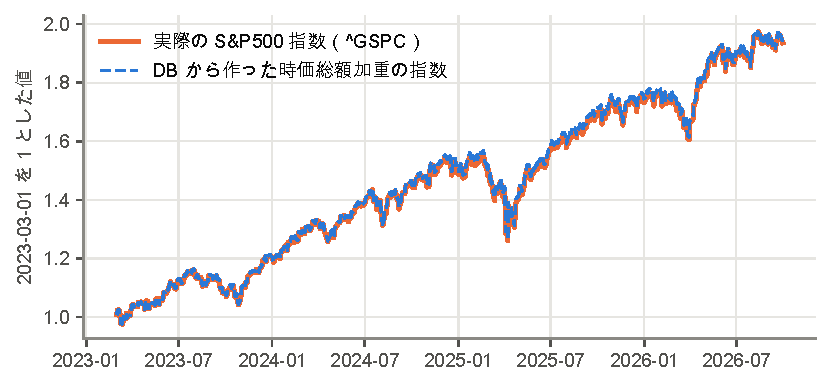
\includegraphics[width=0.92\linewidth]{index_check.pdf}
\caption{データベースから作った指数と、実際の \SP{} 指数。2 本の線はほぼ重なる。}
\label{fig:indexcheck}
\end{figure}

\begin{table}[htbp]
\centering
\caption{実際の指数との一致度。}
\small
\resizebox{\linewidth}{!}{%
\begin{tabular}{lr@{\hspace{10mm}}lrrr}
\toprule
\multicolumn{2}{l}{日次リターン} & 年 & データベース & 実際の指数 & 差 \\
\midrule
相関 & 0.9997 & 2023（3 月〜） & $+20.94\%$ & $+20.71\%$ & $+0.23\%$ \\
差の平均（絶対値） & 0.018\% & 2024 & $+23.97\%$ & $+23.31\%$ & $+0.66\%$ \\
差の最大 & 0.138\% & 2025 & $+16.38\%$ & $+16.39\%$ & $-0.01\%$ \\
差の標準偏差（年率） & 0.38\% & 2026（〜9 月） & $+11.21\%$ & $+11.77\%$ & $-0.56\%$ \\
 & & 全期間 & $+94.07\%$ & $+93.64\%$ & $+0.43\%$ \\
\bottomrule
\end{tabular}}
\end{table}

年ごとの差は最大で 0.7\% ポイント程度である。したがって、戦略と指数の差が年 1\% 未満なら、データの近似による差と区別できないと考える。

\section{実際の \SP{} と違う点}

\begin{longtable}{p{3.00cm}p{4.20cm}p{4.40cm}p{2.40cm}}
\toprule
\textbf{項目} & \textbf{実際の \SP{}} & \textbf{このデータベース} & \textbf{影響} \\
\midrule
\endfirsthead
\toprule
\textbf{項目} & \textbf{実際の \SP{}} & \textbf{このデータベース} & \textbf{影響} \\
\midrule
\endhead
\bottomrule
\endfoot
構成比率 & 浮動株で調整した時価総額 & 終値 $\times$ 発行済み株式数 & 中。創業者などの保有が多い銘柄の比率が大きく出る \\
株式数の更新 & 四半期ごとの見直しが基本 & 報告日から次の報告まで同じ値を使う & 小 \\
除外した銘柄 & すべて含む & 28 銘柄を除外 & 大。生存者バイアス \\
社名・ティッカー & 当時のもの & 2026 年 10 月時点のもの & 中。LLM に後の社名が伝わる \\
業種の分類 & 当時の分類 & 在籍中の銘柄は現在の分類 & 小 \\
株価の水準 & 当時の実際の株価 & 取得日の分割の基準に調整した値 & 小。リターンは同じ \\
配当 & 指数は配当を含まない & 銘柄のリターンは配当込み & 中。年 1.5〜1.7\% の差 \\
\end{longtable}

配当の扱いは、とくに注意が要る。戦略のリターンは配当込みで計算しているので、配当を含まない指数とそのまま比べると、戦略が年 1.5〜1.7\% ほど有利に見える。本書では、比べる相手を「データベースから作った時価総額加重の比率（配当込み）」にして、条件をそろえている。

\section{対応していないこと}

\begin{itemize}
\item 発行済み株式数には、前後の報告から 3\% 以上ずれた値が全体の 1.2\% ある。ならす処理は入れていない。
\item 配当込みの指数（トータルリターン指数）は入れていない。
\item 財務データは、2026 年 4〜6 月期の決算が 57 銘柄で欠けている。EDGAR にもう一度問い合わせたが、返ってくるデータ自体に入っていなかった（\chapref{ch:expC}）。
\item 上場直後の銘柄は、入力の日数が極端に短くなる。2024 年 9 月末の Amentum は入力が 4 日分しかなく、30 個の回答すべてが 1 日 $+3$〜$5\%$ という極端な値になった。
\end{itemize}

\chapter{データベースの設計}\label{ch:db}

データは、SQLite のファイル 1 つ（\code{data/blm.sqlite}、約 200 MB）に入れている。テーブルが 16、ビューが 7 ある。この章では全体の作りと決まりを述べる。カラムごとの定義は付録~\ref{app:tables} にある。スキーマの全文は、リポジトリの \code{marketdb/db/schema.sql} である。

\section{テーブルの一覧}

{\small
\begin{longtable}{p{4.20cm}p{6.20cm}r}
\toprule
\textbf{テーブル} & \textbf{内容} & \textbf{行数} \\
\midrule
\endfirsthead
\toprule
\textbf{テーブル} & \textbf{内容} & \textbf{行数} \\
\midrule
\endhead
\bottomrule
\endfoot
\texttt{tickers} & 銘柄・指数・セクターETFの一覧 & 584 \\
\texttt{prices} & 日次の株価 & 495,953 \\
\texttt{shares\_\allowbreak{}outstanding} & 発行済み株式数の履歴 & 175,617 \\
\texttt{index\_\allowbreak{}changes} & S\&P500 の銘柄入れ替え & 412 \\
\texttt{index\_\allowbreak{}membership} & 銘柄ごとの在籍期間 & 569 \\
\texttt{financial\_\allowbreak{}items} & 財務諸表の項目 & 6,579 \\
\texttt{financial\_\allowbreak{}facts} & 財務諸表の値 & 2,306,891 \\
\texttt{llm\_\allowbreak{}runs} & LLM の実行 & 1 \\
\texttt{llm\_\allowbreak{}views} & LLM の回答 & 440,640 \\
\texttt{portfolio\_\allowbreak{}runs} & 比率の計算 & 6 \\
\texttt{portfolio\_\allowbreak{}weights} & 比率 & 87,924 \\
\texttt{sector\_\allowbreak{}metrics} & セクターごとの指標 & 3,586 \\
\texttt{stock\_\allowbreak{}metrics} & 銘柄ごとの指標 & 256,037 \\
\texttt{reports} & 月次レポートのファイル & 39 \\
\texttt{report\_\allowbreak{}runs} & レポートの分析 & 2 \\
\texttt{report\_\allowbreak{}values} & レポートから読み取った値 & 984 \\
\end{longtable}
}

\begin{longtable}{p{4.60cm}p{9.80cm}}
\toprule
\textbf{ビュー} & \textbf{内容} \\
\midrule
\endfirsthead
\bottomrule
\endfoot
\code{market\_caps} & 取引日ごとの時価総額（終値 $\times$ その日に有効な株式数） \\
\code{index\_weights} & 日次の構成比率（在籍している銘柄の時価総額の割合） \\
\code{fundamentals\_quarterly} & 四半期ごとの主な財務項目（1 社・1 四半期で 1 行） \\
\code{llm\_view\_stats} & LLM の回答の平均と分散。Black-Litterman の $Q$ と $\Omega$ \\
\code{portfolio\_returns} & 比率を翌月末まで持ち続けた場合のリターン \\
\code{sector\_metric\_scores} & セクターの指標と、セクターの間での偏差（z スコア） \\
\code{stock\_metric\_scores} & 銘柄の指標と、同じセクターの中での順位（百分位） \\
\end{longtable}

ビューはデータを保存せず、読むたびにテーブルから計算する。共分散、均衡リターン、Black-Litterman の事後の期待リターンも保存せず、比率を計算するときに株価から作る。

\section{テーブルのつながり}

\begin{figure}[htbp]
\centering
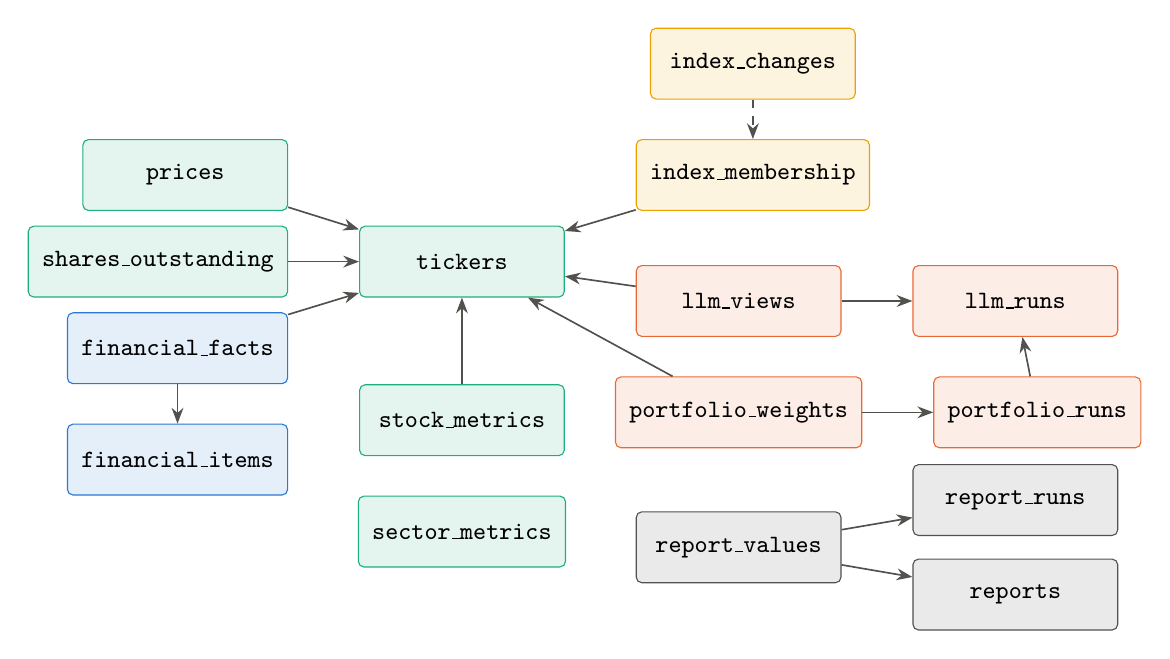
\begin{tikzpicture}[node distance=5mm and 9mm,every node/.style={font=\scriptsize}]
\node[box=c3,minimum width=26mm] (tk) {\code{tickers}};
\node[box=c3,minimum width=26mm,left=of tk,yshift=11mm] (pr) {\code{prices}};
\node[box=c3,minimum width=26mm,left=of tk] (sh) {\code{shares\_outstanding}};
\node[box=c1,minimum width=26mm,left=of tk,yshift=-11mm] (ff) {\code{financial\_facts}};
\node[box=c1,minimum width=26mm,below=of ff] (fi) {\code{financial\_items}};
\node[box=c4,minimum width=26mm,right=of tk,yshift=11mm] (im) {\code{index\_membership}};
\node[box=c4,minimum width=26mm,above=of im] (ic) {\code{index\_changes}};
\node[box=c2,minimum width=26mm,right=of tk,yshift=-5mm] (lv) {\code{llm\_views}};
\node[box=c2,minimum width=26mm,right=of lv] (lr) {\code{llm\_runs}};
\node[box=c2,minimum width=26mm,below=of lv] (pw) {\code{portfolio\_weights}};
\node[box=c2,minimum width=26mm,right=of pw] (prn) {\code{portfolio\_runs}};
\node[box=c3,minimum width=26mm,below=of tk,yshift=-6mm] (sm) {\code{stock\_metrics}};
\node[box=c3,minimum width=26mm,below=of sm] (sem) {\code{sector\_metrics}};
\node[box=ink2,minimum width=26mm,below=of pw,yshift=-3mm] (rv) {\code{report\_values}};
\node[box=ink2,minimum width=26mm,right=of rv,yshift=6mm] (rr) {\code{report\_runs}};
\node[box=ink2,minimum width=26mm,right=of rv,yshift=-6mm] (rp) {\code{reports}};
\draw[arr] (pr) -- (tk);
\draw[arr] (sh) -- (tk);
\draw[arr] (ff) -- (tk);
\draw[arr] (ff) -- (fi);
\draw[arr] (im) -- (tk);
\draw[arr,dashed] (ic) -- (im);
\draw[arr] (lv) -- (tk);
\draw[arr] (lv) -- (lr);
\draw[arr] (pw) -- (tk);
\draw[arr] (pw) -- (prn);
\draw[arr] (prn) -- (lr);
\draw[arr] (sm) -- (tk);
\draw[arr] (rv) -- (rr);
\draw[arr] (rv) -- (rp);
\end{tikzpicture}
\caption{テーブルのつながり。矢印は外部キーの向き（参照する側から、される側へ）。破線は「入れ替えの履歴から在籍期間を作る」関係で、外部キーではない。\code{sector\_metrics} のセクター名は \code{tickers} のセクター名と同じだが、外部キーは張っていない。}
\label{fig:er}
\end{figure}

\section{設計の決まり}

\begin{description}[leftmargin=2em,style=nextline,itemsep=0.4em]
\item[日付は文字列で持つ] SQLite には日付の型がない。\code{2024-07-01} の形なら、文字列の大小の比較がそのまま日付の前後の比較になる。
\item[ティッカーは yfinance の書き方] Wikipedia の \code{BRK.B} ではなく \code{BRK-B} で統一する。
\item[取得した日時を残す] Wikipedia の一覧も yfinance の値も、取得した時期で変わる。どの行にも取得日時を持たせている。
\item[外部キーは接続のたびに有効にする] SQLite は、設定を有効にしないと外部キーを確かめない。接続の関数の中で必ず有効にしている。
\item[フラグではなく期間で持つ] 「今メンバーか」のフラグでは、過去の時点の構成銘柄が答えられない。在籍の開始日と終了日で持つ。
\item[計算できるものは保存しない] 時価総額、構成比率、回答の平均と分散、翌月のリターンは、ビューで計算する。保存すると、元のデータとずれるおそれがある。
\item[実行の条件と結果を分ける] LLM の実行、レポートの読み取り、比率の計算は、「1 回の実行の条件」のテーブルと「結果」のテーブルに分ける。条件を変えたら新しい実行番号になり、古い結果は残る。
\item[変わりうる項目は縦に持つ] セクターの指標、銘柄の指標、レポートから読み取った値は、「対象・項目名・値」の 3 つ組で 1 行にする。項目を足しても、テーブルを作り直さずに済む。
\item[「株式」は在籍の記録がある銘柄] \code{tickers} には指数（\code{\textasciicircum GSPC} など）とセクター ETF も入っている。株式だけを選ぶときは、在籍期間のテーブルに行がある銘柄を選ぶ。
\end{description}

\section{制約による不正なデータの防止}

テスト用のデータベースに、わざと不正なデータを入れて確かめた。次のものは、すべてデータベースが受け付けなかった。

\begin{itemize}
\item 同じ銘柄・同じ日の株価を 2 回入れる。
\item 銘柄の一覧にない銘柄の株価や在籍期間を入れる。
\item 回答の数が 0 の実行を入れる。存在しない実行番号の回答を入れる。
\item 株式数が 0 の行を入れる。在籍の開始日が終了日以降の行を入れる。
\item 同じ発行元・同じ月のレポートを 2 回入れる。ページ数が 0 のレポートを入れる。
\item レポートから読み取った 1 つの値に、数値と文章を両方入れる。同じ項目の値を 2 回入れる。
\item 同じ判断日・セクター・指標の値を 2 回入れる。
\end{itemize}

一方で、SQLite の制約には穴もある。重複を防ぐ制約は、空の値（NULL）どうしを「別の値」とみなす。追加だけ・除外だけの入れ替えの記録は二重登録を防げないので、取得する処理の側で防いでいる。

\section{問い合わせの例}

\begin{lstlisting}[language=SQL,caption={ある判断日の Black-Litterman の入力（ビューと不確かさ）}]
SELECT symbol, n_answers, mean_return, variance
FROM llm_view_stats
WHERE run_id = 1 AND as_of_date = '2025-06-30';
\end{lstlisting}

\begin{lstlisting}[language=SQL,caption={戦略ごとの月次リターン}]
SELECT r.strategy, p.as_of_date, p.end_date, p.n_holdings, p.period_return
FROM portfolio_returns p JOIN portfolio_runs r USING (portfolio_id)
ORDER BY p.as_of_date, r.portfolio_id;
\end{lstlisting}

\begin{lstlisting}[language=SQL,caption={判断日までに公表されていた最新のレポート}]
SELECT report_id, report_month, published_date FROM reports
WHERE published_date <= '2024-03-28' ORDER BY published_date DESC LIMIT 1;
\end{lstlisting}

\chapter{LLM による予想の収集}\label{ch:views}

この章では、既存手法と同じ入力で集めた予想（実行番号 1）について、集め方と、回答の性質を述べる。

\section{集め方}

\begin{longtable}{p{3.60cm}p{10.80cm}}
\toprule
\textbf{項目} & \textbf{内容} \\
\midrule
\endfirsthead
\bottomrule
\endfoot
モデル & gpt-4o-mini（実際に答えた版は \code{gpt-4o-mini-2024-07-18}）。回答の乱数の強さ（temperature）は 1.0 \\
判断日 & 2024-03-28 から 2026-08-31 までの 30 か月の、各月の最後の取引日。予想の対象は、それぞれの翌月 \\
対象の銘柄 & 判断日に指数に在籍していて、除外していない銘柄。月あたり 482〜499 銘柄、のべ 14,688 件 \\
渡す情報 & ティッカー、社名、セクター、サブ業種、その月の日次リターン（調整後終値から計算。約 20 個） \\
渡さない情報 & 日付、株価の水準、ニュース、判断日より後のデータ \\
答えさせるもの & 翌月の平均日次リターン（小数。0.001 が 1 日 $+0.1\%$） \\
回答の数 & 1 回のリクエストで 30 個。それぞれ独立に生成される \\
\end{longtable}

プロンプトの全文は、付録~\ref{app:prompts} のリスト~\ref{lst:run1} にある。

\section{公式実装から変えた点}

\begin{longtable}{p{3.20cm}p{4.40cm}p{4.20cm}p{2.60cm}}
\toprule
\textbf{項目} & \textbf{公式実装} & \textbf{本プロジェクト} & \textbf{理由} \\
\midrule
\endfirsthead
\toprule
\textbf{項目} & \textbf{公式実装} & \textbf{本プロジェクト} & \textbf{理由} \\
\midrule
\endhead
\bottomrule
\endfoot
モデル & Llama、Gemma、Qwen & gpt-4o-mini のみ & OpenAI の API だけで再現する \\
回答の集め方 & 同じ質問を 30 回送る & 1 回送って 30 個を受け取る & 時間が約 30 分の 1 になる \\
プロンプトの単位 & 「percentage change」と書きつつ、小数を渡す & 小数であることを明記し、例を示す & 桁の違う回答が混ざると、分散が大きく狂う \\
月の最初の日 & リターンに含まない & 前月末の終値から計算して含める & 1 日分を捨てない \\
対象の銘柄 & 実行した時点の構成銘柄 & 各月末の構成銘柄 & 先読みを避ける \\
結果の保存 & 月ごとの JSON & データベース & 中断しても再開できる \\
\end{longtable}

\section{回答の確認}

\begin{longtable}{p{6.40cm}p{8.00cm}}
\toprule
\textbf{確かめたこと} & \textbf{結果} \\
\midrule
\endfirsthead
\bottomrule
\endfoot
聞くべき銘柄すべてに回答があるか & 14,688 件すべてにある \\
回答が 30 個そろっているか & そろっていない銘柄・月は 0 件 \\
読み取れなかった回答 & 0 個（440,640 個のうち） \\
桁のおかしい回答（1 日 $\pm 5\%$ 以上） & 4 個 \\
回答の範囲 & 最小 $-4.44\%$、下位 1\% が $-0.99\%$、中央値 $+0.20\%$、上位 1\% が $+1.43\%$、最大 $+7.46\%$ \\
プラスの回答の割合 & 76.2\%（平均は $+0.184\%$） \\
30 個すべてが同じ回答の銘柄・月 & 0 件 \\
\end{longtable}

単位を明記したプロンプトでは、約 44 万個の回答に、小数とパーセントの取り違えは見当たらなかった。回答の分布は \figref{fig:hist} のとおりで、プラスの側に寄っている。

\begin{figure}[htbp]
\centering
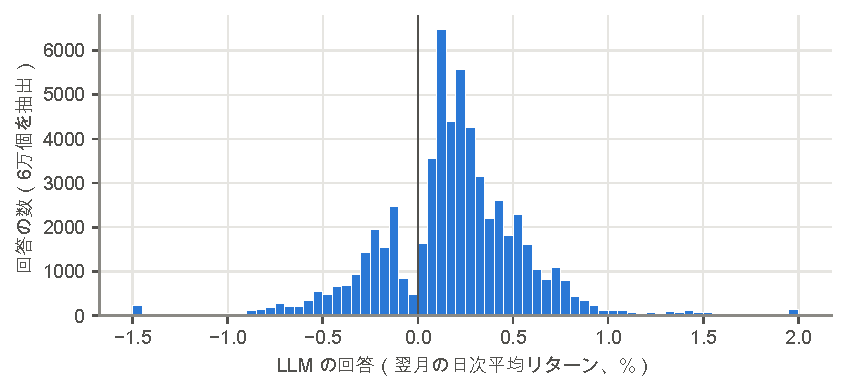
\includegraphics[width=0.88\linewidth]{answers_hist.pdf}
\caption{LLM の回答の分布（6 万個を無作為に抽出。両端は $-1.5\%$ と $+2.0\%$ にまとめた）。0 のすぐ右に山があり、プラスの回答が 76\% を占める。}
\label{fig:hist}
\end{figure}

\section{予想の性質}

\subsection{予想は入力の写しである}

各判断日について、銘柄ごとの「予想（30 個の平均）」と「渡した月の日次リターンの平均」を比べた（\figref{fig:viewinput}）。

\begin{figure}[htbp]
\centering
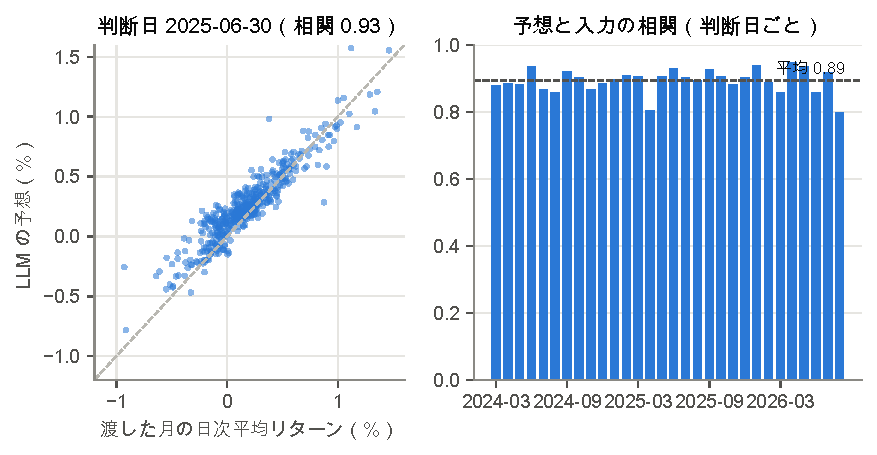
\includegraphics[width=\linewidth]{view_vs_input.pdf}
\caption{左：ある判断日の、入力の平均と予想の関係（点は銘柄）。右：判断日ごとの相関。}
\label{fig:viewinput}
\end{figure}

\begin{itemize}
\item 銘柄の間の相関は、30 か月の平均で 0.89（最小 0.80、最大 0.95）である。
\item 回帰の傾きは平均 0.77 である。渡した月の平均が 1 日 $+1\%$ なら、予想は約 $+0.77\%$ になる。
\item 回答のばらつき（30 個の標準偏差）は、渡した月の値動きの大きさと順位相関が 0.73 ある。値動きの大きい銘柄ほど、回答がばらつく。
\end{itemize}

つまり、「LLM に聞く」ことと「先月の平均リターンを計算する」ことが、ほぼ同じ情報になっている。

\subsection{予想は楽観的で、ほとんど当たっていない}

\begin{itemize}
\item 全銘柄・全月の予想の平均は、1 日 $+0.18\%$（1 か月で約 $+4\%$）である。同じ銘柄の翌月の実際のリターンは、1 日あたり $+0.04\%$ だった。予想は、実際の約 4 倍の上昇を見込んでいる\footnote{以前の資料とスライドでは、実際の値を「$+0.02\%$」、倍率を「約 8 倍」と書いていた。本書を作るときに、翌月の騰落率を取引日数で割る形で計算し直したところ、$+0.044\%$ だった。等金額の戦略の年率リターン（$+10.1\%$）とも合うので、本書ではこの値を使う。}。
\item 予想と翌月の実際のリターンの順位相関は、30 か月の平均で $+0.05$ である。プラスの月は 30 か月のうち 14 か月で、月によって $-0.33$ から $+0.35$ まで振れる（\figref{fig:rankic}）。
\end{itemize}

\begin{figure}[htbp]
\centering
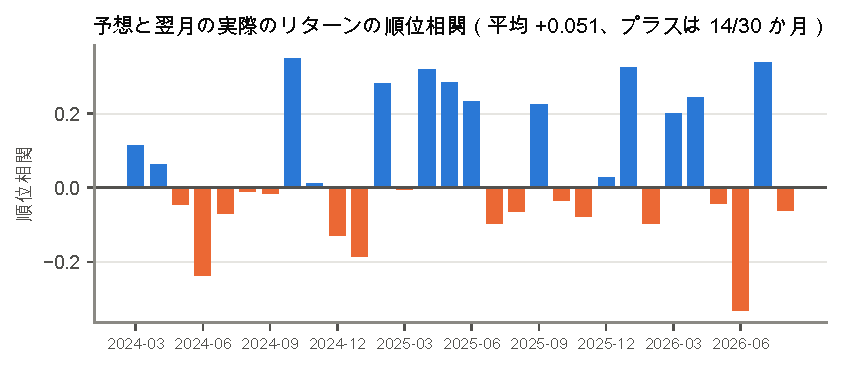
\includegraphics[width=0.92\linewidth]{rank_ic.pdf}
\caption{予想と翌月の実際のリターンの順位相関（判断日ごと）。}
\label{fig:rankic}
\end{figure}

入力が 1 か月分の日次リターンだけなので、当たらないこと自体は不自然ではない。問題は、この当たらない予想が、次の章で見るように、Black-Litterman の中で強く信じられてしまうことである。月ごとの数値は、付録~\ref{app:monthly} の表にある。

\section{使うときの注意}

\begin{description}[leftmargin=2em,style=nextline,itemsep=0.4em]
\item[モデルの知識の期限] gpt-4o-mini の学習データは、2023 年 10 月までとされている。入力は 2024 年 3 月以降なので、モデルが答えを知っている期間とは重ならない。新しいモデルに替えると、評価期間の値動きを知っている可能性が出る。
\item[実行のたびに回答が変わる] 分析では、必ず実行番号を指定する。
\item[社名から後の情報が伝わる] 社名とティッカーは 2026 年 10 月時点のものである。プロンプトに日付は入れていないが、後の社名の変更は伝わる。
\end{description}

\chapter{比率の計算と最初の結果}\label{ch:blm}

この章では、LLM の予想から比率を計算する部分（\code{blm/}）と、6 つの戦略を 30 か月分比べた結果を述べる。

\section{計算した戦略}

\begin{longtable}{p{3.60cm}p{3.60cm}p{3.20cm}p{4.00cm}}
\toprule
\textbf{戦略} & \textbf{期待リターン} & \textbf{共分散} & \textbf{比率の決め方} \\
\midrule
\endfirsthead
\toprule
\textbf{戦略} & \textbf{期待リターン} & \textbf{共分散} & \textbf{比率の決め方} \\
\midrule
\endhead
\bottomrule
\endfoot
時価総額加重 & --- & --- & 判断日の時価総額の比率そのまま \\
等金額 & --- & --- & 全銘柄に同じ比率 \\
平均分散（元の計算） & 判断月の日次リターンの平均 & 判断月の約 20 日分 & 公式実装の最適化（SciPy の標準の設定） \\
BL（元の計算） & 公式実装の式（\secref{sec:original-calc}） & 判断月の約 20 日分 & 公式実装の最適化 \\
平均分散（直した計算） & 過去 1 年の日次リターンの平均 & 過去 1 年、縮小推定 & 二次計画の解法で最後まで解く \\
BL（直した計算） & 逆最適化の均衡リターンを、LLM の予想で修正 & 過去 1 年、縮小推定 & 二次計画の解法で最後まで解く \\
\end{longtable}

「元の計算」は、公式実装の式、係数（$\tau = 0.025$、リターンの重み 0.1、金利 0.02）、最適化の方法と設定を、そのまま写したものである。「直した計算」は、\chapref{ch:theory} の標準の形にしたものである。違いは 3 つある。

\begin{enumerate}
\item \textbf{事前の期待リターン}：元はベータから作り、年率の金利を日次のリターンから引く。直した計算は、時価総額の比率から逆算する（式~\eqref{eq:implied}）。
\item \textbf{共分散}：元は判断月の約 20 日分の標本共分散。直した計算は、過去 252 取引日に Ledoit-Wolf の縮小推定を使う。
\item \textbf{最適化}：元は SciPy の汎用の解法（SLSQP）を標準の設定で使う。直した計算は、二次計画用の解法（CVXPY と Clarabel）で最適解まで解く。
\end{enumerate}

戦略の定義は、リスト~\ref{lst:strategies} のとおりである。

\begin{lstlisting}[language=Python,caption={戦略の定義（\code{blm/strategies.py} の主要部）},label={lst:strategies}]
def black_litterman(inputs):
    """Market equilibrium corrected by the LLM views."""
    covariance = shrunk_covariance(inputs.returns)
    prior = implied_returns(covariance, inputs.market_weights, config.RISK_AVERSION)
    views = inputs.view_mean - inputs.risk_free_daily
    expected = posterior_returns(prior, covariance, views, inputs.view_variance, config.TAU)
    return optimize(expected, covariance, config.RISK_AVERSION)

def black_litterman_original(inputs):
    """The calculation of the original implementation, on the same universe and views."""
    covariance = sample_covariance(inputs.month_returns)
    prior = capm_returns_original(inputs.month_returns, inputs.market_weights,
                                  config.ORIGINAL_RISK_FREE_RATE)
    expected = posterior_returns_original(prior, covariance, inputs.view_mean,
                                          inputs.view_variance, config.TAU)
    return optimize_original(expected, covariance, config.ORIGINAL_RETURN_WEIGHT)
\end{lstlisting}

\section{計算の条件}

\begin{description}[leftmargin=2em,style=nextline,itemsep=0.3em]
\item[対象の銘柄] 判断日に指数に在籍し、LLM の予想と時価総額があり、過去 1 年のうち半分以上の日に株価がある銘柄。全戦略で同じ銘柄を使う（平均 488 銘柄）。
\item[リターンの計算] 判断日の終値で買い、翌月の最後の取引日まで持ち続ける。配当込みで、売買のコストは入れていない。
\item[無リスク金利] 3 か月物の米国債の利回りを、日次に直して使う。
\item[係数] $\tau = 0.025$、リスク回避度 $\delta = 2.5$。使った値は、比率と一緒にデータベースに保存している。
\end{description}

計算の仕組みが正しいことは、2 つの方法で確かめた。

\begin{itemize}
\item \textbf{均衡の確認}：予想を入れずに、均衡リターンをそのまま最適化に入れると、結果は時価総額の比率に一致した（ずれは 0.001\% 未満）。
\item \textbf{指数との照合}：時価総額加重の戦略の成績は、実際の \SP{} 指数とほぼ同じ動きをした。年率の差（$+1.5\%$）は、配当を含むかどうかの違いである。
\end{itemize}

\section{成績}

\begin{table}[htbp]
\centering
\caption{30 か月（判断日 2024-03-28〜2026-08-31）の成績。「対 時価総額」は、時価総額加重との月次リターンの差を年率にしたもの。}
\label{tab:perf}
{\footnotesize
\resizebox{\linewidth}{!}{%
\begin{tabular}{lrrrrrrr}
\toprule
戦略 & 年率リターン & 年率リスク & シャープ & 最大下落率 & 最悪の月 & 対 時価総額 & 上回った月 \\
\midrule
時価総額加重 & +17.7\% & 12.2\% & 1.06 & -7.7\% & -5.8\% & --- & --- \\
等金額 & +10.1\% & 11.7\% & 0.52 & -8.9\% & -6.3\% & -6.8\% & 14/30 \\
平均分散（元の計算） & +29.4\% & 24.8\% & 0.99 & -14.0\% & -12.7\% & +11.7\% & 16/30 \\
BL（元の計算） & +35.0\% & 23.5\% & 1.22 & -10.2\% & -10.2\% & +15.8\% & 16/30 \\
平均分散（直した計算） & +149.0\% & 93.7\% & 1.34 & -46.6\% & -46.6\% & +112.2\% & 19/30 \\
BL（直した計算） & +11.0\% & 51.4\% & 0.40 & -45.0\% & -45.0\% & +7.6\% & 16/30 \\
参考：S\&P500 指数（配当なし） & +16.2\% & 12.1\% & 0.96 & -7.8\% & -5.8\% & -1.3\% & 6/30 \\
\bottomrule
\end{tabular}}
}
\end{table}

\begin{figure}[htbp]
\centering
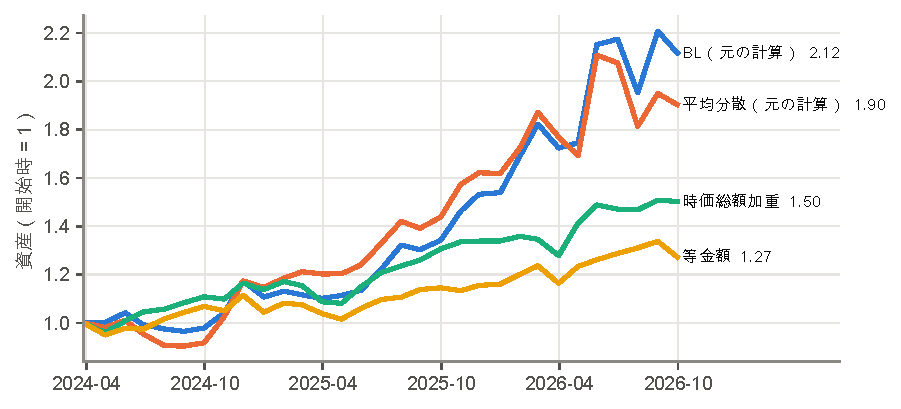
\includegraphics[width=0.95\linewidth]{cumret_original.pdf}
\caption{元の計算による戦略と、時価総額加重、等金額の資産の推移。}
\label{fig:cumorig}
\end{figure}

\begin{figure}[htbp]
\centering
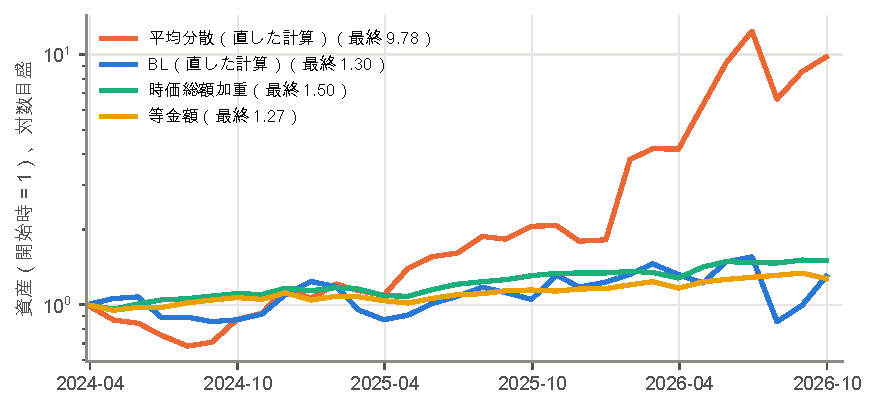
\includegraphics[width=0.95\linewidth]{cumret_fixed.pdf}
\caption{直した計算による戦略の資産の推移（縦軸は対数目盛）。平均分散は、1 銘柄にほぼ全額を入れた結果である。}
\label{fig:cumfixed}
\end{figure}

数字だけを見ると、元の計算の Black-Litterman が年率 $+35.0\%$ で最も良く見える。しかし、この数字から「LLM と Black-Litterman が効いた」と読むことはできない。理由は 2 つある。

第 1 に、月ごとの差のばらつきが大きく、偶然と区別できない。元の計算の Black-Litterman と時価総額加重の差は、年率で $+15.8\%$ だが、月ごとの差の標準偏差は 6.2\% あり、$t$ 値は 1.16 である（目安は 2 以上）。リスクは時価総額加重の約 2 倍ある。

第 2 に、最適化した戦略はどれも、少数の銘柄への賭けになっている。次の節で示す。

\section{比率の集中}

\begin{table}[htbp]
\centering
\caption{比率の集中と入れ替わり（30 か月の平均）。}
\label{tab:conc}
{\small
\begin{tabular}{lrrr}
\toprule
戦略 & 実質的な銘柄数 & 最大の比率（平均） & 毎月入れ替わる割合 \\
\midrule
時価総額加重 & 51.5 & 7\% & 3\% \\
等金額 & 488.5 & 0\% & 0\% \\
平均分散（元の計算） & 9.4 & 22\% & 96\% \\
BL（元の計算） & 9.9 & 19\% & 96\% \\
平均分散（直した計算） & 1.5 & 79\% & 24\% \\
BL（直した計算） & 1.7 & 78\% & 100\% \\
\bottomrule
\end{tabular}
}
\end{table}

\begin{figure}[htbp]
\centering
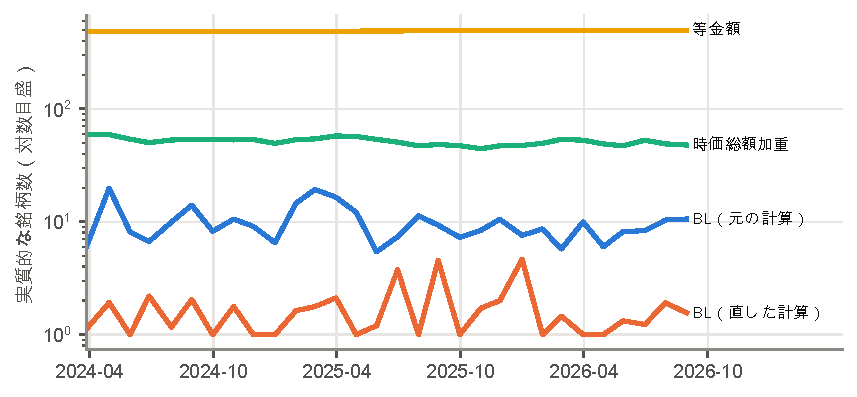
\includegraphics[width=0.92\linewidth]{effective_holdings.pdf}
\caption{実質的な銘柄数の推移（縦軸は対数目盛）。}
\label{fig:effhold}
\end{figure}

直した計算の Black-Litterman は、実質 1.7 銘柄しか持っていない。最大の比率は平均で 78\% で、毎月ほぼ全部が入れ替わる。「市場の比率を、LLM の予想で少し調整する」という、Black-Litterman 本来の形になっていない。

平均分散（直した計算）も同じで、過去 1 年で最も上がった銘柄に集中する。最大の比率になった銘柄は、Palantir が 9 か月、SanDisk が 9 か月、Vistra が 7 か月だった。年率 $+149\%$ という数字は、たまたま選ばれた数銘柄の値動きを映しているだけである。

\section{なぜ集中するか}

成績を見ずに、比率の形だけで原因を調べた。

\begin{longtable}{p{8.20cm}p{6.20cm}}
\toprule
\textbf{比べるもの} & \textbf{大きさ} \\
\midrule
\endfirsthead
\bottomrule
\endfoot
市場の均衡が示すリターン（全銘柄の平均） & 1 日 $+0.01$〜$0.03\%$ \\
LLM の予想（全銘柄の平均） & 1 日 $-0.17$〜$+0.28\%$（月による）。均衡の約 10 倍 \\
LLM の回答の分散 $\div$（$\tau \times$ 銘柄の分散） & 中央値で 0.10〜0.29。予想のほうが、均衡より数倍信頼されている \\
LLM の回答の分散 $\div$ 実際の予測誤差の目安 & 中央値で 0.05〜0.15。実際の 10〜20 倍の自信を持っていることになる \\
\end{longtable}

「実際の予測誤差の目安」は、銘柄の日次リターンの分散を 21 日で割った値で、1 か月の平均リターンがどれだけぶれるかを表す。

原因は、LLM の予想が大きすぎることと、それが強く信じられることである。銘柄どうしの予想の差が、リスクに比べて大きすぎるので、「予想が最も高い銘柄に全部入れる」が最適になる。設定を少し変えても、この形は変わらなかった（\tabref{tab:tryset}）。

\begin{table}[htbp]
\centering
\caption{設定を変えたときの比率の形（10 か月分。成績は見ていない）。}
\label{tab:tryset}
\small
\begin{tabular}{p{7.00cm}rrr}
\toprule
変えたこと & 実質的な銘柄数 & 最大の比率 & 指数からのずれ（年率） \\
\midrule
今回の設定（リスク回避度 2.5） & 1.9 & 76\% & 37\% \\
リスク回避度を 20 にする & 5.0 & 32\% & 19\% \\
予想を「全銘柄の平均との差」に直す & 1.9 & 72\% & 37\% \\
予想の不確かさを、実際の予測誤差の目安に置き換える & 1.8 & 75\% & 36\% \\
上の 2 つを両方行う & 1.9 & 70\% & 36\% \\
\bottomrule
\end{tabular}
\end{table}

\section{元の計算が分散して見える理由}

元の計算の Black-Litterman は、実質 9.9 銘柄に分かれている。直した計算より「まとも」に見えるが、これは計算の不備が重なった結果である。最適化が途中で止まり、出発点（全銘柄に同じ比率）の名残で、多くの銘柄に分かれている。同じ目的関数を最後まで解くと、実質 4.2 銘柄になる。くわしくは次の章で述べる。

直した計算で 1〜2 銘柄に集中するのは、計算を正しくしたことで、「予想が大きすぎる」という元からあった問題が、そのまま表に出たためである。

\section{次に決めること}

「市場の比率を、LLM の予想で少し調整する」形にするには、予想の大きさか、指数からのずれのどちらかを抑える必要がある。

\begin{longtable}{p{3.80cm}p{5.40cm}p{5.20cm}}
\toprule
\textbf{案} & \textbf{内容} & \textbf{評価} \\
\midrule
\endfirsthead
\bottomrule
\endfoot
A. 指数からのずれに上限を付ける & 最適化に「時価総額加重とのずれ（年率）を $X\%$ 以内」という条件を足す & 目的にそのまま合う。実務でも普通のやり方。$X$ は成績を見ずに決める \\
B. 予想を当たり具合に合わせて縮める & $\Omega$ を回答のばらつきではなく、予想が実際にどれだけ当たるかから決める。式~\eqref{eq:grinold} もこの考え方 & Black-Litterman の考え方として筋が通る。当たり具合を測る期間と、使う期間を分ける必要がある \\
C. 1 銘柄の比率に上限を付ける & たとえば「時価総額の比率の $\pm 1\%$ まで」 & 単純だが根拠が弱い。上限に張り付いた比率になりやすい \\
\end{longtable}

どれを採るかは、まだ決めていない。この章の成績は、設定を選ぶための材料にはしない。評価期間の成績を見て設定を選ぶと、それ自体が先読みになるためである。

% ============================================================
\part{元論文の計算の検証}
% ============================================================

\chapter{元論文の計算の問題点}\label{ch:problems}

この章では、公式実装の計算をそのまま再現し、30 か月分のデータで確かめた問題点をまとめる。

\begin{keybox}
元の計算は、名前は「LLM の予想と Black-Litterman」だが、実際には「先月よく上がった銘柄を十数個選ぶ」計算に近い。成績は良く見えるが、LLM と Black-Litterman の効果だとは言えない。
\begin{itemize}
\item Black-Litterman が、均衡から LLM の予想へ動かす割合は、中央値で 99.9\% である。
\item LLM の予想と、渡した月の平均リターンの相関は 0.89 である。
\item 元の最適化の結果は実質 9.9 銘柄だが、同じ式を最後まで解くと 4.2 銘柄になる。
\item 計算に使われている「市場の均衡リターン」の平均は、1 日あたり $-1.4\%$ という、あり得ない値である。
\end{itemize}
\end{keybox}

\section{確かめた範囲}

\begin{longtable}{p{3.40cm}p{11.00cm}}
\toprule
\textbf{項目} & \textbf{内容} \\
\midrule
\endfirsthead
\bottomrule
\endfoot
再現した計算 & Black-Litterman（\code{evaluate\_multiple.py}）と、比べる相手の平均分散（\code{baselines.py}）。式、係数、最適化の方法と設定は公式実装と同じ \\
使ったデータ & 判断日 2024-03-28〜2026-08-31 の 30 か月、月あたり 479〜497 銘柄。LLM は gpt-4o-mini（約 44 万個の回答） \\
数字の出どころ & とくに断りがなければ、30 か月すべてで計算した値 \\
\end{longtable}

\begin{notebox}
ここで確かめたのは「公式実装の計算」であり、論文の数字そのものではない。モデル（論文は Llama、Gemma、Qwen）と期間が違う。構成銘柄、時価総額、プロンプトの単位は、こちらで直したものを使っている。論文のモデルで同じことが起きているかは、論文のデータで確かめる必要がある。
\end{notebox}

\section{問題点の一覧}

\begin{longtable}{rp{4.40cm}p{6.20cm}p{1.60cm}p{1.60cm}}
\toprule
 & \textbf{問題} & \textbf{一言で} & \textbf{影響} & \textbf{確かめ方} \\
\midrule
\endfirsthead
\toprule
 & \textbf{問題} & \textbf{一言で} & \textbf{影響} & \textbf{確かめ方} \\
\midrule
\endhead
\bottomrule
\endfoot
1 & Black-Litterman が働いていない & 均衡と予想を「混ぜる」はずが、予想を 99.9\% 採用している & 大 & 計算 \\
2 & 予想が先月の値動きの写し & 予想は、渡した月の平均リターンにほぼ比例する & 大 & 計算 \\
3 & ばらつきは信頼度ではない & 回答がそろっていても、当たるとは限らない & 大 & 計算 \\
4 & 最適化が途中で止まる & 報告される比率は、式の最適な答えではない & 大 & 計算 \\
5 & 均衡リターンの単位 & 日次のリターンから、年率の金利を引いている & 小 & 計算 \\
6 & 共分散のデータ不足 & 約 490 銘柄の連動を、約 20 日分で計算している & 中 & 計算 \\
7 & 先読みと銘柄の選び方 & 構成銘柄と時価総額が、後の時点のもので固定 & 中 & コード \\
8 & リターンの計算と売買のコスト & 毎月ほぼ全部を入れ替えるのに、コストがゼロ & 中 & 計算 \\
9 & 細かい取りこぼし & 単位の食い違い、月末日の欠落など & 小 & コード \\
\end{longtable}

\section{問題 1：Black-Litterman が働いていない}

Black-Litterman は、市場の均衡リターンと予想を、自信の度合いに応じて混ぜる方法である。ところが元の計算では、混ぜた後の期待リターンが、LLM の予想とほとんど同じになっている。

\begin{longtable}{p{8.40cm}p{6.00cm}}
\toprule
\textbf{確かめたこと} & \textbf{結果（30 か月）} \\
\midrule
\endfirsthead
\bottomrule
\endfoot
混ぜた後の値は、均衡から予想へ何 \% 動いたか & 中央値で 99.87\%（最小 99.75\%） \\
混ぜた後の値と、LLM の予想の相関 & 中央値 0.997 \\
均衡リターンをすべて 0 に変えたら、比率は変わるか & ほとんど変わらない。元の比率と平均 92\% が重なる \\
Black-Litterman を使わず、予想をそのまま最適化に入れたら & ほぼ同じ比率になる。平均 89\% が重なる \\
\end{longtable}

「比率の重なり」は、2 つの比率が共通して持っている部分の合計である（100\% なら同じ比率）。式の違いだけを見るため、どれも同じ目的関数を最後まで解いて比べている。

原因は、予想の不確かさ $\Omega$ に、30 個の回答の分散を使っていることである。この分散は小さく、式~\eqref{eq:scalar} の採用率がほぼ 1 になる。共分散を過去 1 年分・縮小推定のものに替えても、採用率は中央値で 98\%（96〜99\%）だった。約 20 日分で作った共分散（問題 6）は、これを 99.9\% まで強めている。データが足りない方向では、均衡の情報がないものとして扱われるためである。

この計算は、実質的には「LLM の予想を期待リターンにした平均分散最適化」である。できた比率は、時価総額の比率と平均 3.6\% しか重ならない。

\section{問題 2：予想が先月の値動きの写し}

\chapref{ch:views} で見たとおり、LLM の予想は、渡した月の平均リターンにほぼ比例する。その結果、Black-Litterman の比率は、比べる相手の平均分散（先月の平均リターンで最適化するもの）と似たものになる。

\begin{longtable}{p{8.40cm}p{6.00cm}}
\toprule
\textbf{確かめたこと} & \textbf{結果（30 か月）} \\
\midrule
\endfirsthead
\bottomrule
\endfoot
予想と、渡した月の平均リターンの相関 & 平均 0.89（最小 0.80、最大 0.95） \\
BL の比率と、平均分散の比率の重なり & 平均 61\% \\
BL と平均分散の、月次リターンの相関 & 0.94 \\
BL と平均分散の、月次リターンの差 & 平均 $+0.34\%$／月、標準偏差 2.43\%。$t$ 値は 0.76 で、差があるとは言えない \\
\end{longtable}

LLM が足している情報は、成績からは確認できない。

\section{問題 3：回答のばらつきは信頼度ではない}

対象論文は、30 個の回答がそろっていれば「自信がある」、ばらばらなら「自信がない」とみなす。しかし、ばらつきが示すのは「同じ質問への答えのぶれ」で、「予想が当たる度合い」ではない。

\begin{longtable}{p{8.40cm}p{6.00cm}}
\toprule
\textbf{確かめたこと} & \textbf{結果} \\
\midrule
\endfirsthead
\bottomrule
\endfoot
予想と、翌月の実際のリターンの順位相関 & 30 か月の平均で $+0.05$。プラスの月は 14 か月 \\
回答の分散 $\div$ 実際の予測誤差の目安 & 中央値で 0.05〜0.15。実際の 10〜20 倍の自信を持っていることになる \\
回答のばらつきが何で決まっているか & 渡した月の値動きの大きさ（順位相関 0.73） \\
\end{longtable}

ほとんど当たらない予想を、非常に強く信じる設定になっている。問題 1 で予想が 99.9\% 採用されるのは、このためである。ばらつきは temperature を変えれば変わるので、モデルの設定しだいで「自信」が変わってしまう、という問題もある。

\section{問題 4：最適化が途中で止まる}

比率を決める最適化（SciPy の標準の設定）が、まだ良くできる余地を残して止まっている。公式実装の最適化の結果と、同じ目的関数を二次計画用の解法で最後まで解いた結果を、30 か月すべてで比べた。

\begin{table}[htbp]
\centering
\caption{元の最適化の結果と、同じ目的関数を最後まで解いた結果。}
\small
\begin{tabular}{lrr}
\toprule
 & 元の最適化 & 最後まで解いた結果 \\
\midrule
実質的な銘柄数（平均） & 9.9 & 4.2 \\
実質的な銘柄数（最小〜最大） & 5.4〜19.8 & 2.6〜6.6 \\
比率が 0.1\% を超える銘柄数（平均） & 16.5 & 6.4 \\
\bottomrule
\end{tabular}
\end{table}

2 つの比率の重なりは平均 62\%（最小 37\%）で、残りは別の銘柄を持っている。目的関数の値で見ると、元の最適化は改善できる幅の 95\% まで進んで止まっている。残りの数 \% の間に、比率は「十数銘柄」から「4 銘柄前後」へ大きく変わる。比べる相手の平均分散でも同じで、元の最適化は実質 9.4 銘柄、最後まで解くと 4.5 銘柄である。

元の計算の比率が十数銘柄に分かれているのは、最適化が途中で止まったためである。出発点が「全銘柄に同じ比率」なので、途中で止まると、その名残で多くの銘柄に分かれる。結果は、解法の種類、止める基準、出発点に左右される。これらは論文の方法の一部として書かれていないので、同じ式を別の方法で解いた人は、違う結果を得る。

\section{問題 5：均衡リターンの単位}

市場の均衡リターンを計算するとき、日次のリターンから、年率の無リスク金利（0.02）をそのまま引いている。

\begin{lstlisting}[language=Python,caption={公式実装の該当箇所（\code{evaluate\_multiple.py}）}]
risk_free_rate = 0.02
market_risk_premium = (market_return_weighted - risk_free_rate).mean()
market_equilibrium_return = market_beta * market_risk_premium
\end{lstlisting}

30 か月の範囲で、市場のリスクプレミアムは 1 日あたり $-2.25\%$〜$-1.45\%$、均衡リターンの銘柄平均は $-1.94\%$〜$-0.57\%$ になった。「市場全体が、毎日 1〜2\% ずつ下がる」という出発点である。日次に直すなら、$0.02/252$ を引く必要がある。

これは誤りだが、結果にはほとんど影響しない。問題 1 のとおり、均衡リターンは 0.1\% しか使われていないからである。裏を返すと、「均衡が何であっても結果が変わらない」こと自体が、Black-Litterman が働いていない証拠である。

\section{問題 6：共分散のデータ不足}

約 488 銘柄の共分散を、判断月の 19〜23 日分の日次リターンだけで計算している。共分散行列の階数は 18〜22 で、逆行列は存在しない。コードは疑似逆行列で代用している。

銘柄の数よりデータの数が少ないと、共分散は正しく推定できない。ただし、この計算での影響は中くらいにとどまる。目的関数の中でリターンの項が支配的で、リスクの項は比率をあまり左右していないためである。計算上のリスク（年率 19\%）は、翌月以降の実績（年率 23\%）より小さく出る。影響が大きく出るのは、予想の大きさを現実的な水準に直した場合である。そのときは、リスクの項が比率を決めるようになる。

\section{問題 7：先読みと銘柄の選び方}

コードを読んで確かめた点である。

\begin{longtable}{p{2.60cm}p{5.20cm}p{6.60cm}}
\toprule
\textbf{箇所} & \textbf{公式実装} & \textbf{問題} \\
\midrule
\endfirsthead
\bottomrule
\endfoot
構成銘柄 & 実行した時点の Wikipedia の一覧を、全期間に使う & 後から指数に入った銘柄を、過去にさかのぼって持つ。指数に採用されるのは株価が上がった会社が多いので、成績が良く見える方向に働く \\
時価総額 & 1 つの時点の値を、全期間に使う & 過去の判断に、後の時点の時価総額を使う \\
対象の絞り込み & 全モデルで回答が得られた銘柄だけ。さらに 2 銘柄をコードの中で直接除外 & 絞り込みの基準が、結果を見た後で決まっている。除外の理由が書かれていない \\
\end{longtable}

本プロジェクトの再現では、構成銘柄と時価総額は各判断日のものを使っている。この問題の影響の大きさは、まだ測っていない。

\section{問題 8：リターンの計算と売買のコスト}

元の計算の Black-Litterman は、毎月 96\% を入れ替える。売りと買いを合わせると、毎月、資産の約 1.9 倍の売買である。片道 0.1\% のコストを仮定すると、年率で約 2.3\% の負担になる。公式実装のリターンの計算は、翌月の日次リターンに月初の比率を毎日掛けるもので、毎日比率を元に戻す（毎日売買する）計算になっている。その分のコストも入っていない。

\section{問題 9：細かい取りこぼし}

\begin{itemize}
\item プロンプトは「percentage change」と書きながら、小数を渡している。
\item 株価の取得で、毎月、最後の 1 日が抜ける。月の最初の日のリターンもない。
\item Wikipedia のティッカーの書き方のままでは、Berkshire Hathaway などの株価が取れない。
\item 読み取れない回答は黙って飛ばされ、30 個のうち何個で計算したかが残らない。
\end{itemize}

\section{元論文の結果をどう読むか}

4 つの問題をつなげると、元の計算で起きていることが説明できる。

\begin{enumerate}
\item LLM に渡した月の値動きが、そのまま予想になる（問題 2）。
\item Black-Litterman は、その予想をほぼそのまま通す（問題 1、3）。均衡リターンは、誤っていても関係がない（問題 5）。
\item 最適化が、予想の高い銘柄に集中させる。式を最後まで解けば 4 銘柄前後で、途中で止まるので十数銘柄に見える（問題 4）。
\item 結果は「先月よく上がった銘柄を、十数個持つ」比率になる。
\end{enumerate}

元の計算の成績は、「LLM の予想を Black-Litterman で市場の比率に反映した効果」とは読めない。読めるのは、「直近 1 か月の値動きが大きかった銘柄に集中した場合の成績」である。LLM と Black-Litterman のどちらを外しても、ほぼ同じ比率になる。

第 2 版の論文は「LLM ごとに一貫した投資スタイルがあり、それが成績を決める」と述べている。この見方は、上の流れと矛盾しない。モデルごとに回答のばらつきや楽観の度合いが違えば、最適化が止まる位置や、選ばれる銘柄の数が変わるからである。ただし、これは論文のデータで確かめたものではない。

\section{問題ではなかった点}

\begin{itemize}
\item \textbf{Black-Litterman の式そのもの}：コードの式は、標準の式と数学的に同じである（疑似逆行列を使っている点を除く）。問題は式ではなく、入れている値（$\Omega$ と共分散）にある。
\item \textbf{「最適化が等金額から動かない」}：5 銘柄の小さなテストではそうなったが、全銘柄では動いていた。正確には「最適な答えに届く前に止まる」である。
\item \textbf{30 回聞くこと}：1 回のリクエストで 30 個の回答を受け取っても、回答は独立に生成される。
\end{itemize}

% ============================================================
\part{拡張の設計}
% ============================================================

\chapter{設計の方針}\label{ch:policy}

再現と検証の結果を受けて、手法を拡張する計画を立てた。この章では、その方針をまとめる。実装した部分は、次の章から述べる。

\section{論点の置き方}

主役は「設計」に置く。当時知り得た情報だけで動く仕組みを作り、その上で LLM の予想を入れた比率を、時価総額加重と比べる。「どのモデルが良いか」の比較は、脇役にとどめる。対象論文がすでに行っていて、予算、期間、モデルの知識の期限の問題で、はっきりした結論を出しにくいためである。

元の論文にない要素として、示せるものを挙げる。

\begin{longtable}{p{4.60cm}p{7.40cm}p{2.40cm}}
\toprule
\textbf{要素} & \textbf{内容} & \textbf{状態} \\
\midrule
\endfirsthead
\toprule
\textbf{要素} & \textbf{内容} & \textbf{状態} \\
\midrule
\endhead
\bottomrule
\endfoot
その時点の構成銘柄 & 各判断日に在籍していた銘柄だけを対象にする & 済み \\
提出日つきの財務データ & 判断日までに公表された値だけを使える & 済み \\
実行ごとに再現できる保存 & モデルの版、プロンプト、設定、全回答を実行番号ごとに残す & 済み \\
単位を明示したプロンプト & 小数であることを明記し、桁の違う回答を防ぐ & 済み \\
安定した共分散 & 直近 1 年の日次リターンと縮小推定 & 済み \\
入力の拡張 & 値動きの要約、財務、セクター、市場、レポートの文章 & データは済み \\
統計モデルとの比較 & 同じ変数を渡した回帰と比べ、LLM が何を足しているかを示す & 未着手 \\
結果へのフィードバック & 数字で要因を分解し、当時の資料と合わせて LLM に説明させる & 未着手 \\
\end{longtable}

\section{未来の情報が混ざる経路}\label{sec:leak}

過去のデータで戦略を試すとき、判断した時点では知り得なかった情報が混ざると、成績が実力より良く見える。この研究では、混ざる経路を 1 つずつ挙げて、ふさいだかどうかを示す。

\begin{longtable}{p{2.80cm}p{4.60cm}p{5.00cm}p{2.00cm}}
\toprule
\textbf{経路} & \textbf{どう混ざるか} & \textbf{ふさぎ方} & \textbf{状態} \\
\midrule
\endfirsthead
\toprule
\textbf{経路} & \textbf{どう混ざるか} & \textbf{ふさぎ方} & \textbf{状態} \\
\midrule
\endhead
\bottomrule
\endfoot
1. モデルの知識 & LLM が、評価期間の相場を学習で知っている & 知識の期限（2023 年 10 月）が評価期間（2024 年 4 月〜）より前のモデルを使う & 済み \\
2. 渡す資料 & レポートや要約に、後から書かれた内容が混ざる & 公表日が判断日以前の資料だけを使う。AI に検索させず、渡した資料だけを整理させる & 済み（レポートの公表日を記録） \\
3. 構成銘柄 & 後から指数に入った銘柄を、過去にさかのぼって使う & 判断日に在籍していた銘柄だけを対象にする & 済み \\
4. 財務データの提出日 & まだ公表されていない決算や、後から修正された数字を使う & 提出日が判断日以前の値だけを使う。最初に提出された値を保存する & 済み \\
5. 株価と共分散 & 判断日より後の株価を、入力や共分散に使う & 判断日までのデータだけを使う & 済み \\
6. 設定の選び方 & 評価期間の成績を見て、設定やモデルを選ぶ & 選ぶ期間と、成績を示す期間を分ける & 未決定 \\
\end{longtable}

ふさぎきれていない経路もある。

\begin{itemize}
\item \textbf{除外した 28 銘柄}：「後で上場廃止になった」という情報で対象から外している。無料のデータでは株価が取れない。
\item \textbf{社名、ティッカー、セクター}：2026 年 10 月時点のものを LLM に渡している。
\item \textbf{要約に使う AI の知識}：資料の要約を新しいモデルにさせると、要約に未来の知識が混ざる可能性がある。レポートの読み取りにも gpt-4o-mini を使っているのは、このためである。
\end{itemize}

\subsection{AI に書かせたレポートで見つかった問題}

運用会社のレポートの代わりに、AI に検索させて月ごとのレポートを書かせる案を試した。試作（2025 年 1 月の日本株のセクターレポート）を調べると、対象月より後の情報が入っていた。

\begin{itemize}
\item 「自動車関税は 15\% で妥結する見通し」とあるが、日米が 15\% で合意したのは 2025 年 7 月である。
\item 引用元に、2025 年末や 2026 年 1 月に書かれた記事が含まれていた。
\item その結果、「自動車：やや強気」のような点数が、半年後の結果を知ったうえで付いていた。
\item 前月末の指数の値が「推定」で埋められていた。
\end{itemize}

原因は、AI に今日の時点で検索させたことである。今日の検索は、後から書かれた記事を必ず拾う。この試作は、「経路 2」が実際に起きる例として使える。採用したのは、公表日がはっきりしている資料を自分で集め、AI にはその資料だけを渡す方法である（\chapref{ch:reports}）。

\section{3 つの段階}

当初の計画は、3 つの段階からなる。

\begin{description}[leftmargin=2em,style=nextline,itemsep=0.4em]
\item[段階 1：比率の調整] LLM の予想を Black-Litterman に入れ、最適化で比率を決め、時価総額加重と比べる。\textbf{実装済み}（\chapref{ch:blm}）。比率が数銘柄に集中する問題が残っている。
\item[段階 2：フィードバック] 調整後の比率が良かった月・悪かった月について、理由を LLM に説明させる。先に数字で寄与と要因を出し、その結果と当時のレポートを LLM に渡す。LLM には計算をさせず、数字の説明だけをさせる。\textbf{未着手}。
\item[段階 3：セクターの予想] 個別銘柄を 1 つずつ予想させる代わりに、セクター単位で予想させる。Black-Litterman は「このセクターは上がる」という予想をそのまま扱えるので、セクターの中の比率の調整は計算から出る。\textbf{データは準備済み}（\chapref{ch:sector}）。
\end{description}

\section{何を入力するか}

入力は、「判断日までに知り得た情報か」を確かめられるものだけを使う。考え方は、「市場の価格に入っている情報は市場から取り、LLM にはそこからのずれだけを答えさせる」である。

\begin{longtable}{p{3.80cm}p{4.60cm}p{6.00cm}}
\toprule
\textbf{情報} & \textbf{どこから取るか} & \textbf{当時の情報だと言える理由} \\
\midrule
\endfirsthead
\toprule
\textbf{情報} & \textbf{どこから取るか} & \textbf{当時の情報だと言える理由} \\
\midrule
\endhead
\bottomrule
\endfoot
期待リターンの出発点 & 時価総額の比率から逆算した均衡リターン & 判断日の価格そのもの \\
変動の大きさ & VIX（オプションの価格から計算された指数） & 同上 \\
銘柄どうしの連動 & 過去 1 年の株価 & 判断日までのデータ \\
金利の水準 & 3 か月物の国債の利回り & 判断日の価格そのもの \\
業績 & 財務諸表 & 提出日が判断日以前 \\
見通しの文章 & 運用会社の月次レポート & 公表日が判断日以前 \\
\end{longtable}

使わないと決めたものもある。アナリストの業績予想とその修正は、効果が大きいとされるが、過去の分が無料で手に入らない。物価や雇用などの経済指標は、後から改定されるので、最初に発表された値を集める手間がかかる。

\subsection{検討した変数についてのメモ}

\begin{description}[leftmargin=2em,style=nextline,itemsep=0.4em]
\item[政策金利] 水準より変化が効く。gpt-4o-mini は評価期間の金利を知らないので、渡さないと古い前提（5.25〜5.5\%）で考える。3 か月物の国債の利回りが代わりになる。
\item[下落リスク] 共分散から計算した VaR は、標準偏差を定数倍しただけなので、変動の大きさを渡すのと同じ情報である。下落の情報を渡すなら、過去の実際のリターンから、下位 5\% の日の平均などを求める。
\item[オプションの情報] VIX で足りる。VIX は \SP{} のオプションから計算された指数なので、オプションの情報の要約である。
\item[先物] 株価指数の先物の価格は「現物 $+$ 持ち越しのコスト」で、相場の見通しは入っていない。期待リターンは取れない。
\end{description}

\section{統計モデルとの比較}

候補の変数を全部入れると、何が効いたのか分からなくなる。そこで、統計モデルで変数を選び、選んだ後は変えない、という手順を計画した。

\begin{enumerate}
\item 評価期間より前のデータを用意する。値動き、金利、VIX は何十年分も取れる。セクターの値動きは、セクター別の ETF で代用する。
\item 「そのセクターが翌月、指数全体を上回ったか」を予測するロジスティック回帰を作る。効かない変数の係数が 0 になる方法（L1 正則化）を使い、残った変数を採用する。
\item 変数を固定して、評価期間で使う。2024 年以降の結果を見て変数を入れ替えない。
\end{enumerate}

この統計モデルは、そのまま LLM の比べる相手になる。同じ変数を渡したとき、LLM が統計モデルに勝てるかを見る。主に使うのはロジスティック回帰で、XGBoost は「直線的でない関係を見落としていないか」の確認に 1 回だけ使う。理由は \tabref{tab:lrxgb} のとおりである。

\begin{table}[htbp]
\centering
\caption{比較用の統計モデルの候補。}
\label{tab:lrxgb}
\small
\begin{tabular}{p{3.40cm}p{4.80cm}p{4.80cm}}
\toprule
 & ロジスティック回帰 & XGBoost \\
\midrule
データの量との相性 & 少なくても安定する & 少なく雑音が多いと、過去に合わせすぎやすい \\
結果の読みやすさ & 係数の符号と大きさで分かる & 重要度は出るが、向きは読み取りにくい \\
統計的な検定 & 変数ごとに検定できる & できない \\
調整する設定 & 正則化の強さ 1 つ & 多い。設定を選ぶこと自体が先読みの経路になる \\
変数の組み合わせ & 直線的な関係しか見ない & 組み合わせの効果を拾える \\
\bottomrule
\end{tabular}
\end{table}

数字だけを渡して LLM が回帰に勝てないなら、数字の処理は回帰で十分である。LLM の強みが出るとすれば、回帰では扱えない文章を足したときである。この比較から、「LLM は何を足しているのか」を示せる。第 V 部の実験の結果は、この見通しを強めるものになった。

\subsection{どの入力が効いたかの出し方}

寄与は LLM に答えさせず、数字で出す。LLM は統計量を正しく計算できず、「金利を重視しました」といった自己説明も、実際の挙動と一致するとは限らないためである。

\begin{itemize}
\item \textbf{入力の抜き差し}：入力のまとまりを 1 つずつ足した実行を別々に保存し、成績の差を見る。
\item \textbf{回帰の検定}：その変数を入れた場合と抜いた場合の当てはまりの差を検定する（尤度比検定。カイ二乗検定の一種）。
\item \textbf{要因の分解}：比率の差を、セクターの配分の差と、セクターの中の銘柄の差に分ける。
\end{itemize}

\section{月次か四半期か}

\begin{table}[htbp]
\centering
\caption{月次と四半期の比較。}
\small
\begin{tabular}{p{3.60cm}p{4.60cm}p{4.80cm}}
\toprule
 & 月次 & 四半期 \\
\midrule
評価できる回数 & 30 回 & 10 回。差が出ても偶然と区別しにくい \\
売買の回数 & 多い & 少ない \\
財務データとの相性 & 新しい決算がない月がある & 決算が四半期ごとなので合う \\
\bottomrule
\end{tabular}
\end{table}

主に使うのは月次である。評価の回数が 3 倍あるためである。四半期にする場合の判断日は、2 月末、5 月末、8 月末、11 月末が良い。暦の四半期末では、直前の四半期の決算がまだ出ていない。2025 年 6 月末に終わった四半期の決算は、7 月末の時点で 45\%、8 月 10 日で 95\% が提出済みだった。

なお、実験 F（\chapref{ch:expF}）の結果から、予想の期間を四半期に延ばすことには、別の意味が出てきた。gpt-4o-mini は「1 か月先なら値動きで決まる」と自分から述べている。期間が長ければ、財務の情報を使う可能性がある。

\chapter{月次レポートの読み取り}\label{ch:reports}

運用会社の月次レポートを LLM に読ませ、見通しの数字と要約をデータベースに入れる仕組みを作った。この章では作りを述べ、精度の確認は \chapref{ch:expA} で述べる。

\section{集めたレポート}

\begin{longtable}{p{3.40cm}p{11.00cm}}
\toprule
\textbf{項目} & \textbf{内容} \\
\midrule
\endfirsthead
\bottomrule
\endfoot
発行元 & 大和アセットマネジメントの月次の投資環境の見通し \\
本数 & 39 本（2023 年 7 月号〜2026 年 9 月号。抜けなし） \\
ページ数 & 2024 年 8 月号までは 40 ページ、9 月号からは 32 ページ。途中で構成が変わっている \\
内容 & 世界の経済と金融市場の見通し。米国株のページは 1 ページ。先頭に、見通しの要約、主要な資産の見通しの一覧（弱気〜強気）、予想値の表がある \\
置き場所 & \code{data/reports/macro/}。ファイル名は「発行元\_対象月.pdf」（例：\code{daiwa-am\_2024-04.pdf}）。著作物なので Git には入れない \\
\end{longtable}

\subsection{公表日}

設計にとって大事なのは、各号が\textbf{表紙の月の前月下旬に作られている}ことである。PDF の作成日を見ると、たとえば 2024 年 4 月号は 2024-03-27、2026 年 9 月号は 2026-08-20 だった。39 本すべてで、作成日は表紙の月の 1 日より前である。

つまり「$N$ 月号」は、$N$ 月のリターンを予測する判断日（前月末）より前に出ている。4 月号を 4 月の予測に使っても、未来の情報にはならない。データベースには、PDF の作成日を公表日として記録している。作成日と実際の公開日は数日ずれる可能性があるが、まだ確かめていない。

\section{テーブル}

\begin{longtable}{p{3.20cm}p{11.20cm}}
\toprule
\textbf{テーブル} & \textbf{内容} \\
\midrule
\endfirsthead
\bottomrule
\endfoot
\code{reports} & レポートのファイル 1 本で 1 行。発行元、表紙の月、公表日、ファイル名、ファイルのハッシュ値、ページ数 \\
\code{report\_runs} & 読み取り 1 回の条件。モデル、プロンプト、聞いた項目の一覧（JSON）、temperature \\
\code{report\_values} & 読み取った値。読み取り・レポート・項目ごとに 1 行で、数値か文章のどちらかを持つ \\
\end{longtable}

読み取る項目が決まっていなかったので、「後から項目を変えられること」を設計の条件にした。

\begin{itemize}
\item 項目の一覧は、コードの 1 か所（\code{reports/items.py}）に書く。プロンプトと、回答の JSON の形は、この一覧から自動で作る。
\item 結果は縦に持つ。項目を足しても行が増えるだけで、テーブルは作り直さない。
\item 読み取りごとに、使った一覧を丸ごと保存する。一覧を変えたら新しい実行番号になり、古い結果は残る。
\item レポートが触れていない項目は、数値も文章も空の行で表す。0（中立）とは区別する。
\end{itemize}

ファイルのハッシュ値を持たせているのは、登録済みのファイルが別の中身に差し替わったことに気づくためである。差し替わっていれば、登録の処理がエラーで止まる。

\section{読み取りの方法}

\begin{description}[leftmargin=2em,style=nextline,itemsep=0.4em]
\item[PDF をそのまま渡す] gpt-4o-mini の API には、PDF をファイルとして渡せる。モデルには、各ページの文字と、ページの画像の両方が届く。グラフや表も読めるので、自分で文字を抜き出す処理は書いていない。
\item[先頭の 10 ページだけを渡す] 見通しの要約、予想値の表、米国のページが先頭にある。全ページでは長すぎるので、先頭の 10 ページを新しい PDF にして渡す。ページ数は \code{.env} で変えられる。
\item[回答の形を固定する] 項目の一覧から JSON の形を作り、API の構造化出力の機能で固定する。どの項目も「値がない」を返せる。
\item[何年何月号かを伝える] 予想値の表は年ごとの列になっている。「2025 年 6 月号で、2025 年以降が予想値」のように伝え、項目の説明の中の年も、号に合わせて具体的な年に置き換える。
\item[temperature は 0] 同じレポートには、ほぼ同じ答えが返るようにする。
\end{description}

\section{読み取る項目}

最初の一覧は 24 項目である。種類は 3 つある。

\begin{description}[leftmargin=2em,style=nextline,itemsep=0.3em]
\item[表の数字を写す（8 項目）] \SP{} の直近値と年末の予想値、政策金利、米 10 年金利、米国の GDP 成長率。
\item[運用会社の判断を写す（3 項目）] 米国の経済、株式、債券の見通し（$-2$ の弱気から $+2$ の強気まで）。
\item[LLM が読み取る（13 項目）] 11 セクターそれぞれの見通し（$-2$ から $+2$。触れていなければ空）、米国の見通しの要約、主なリスク（どちらも英語）。
\end{description}

項目の定義の全文は、付録~\ref{app:prompts} にある。要約を英語で出させるのは、銘柄の予想のプロンプトが英語で、そのまま渡せるためである。

\section{読み取りの結果}

39 本すべてを、失敗なく読み取れた（実行番号 2、936 行）。1 本あたりの入力は約 1.4 万トークンで、39 本の費用は数円程度の見込みである。

\begin{figure}[htbp]
\centering
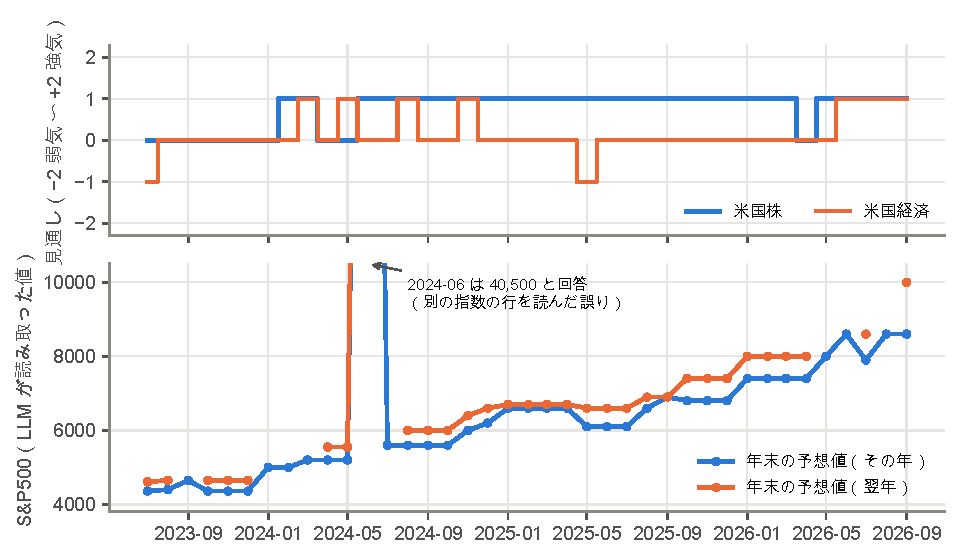
\includegraphics[width=0.84\linewidth]{reports.pdf}
\caption{LLM が月次レポートから読み取った値。上：米国株と米国経済の見通し。下：\SP{} の年末の予想値。2024 年 6 月号では、別の指数の行の値を答えている。}
\label{fig:reports}
\end{figure}

\figref{fig:reports} のとおり、米国株の見通しは 2023 年後半が中立で、2024 年以降はほぼ「やや強気」と、大きな流れは自然である。一方、\SP{} の予想値では、2024 年 6 月号で 40,500 という値を答えている。日経平均株価などの別の行を読んだ誤りである。精度の問題は \chapref{ch:expA} でくわしく見る。

月ごとの読み取り結果は、付録~\ref{app:monthly} の表にある。

\section{セクターの文章が足りない}

このレポートは世界全体の見通しで、米国のセクターにはほとんど触れていない。39 本のうち、見通しが読み取れたのは、最も多い情報技術で 10 本、ほかは 1〜6 本だった。セクターについては、数値の指標を自分で作ることにした（次の章）。

\chapter{セクターの指標}\label{ch:sector}

\section{ねらい}

運用会社が公表している「セクター・スコアカード」は、11 のセクターそれぞれに、割安さ、株価の勢い、業績の見通しの変化の点数を付けたものである。入力として理想的だが、手に入ったのは 7 か月分だけで、公表も翌月の 10 日ごろと遅い。そこで、同じ種類の指標をデータベースのデータから自分で計算し、手元の 7 本で答え合わせをすることにした（答え合わせは \chapref{ch:expB}）。

\section{何が無料で取れるか}

セクターの情報源として、セクター別の ETF と、そのオプションを調べた。yfinance で実際に確かめた結果は次のとおりである。

\begin{longtable}{p{5.60cm}p{2.40cm}p{6.40cm}}
\toprule
\textbf{データ} & \textbf{取れるか} & \textbf{確かめた内容} \\
\midrule
\endfirsthead
\toprule
\textbf{データ} & \textbf{取れるか} & \textbf{確かめた内容} \\
\midrule
\endhead
\bottomrule
\endfoot
セクター ETF 11 本の日次の株価 & 取れる & 2023 年 1 月〜2026 年 9 月の 939 日分、欠けなし \\
セクター ETF のオプション & 今日の分だけ & 満期の一覧は出るが、過去の日付の価格は取れない \\
オプションの予想変動率 & 使えない & 今日の分ですら、値が 0.00001 と壊れている行があった \\
セクター別の変動率の指数 & 取れない & エネルギーの指数などは、データが返らない \\
市場全体の変動率の指数 & 取れる & \code{\textasciicircum VIX}、\code{\textasciicircum VIX3M}、\code{\textasciicircum VIX9D}、\code{\textasciicircum SKEW}、\code{\textasciicircum VVIX} などが全期間ある \\
ETF の PER、PBR & 今日の値だけ & 過去の値は取れない \\
\end{longtable}

オプションは「今この瞬間の値」しか公開されておらず、2024 年 4 月時点の値をさかのぼって取る方法がない。そのため、セクター別の予想変動率、空売りの残高、プットとコールの比率は使わないことにした。代わりに、市場全体の \code{\textasciicircum VIX}、\code{\textasciicircum VIX3M}、\code{\textasciicircum SKEW} をデータベースに足した。

\section{指標の定義}

セクターの値動きには、Select Sector SPDR の ETF 11 本（XLC、XLY、XLP、XLE、XLF、XLV、XLI、XLK、XLB、XLRE、XLU）を使う。11 本は GICS の 11 セクターにそのまま対応する。

\begin{longtable}{p{3.60cm}p{7.60cm}p{3.20cm}}
\toprule
\textbf{指標} & \textbf{定義} & \textbf{元のデータ} \\
\midrule
\endfirsthead
\toprule
\textbf{指標} & \textbf{定義} & \textbf{元のデータ} \\
\midrule
\endhead
\bottomrule
\endfoot
\code{momentum\_3m}、\code{momentum\_6m}、\code{momentum\_12m} & 3・6・12 か月のリターン。直近の 1 か月は除く（1 か月前の月末までの値動き） & セクター ETF の株価 \\
\code{volatility\_30d} & 過去 30 取引日の日次リターンの標準偏差を年率にした値。直近 5 日の平均 & セクター ETF の株価 \\
\code{pe\_trailing} & セクターの銘柄の時価総額の合計 $\div$ 直近 4 四半期の純利益の合計 & 財務諸表、時価総額 \\
\code{pb} & 時価総額の合計 $\div$ 直近の四半期の純資産の合計 & 同上 \\
\code{ps} & 時価総額の合計 $\div$ 直近 4 四半期の売上高の合計 & 同上 \\
\code{valuation\_coverage} & セクターの時価総額のうち、\code{pe\_trailing} の計算に使えた銘柄の割合 & --- \\
\end{longtable}

\begin{itemize}
\item \textbf{モメンタムから直近 1 か月を除く}のは、短期のリターンは反転しやすいことが知られているためである。数え方は、スコアカードとの照合で決めた（\chapref{ch:expB}）。
\item \textbf{割安さの指標は ETF からではなく、構成銘柄の合算で作る。}ETF の PER は今日の値しかないためである。財務データは、判断日までに提出された四半期だけを使う。
\item 12 か月のモメンタムには 13 か月分の株価が要る。ETF だけは、ほかの銘柄より早い 2023 年 1 月から取得している。
\end{itemize}

結果はテーブル \code{sector\_metrics} に、判断日・セクター・指標ごとに 1 行で入れる。43 か月分で 3,586 行ある。ビュー \code{sector\_metric\_scores} は、同じ判断日・同じ指標の中で、各セクターが平均から標準偏差の何倍離れているか（z スコア）を付ける。

\section{計算結果の例}

\begin{table}[htbp]
\centering
\caption{2026 年 5 月 29 日のセクターの指標。かっこの中は、11 セクターの中での z スコア。}
\label{tab:sectorex}
{\footnotesize
\resizebox{\linewidth}{!}{%
\begin{tabular}{lrrrrrrr}
\toprule
セクター & モメンタム 3 か月 & 6 か月 & 12 か月 & ボラティリティ & PER & PBR & PSR \\
\midrule
Communication Services & -0.027 (-1.03) & +0.021 (-0.75) & +0.236 (-0.02) & 0.121 (-1.07) & 15.6 (-1.52) & 4.3 (-0.32) & 4.2 (+0.18) \\
Consumer Discretionary & -0.021 (-0.95) & -0.010 (-1.04) & +0.209 (-0.19) & 0.166 (-0.05) & 37.7 (+1.26) & 9.0 (+0.98) & 3.2 (-0.21) \\
Consumer Staples & +0.015 (-0.40) & +0.120 (+0.18) & +0.059 (-1.12) & 0.134 (-0.77) & 30.6 (+0.36) & 6.8 (+0.36) & 1.6 (-0.83) \\
Energy & +0.176 (+2.02) & +0.374 (+2.56) & +0.530 (+1.80) & 0.266 (+2.17) & 21.4 (-0.79) & 2.4 (-0.86) & 1.7 (-0.79) \\
Financials & -0.019 (-0.92) & +0.004 (-0.91) & +0.086 (-0.96) & 0.106 (-1.40) & 15.8 (-1.50) & 2.2 (-0.92) & 3.3 (-0.17) \\
Health Care & -0.053 (-1.42) & +0.021 (-0.75) & +0.058 (-1.13) & 0.146 (-0.50) & 28.9 (+0.15) & 4.9 (-0.17) & 1.5 (-0.86) \\
Industrials & +0.058 (+0.25) & +0.133 (+0.30) & +0.348 (+0.67) & 0.191 (+0.50) & 29.8 (+0.26) & 7.3 (+0.48) & 3.0 (-0.27) \\
Information Technology & +0.110 (+1.02) & +0.064 (-0.35) & +0.528 (+1.79) & 0.227 (+1.30) & 39.8 (+1.52) & 14.7 (+2.54) & 10.7 (+2.68) \\
Materials & +0.049 (+0.11) & +0.213 (+1.05) & +0.251 (+0.07) & 0.177 (+0.17) & 29.4 (+0.22) & 3.4 (-0.59) & 2.4 (-0.51) \\
Real Estate & +0.079 (+0.56) & +0.105 (+0.03) & +0.112 (-0.79) & 0.143 (-0.58) & 35.1 (+0.93) & 3.3 (-0.61) & 6.6 (+1.10) \\
Utilities & +0.091 (+0.74) & +0.067 (-0.32) & +0.221 (-0.11) & 0.179 (+0.23) & 20.6 (-0.89) & 2.3 (-0.89) & 2.9 (-0.33) \\
\bottomrule
\end{tabular}}
}
\end{table}

\begin{figure}[htbp]
\centering
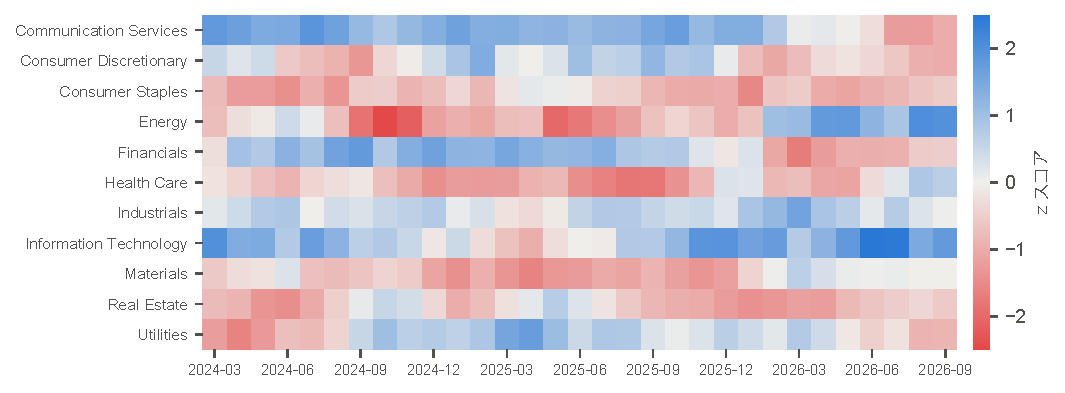
\includegraphics[width=\linewidth]{sector_momentum.pdf}
\caption{12 か月のモメンタムの z スコアの推移。青は 11 セクターの平均より強く、赤は弱い。}
\label{fig:sectormom}
\end{figure}

\section{「株式」の判定を変えた}

ETF を銘柄の一覧に足したことで、既存の処理に手を入れる必要が出た。それまでは「\code{\textasciicircum} で始まらないティッカー」を株式として扱っていた。そのままでは、ETF に対して発行済み株式数や財務諸表を取りに行ってしまう。4 か所を「指数の在籍期間がある銘柄」に変えた。対象は、変更の前と同じ 568 銘柄である。

\chapter{銘柄の指標}\label{ch:stock}

LLM に渡す入力と、比べる相手の統計モデルに入れる変数を、同じテーブルから取れるようにするため、銘柄ごとの指標を計算してデータベースに入れた。入力が同じでなければ、LLM と統計モデルの差が「モデルの差」なのか「入力の差」なのか分けられないからである。

\section{指標の定義}

指標は 14 種類ある。値動きが 5 つ、財務が 7 つ、決算の新しさが 2 つである。

\begin{longtable}{p{4.20cm}p{7.40cm}p{2.80cm}}
\toprule
\textbf{指標} & \textbf{定義} & \textbf{元のデータ} \\
\midrule
\endfirsthead
\toprule
\textbf{指標} & \textbf{定義} & \textbf{元のデータ} \\
\midrule
\endhead
\bottomrule
\endfoot
\code{momentum\_12m} & 252 取引日前から 21 取引日前までのリターン（直近 1 か月は除く） & 株価 \\
\code{return\_1m} & 直近 21 取引日のリターン & 株価 \\
\code{relative\_momentum\_12m} & \code{momentum\_12m} から、セクター ETF の同じ期間のリターンを引いた値 & 株価 \\
\code{volatility\_30d} & 過去 30 取引日の日次リターンの標準偏差を年率にした値。直近 5 日の平均 & 株価 \\
\code{beta\_1y} & 過去 252 取引日の日次リターンを \SP{} に回帰した傾き。半年分に満たなければ作らない & 株価 \\
\code{pe\_trailing} & 時価総額 $\div$ 直近 4 四半期の純利益。赤字なら作らない & 財務諸表、時価総額 \\
\code{pb} & 時価総額 $\div$ 純資産 & 同上 \\
\code{revenue\_growth\_yoy}、\code{net\_income\_growth\_yoy} & 直近の四半期 $\div$ 1 年前の同じ四半期 $- 1$。1 年前が 0 以下なら作らない & 財務諸表 \\
\code{net\_margin} & 直近 4 四半期の純利益 $\div$ 売上高 & 財務諸表 \\
\code{roe} & 直近 4 四半期の純利益 $\div$ 純資産 & 財務諸表 \\
\code{debt\_to\_equity} & 長期負債 $\div$ 純資産 & 財務諸表 \\
\code{fundamentals\_age\_days} & 使った四半期の期末から判断日までの日数 & 財務諸表 \\
\code{filing\_age\_days} & その決算の提出日から判断日までの日数 & 財務諸表 \\
\end{longtable}

銘柄の株価はデータベースに 2023 年 3 月からしかない。月の単位で数えると最初の判断日に 1 日分足りないので、モメンタムは取引日で数えている。セクターとの差も、ETF を同じ数え方で計算して引いている。

結果はテーブル \code{stock\_metrics} に、判断日・銘柄・指標ごとに 1 行で入れる。43 か月分で 256,037 行ある。計算できない指標は、行を作らない（指標ごとの行数は付録~\ref{app:monthly}）。プロンプトでは「n/a」として渡す。0 で埋めると、LLM が本当の 0 と区別できないためである。

\section{決算が古い銘柄の扱い}

判断日に使える最新の決算が、ふつうより古い銘柄がある。実測（\chapref{ch:expC}）にもとづいて、次の決まりにした。

\begin{keybox}[決まり]
使う四半期の期末から判断日までが 150 日を超える銘柄は、財務の指標をすべて作らない。日数は \code{.env} の \code{FUNDAMENTALS\_MAX\_AGE\_DAYS} で変えられる。
\end{keybox}

150 日は、「期末から提出まで最大約 2 か月 $+$ 次の四半期まで 3 か月」に当たる。これを超えるのは、次の決算が出るはずの時期を過ぎても出ていない状態である。原因が提出の遅れでも、データの欠けでも、古い数字を「最新」として渡すことを避けられる。銘柄そのものは対象から外さないので、ほかの実行と同じ銘柄で比べられる。

\section{業種によって意味が変わる指標}

業種の性質のせいで誤解を招く指標は、その業種では作らない。決まりは、GICS のサブ業種の単位で定めている。

\begin{longtable}{p{4.60cm}p{4.20cm}p{5.60cm}}
\toprule
\textbf{業種} & \textbf{作らない指標} & \textbf{理由} \\
\midrule
\endfirsthead
\toprule
\textbf{業種} & \textbf{作らない指標} & \textbf{理由} \\
\midrule
\endhead
\bottomrule
\endfoot
銀行、消費者金融、証券、資産運用・カストディ銀行 & 純利益率、負債の重さ & 借り入れ（預金）が商売の材料で、売上高も利息を差し引いた形で報告される \\
不動産投資信託（REIT、12 業種） & PER、純利益の前年同期比、純利益率、ROE & 建物の減価償却と物件の売却益で、純利益が稼ぎを表さない。業界は FFO という別の指標を使うが、データベースにない \\
複合持株会社（Berkshire Hathaway） & PER、純利益の前年同期比、純利益率、ROE & 保有株の含み損益が純利益に入る \\
\end{longtable}

同じセクターでも、決済会社、取引所、保険、不動産サービスは、すべての指標を作る。REIT の判断はデータでも確かめた。外す前は、不動産セクターの PER の中央値が 37.8 でセクター中もっとも高く、100 を超える行が 139 件、純利益率が 100\% を超える行が 31 件あった。外した後は、純利益率が 100\% を超える行は全体で 0 件である。

LLM が業種の事情を理解して数字を割り引くなら、外す必要はない。実際にどうかは実験 D（\chapref{ch:expD}）で確かめ、割り引いている証拠はなかったので、外したままにしている。

次のものは、業種の性質ではないので手を入れていない。

\begin{itemize}
\item 自社株買いで純資産が極端に小さい会社。ROE が 100\% を超える行や、PBR が 50 を超える行がある。
\item 電力会社の負債の重さ（中央値 1.53）。規制業種として自然な水準で、セクターの中の順位で見れば比べられる。
\item 資産運用会社の純利益率。本来は意味があるが、GICS がカストディ銀行と同じ業種にまとめているので、一括して外している。
\end{itemize}

\section{セクターの中での順位}

「PER 32」だけでは、高いか安いか判断しにくい。ビュー \code{stock\_metric\_scores} は、同じ判断日・同じ指標・同じセクターの銘柄の中での位置（0 が最も小さい値、100 が最も大きい値）を付ける。その指標を持つ銘柄がセクターに 5 つ未満なら、順位は付けない。REIT を外した後の不動産セクターの PER のように、比べる相手が 2 銘柄しかない場合があるためである。

\section{計算結果の例}

\begin{table}[htbp]
\centering
\caption{2026 年 5 月 29 日の指標の例。かっこの中は、セクターの中での百分位。n/a は、作らない決まりの指標である。}
\label{tab:stockex}
{\small
\begin{tabular}{lrrrr}
\toprule
指標 & NVDA（半導体） & JPM（銀行） & PLD（REIT） & XOM（石油） \\
\midrule
\texttt{momentum\_\allowbreak{}12m} & 0.504 (63) & 0.193 (69) & 0.315 (89) & 0.544 (60) \\
\texttt{return\_\allowbreak{}1m} & 0.00903 (23) & -0.0321 (34) & 0.0335 (68) & -0.0545 (50) \\
\texttt{relative\_\allowbreak{}momentum\_\allowbreak{}12m} & 0.122 (63) & 0.156 (69) & 0.232 (89) & 0.0624 (60) \\
\texttt{volatility\_\allowbreak{}30d} & 0.389 (20) & 0.207 (24) & 0.196 (21) & 0.315 (40) \\
\texttt{beta\_\allowbreak{}1y} & 1.79 (66) & 1.01 (64) & 0.64 (79) & -0.387 (10) \\
\texttt{pe\_\allowbreak{}trailing} & 32 (42) & 13.6 (45) & n/a & 23.8 (70) \\
\texttt{pb} & 26.2 (79) & 2.2 (58) & 2.5 (48) & 2.37 (50) \\
\texttt{revenue\_\allowbreak{}growth\_\allowbreak{}yoy} & 0.852 (93) & 0.0999 (49) & 0.0739 (57) & 0.0242 (37) \\
\texttt{net\_\allowbreak{}income\_\allowbreak{}growth\_\allowbreak{}yoy} & 2.11 (82) & 0.126 (34) & n/a & -0.458 (18) \\
\texttt{net\_\allowbreak{}margin} & 0.63 (100) & n/a & n/a & 0.0757 (32) \\
\texttt{roe} & 0.817 (89) & 0.162 (58) & n/a & 0.0995 (10) \\
\texttt{debt\_\allowbreak{}to\_\allowbreak{}equity} & 0.0382 (13) & n/a & 0.648 (33) & n/a \\
\texttt{fundamentals\_\allowbreak{}age\_\allowbreak{}days} & 33 (10) & 59 (0) & 59 (0) & 59 (0) \\
\texttt{filing\_\allowbreak{}age\_\allowbreak{}days} & 9 (11) & 28 (51) & 29 (46) & 25 (45) \\
\bottomrule
\end{tabular}
}
\end{table}

\section{分かっている問題}

\begin{itemize}
\item \textbf{負債の重さは、約半分の銘柄にしか値がない。}長期負債の項目名が会社によって違い、ビューが拾えていない。
\item \textbf{2026 年 8 月末と 9 月末は、約 12\% の銘柄で財務の指標がない。}2026 年 4〜6 月期の決算が、57 銘柄で元のデータにないためである。ほかの月は、多くても 2\% である。
\item \textbf{極端な値がある。}たとえば SanDisk の 12 か月のモメンタムは $+2{,}657\%$ である。株価そのものがそう動いていて、計算の誤りではない。
\end{itemize}

\chapter{予測用プロンプトの入出力の設計}\label{ch:io}

各銘柄の翌月のリターンを予測させる LLM に、何を渡して何を受け取るかの設計をまとめる。この設計は実験の前に立てたもので、実験の結果（第 V 部）を受けて見直すべき点を、章の最後に書く。

\section{入力のまとまり}

入力を 6 つのまとまりに分ける。まとまりごとに入れる・入れないを切り替えられるようにし、どれが効いたかを後で測る。

\begin{longtable}{p{3.40cm}p{5.40cm}p{2.60cm}p{3.00cm}}
\toprule
\textbf{まとまり} & \textbf{中身} & \textbf{値が変わる単位} & \textbf{状態} \\
\midrule
\endfirsthead
\toprule
\textbf{まとまり} & \textbf{中身} & \textbf{値が変わる単位} & \textbf{状態} \\
\midrule
\endhead
\bottomrule
\endfoot
A　銘柄の基本情報 & ティッカー、社名、セクター、サブ業種 & 銘柄 & 使用中 \\
B　値動き & モメンタム、直近のリターン、ボラティリティ、ベータ & 銘柄 $\times$ 月 & 計算済み \\
C　ファンダメンタルズ & 割安さ、成長、収益性、負債 & 銘柄 $\times$ 月 & 計算済み \\
D　セクター & セクターのモメンタム、ボラティリティ、PER & セクター $\times$ 月 & 計算済み \\
E　市場全体 & VIX、VIX の期間構造、SKEW、短期金利 & 月 & データあり \\
F　レポートの文章 & 米国の見通しの要約、主なリスク & 月 & 抽出済み \\
\end{longtable}

今の実装（実行番号 1）は、A と「1 か月分の日次リターン（約 20 個）」だけを渡している。日次リターンの列は、LLM が数字をなぞる原因になっているので、B の要約に置き換える。

\subsection{数字の渡し方}

\begin{itemize}
\item \textbf{セクターの中の順位を添える。}銘柄ごとの数字（B と C）には、同じセクターの中での百分位を付ける。
\item \textbf{単位をプロンプトに書く。}リターンは小数、VIX と金利はパーセント、と明記する。
\item \textbf{欠けている数字は「n/a」と渡す。}
\item \textbf{桁数をそろえる。}有効数字 3 桁程度に丸める。
\item \textbf{決算の日付を添える。}「どの四半期の決算か」と「提出日」を渡す。
\end{itemize}

\section{未来の情報を使わない決まり}

\begin{longtable}{p{3.00cm}p{6.20cm}p{5.20cm}}
\toprule
\textbf{まとまり} & \textbf{使ってよい範囲} & \textbf{確かめ方} \\
\midrule
\endfirsthead
\bottomrule
\endfoot
A　基本情報 & 判断日に指数に在籍していた銘柄だけ & 在籍期間のテーブル \\
B　値動き & 判断日までの株価 & 株価の日付が判断日以前 \\
C　ファンダ & 判断日までに提出された四半期だけ & 提出日が判断日以前 \\
D　セクター & 判断日までの ETF の株価と、提出済みの決算 & 指標の判断日 \\
E　市場 & 判断日の終値 & 株価の日付 \\
F　レポート & 判断日までに公表されたレポートのうち、最新の 1 本 & 公表日が判断日以前 \\
モデルの知識 & 知識が 2023 年 10 月までの gpt-4o-mini を使い、評価は 2024 年 4 月から & 実行の記録にあるモデルの版 \\
\end{longtable}

\section{プロンプトの形}

まとまりごとに見出しを付けて並べる。使わないまとまりは、見出しごと省く。実験 D で実際に使ったプロンプト（まとまり A、B、C）の形は、リスト~\ref{lst:io} のとおりである。

\begin{lstlisting}[caption={プロンプトの形（値は省略。かっこの中はセクターの中での百分位）},label={lst:io}]
[Stock]
Ticker: PLD
Security: Prologis
Sector: Real Estate
Sub-Industry: Industrial REITs

[Price behaviour]  (value, percentile in sector)
12-month momentum, latest month excluded: ...
Return over the latest month: ...
12-month momentum minus the sector's: ...
30-day volatility, per year: ...
Beta to the S&P 500: ...

[Fundamentals]  quarter ended YYYY-MM-DD, filed YYYY-MM-DD  (value, percentile in sector)
Price / earnings, last 4 quarters: ...
Price / book: ...
Revenue growth, year on year: ...
Net income growth, year on year: ...
Net margin: ...
Return on equity: ...
Long-term debt / equity: ...
\end{lstlisting}

数字を入れた実物は、付録~\ref{app:prompts} のリスト~\ref{lst:expD} にある。セクター、市場、レポートを足す場合は、この後ろに \code{[Sector: ...]}、\code{[Market]}、\code{[Monthly outlook of an asset manager, published ...]} のまとまりを足す（実験 F と G で使った形）。

\section{出力}

\begin{longtable}{p{3.60cm}p{10.80cm}}
\toprule
\textbf{項目} & \textbf{内容} \\
\midrule
\endfirsthead
\bottomrule
\endfoot
回答の形 & JSON で \code{\{"expected\_return": 数値\}}。API の機能で固定する \\
回答の意味 & 翌月の日次の平均リターン（小数） \\
回答の数 & 1 銘柄・1 か月につき 30 個。1 回のリクエストで受け取る \\
ばらつき & temperature は 1.0。0 にすると 30 個が同じ答えになり、分散が出ない \\
読み取れなかった回答 & 空の値として保存し、平均と分散の計算から外す \\
理由の文章 & 出させない。30 個すべてに文章が付くと、出力の費用が数十倍になる \\
\end{longtable}

\section{実行の条件}

まとまりを 1 つずつ足して実行し、どれが効いたかを測る計画である。

\begin{longtable}{rp{4.20cm}p{7.00cm}p{2.20cm}}
\toprule
 & \textbf{入力} & \textbf{確かめること} & \textbf{状態} \\
\midrule
\endfirsthead
\bottomrule
\endfoot
1 & A $+$ 日次リターンの列 & 既存手法の再現 & 済み \\
2 & A $+$ B & 日次リターンの列を要約に置き換えると、なぞりが減るか & 小規模に実験 \\
3 & A $+$ B $+$ C & ファンダを足した効果 & 小規模に実験 \\
4 & A〜E & セクターと市場を足した効果 & 未実施 \\
5 & A〜F & レポートの文章を足した効果 & 未実施 \\
\end{longtable}

実行 1 は、全期間で約 1.75 ドルだった。入力が 2 倍強になっても、1 回 3〜4 ドル程度の見込みである。

\section{実験を受けて見直す点}

この設計のうち、実行 2 と 3 に当たる部分は、実験 D〜F で小さな規模で試した。その結果、設計の前提のいくつかが成り立たないことが分かった。

\begin{itemize}
\item \textbf{日次リターンの列を要約に置き換えても、なぞりは減らなかった。}予想は、直近 1 か月のリターンとの順位相関が $+0.5$ 前後あった。
\item \textbf{ファンダの数字は、ほとんど使われなかった。}渡しても、予想の変化は「同じ質問を 2 回したときのぶれ」と同じ程度だった。
\item \textbf{「直近 1 か月のリターンを入れるか」は、当初「入れる」としていた。}なぞりの元になっているので、外すことを検討する。
\end{itemize}

したがって、まとまりを足していく実行 4 と 5 を全期間で行う前に、質問の形そのものを決め直す必要がある。その方向は \chapref{ch:synthesis} と \chapref{ch:future} で述べる。

なお、データベースの \code{llm\_runs} には、どのまとまりを使ったかを記録する列と、ユーザープロンプトの型を記録する列がまだない。今はシステムプロンプトしか保存していないので、入力を変えた実行を全期間で行う前に足す必要がある。

% ============================================================
\part{実験}
% ============================================================

\chapter{実験の全体像}\label{ch:expall}

2026 年 10 月 13 日に、7 つの実験と確認を行った。A〜C は入力のデータを作るための確認、D〜G は予測用のプロンプトの実験である。

\begin{longtable}{cp{3.20cm}p{5.60cm}p{2.20cm}p{2.60cm}}
\toprule
 & \textbf{実験} & \textbf{確かめたこと} & \textbf{規模} & \textbf{結論} \\
\midrule
\endfirsthead
\toprule
 & \textbf{実験} & \textbf{確かめたこと} & \textbf{規模} & \textbf{結論} \\
\midrule
\endhead
\bottomrule
\endfoot
A & レポートの読み取り & gpt-4o-mini は月次レポートの数字を正しく取り出せるか & 39 本 $\times$ 24 項目 & 文章は可。表の数字は誤りが残る \\
B & セクター指標の照合 & 自作のモメンタムとボラティリティは正しいか & 7 か月 $\times$ 11 セクター & スコアカードと一致 \\
C & 決算の古さ & 判断日に使える決算は、どのくらい古いか & 14,688 件 & 150 日で線を引く \\
D & 業種の特性 & REIT や銀行の誤解を招く指標を、LLM は割り引くか & 2,067 リクエスト & 割り引く証拠なし。そもそもファンダを使わない \\
E & 比率の明言 & 「値動き何 \%、ファンダ何 \%」と指定すれば、なぞりが減るか & 714 リクエスト & 減らない。桁が壊れる \\
F & 3 ターンの会話 & 業種とセクターについて先に答えさせれば、なぞりが減るか & 957 リクエスト & なぞりは強まった \\
G & リスクプレミアムの有無 & 銘柄の数字を渡さず、リスクの種類ごとに聞くとどうなるか & 540 リクエスト & 渡した市場の数字に沿い、当たらない \\
\end{longtable}

D〜G の回答は、データベースには入れていない。スクリプトと全回答は、フォルダ \code{LLM-BLM\_実験/} にある（付録~\ref{app:files}）。

\section{実験の共通の作り}

実験 D〜F は、同じ作りを共有している。

\begin{description}[leftmargin=2em,style=nextline,itemsep=0.3em]
\item[入力] 銘柄の基本情報、値動きの指標 5 つ、財務の指標 7 つ。値と、セクターの中での百分位を渡す（\chapref{ch:io}）。指標は \code{stock\_metrics} と同じ計算で作るが、業種による除外（\chapref{ch:stock}）は実験のために外している。
\item[回答] 1 リクエストで 30 個。temperature は 1.0。30 個の平均を、その銘柄の予想とする。
\item[見る量] 判断日ごとに、銘柄の間で「予想の順位」と「指標の順位」の相関を取り、判断日について平均する。予想が何に沿って付いているかを表す。
\item[雑音の目安] 同じ質問をもう 1 回行い、予想の平均がどれだけずれるかを測る。これより小さい差は、効果とは言えない。
\end{description}

\begin{notebox}[結果を読むときの注意]
\begin{itemize}
\item 規模が小さい。D は 5 つ、E と F は 3 つの判断日だけである。傾向は読めるが、相関の細かい大小は当てにならない。
\item D〜F で見ているのは「予想が入力のどれに沿っているか」で、予想が当たったかどうかではない。当たったかどうかを見たのは、G だけである。
\item モデルは gpt-4o-mini だけである。
\end{itemize}
\end{notebox}

% ------------------------------------------------------------
\chapter{実験 A：月次レポートの読み取りの精度}\label{ch:expA}

\section{目的と方法}

月次レポート 39 本から、見通しの数字と要約を gpt-4o-mini に取り出させ（\chapref{ch:reports}）、どこまで正しいかを確かめた。

答えには、PDF の文字から決まった形で読める行を使った。新しい構成のレポート（2024 年 9 月号以降）では、\SP{} の行と GDP の行が 1 行の文字としてきれいに入っている。この行を正規表現で読み取り、LLM の回答と照らした。古い構成のレポートは文字の並びが崩れているので、答えを作れなかった。

\section{結果}

\begin{longtable}{p{5.40cm}p{2.20cm}p{6.80cm}}
\toprule
\textbf{項目} & \textbf{一致} & \textbf{補足} \\
\midrule
\endfirsthead
\bottomrule
\endfoot
米国の GDP 成長率（今年） & 16 ／ 18 & \\
米国の GDP 成長率（来年） & 15 ／ 18 & \\
\SP{} の年末の予想値（今年・来年） & 20 本中 12〜13 & 不一致のうち 4 本は、答えの側の誤りだった（次の節）。実際は 16〜17 本が正しい見込み \\
\SP{} の直近値 & 5 ／ 20 & 5 本は答えなし。ほかは別の数字を拾った \\
政策金利、米 10 年金利 & --- & 手で確かめた 2 本で誤りがあった \\
見通しの判断（弱気〜強気） & --- & 同じレポートで $-1$ と 0 に分かれた \\
\end{longtable}

\section{見つかった誤りの種類}

\begin{description}[leftmargin=2em,style=nextline,itemsep=0.4em]
\item[年の列の取り違え] 最初の版のプロンプトでは、2025 年 6 月号の GDP を 1 年ずれて読んだ（2025 年の予想 1.4\% を、2026 年のものとして答えた）。プロンプトに「何年何月号か」を入れ、項目の説明の中の年を具体的な年にして減らしたが、上の表のとおり、なくなってはいない。
\item[別の行を読む] 2024 年 6 月号では、\SP{} の予想値として 40,500 と 43,200 を答えた。別の株価指数の行を読んでいる（\figref{fig:reports}）。
\item[範囲の読み方] 政策金利は「5.25〜5.50」のような範囲で印刷されている。2023 年 7 月号では、これを 5.0 と答えた。
\item[予想値と直近値の取り違え] 2025 年 6 月号の米 10 年金利は、年末の予想値ではなく直近値を答えた。
\item[図で示された判断] 「弱気〜強気」は、表の中の印の位置で示されていて、文字としては入っていない。2025 年 6 月号の米国経済は、表では「やや弱気」（$-1$）だが、1 回目の読み取りは $-1$、プロンプトを変えた 2 回目は 0 だった。
\end{description}

\section{答えの側の誤り}

位置で決めた答えにも、誤りがあった。11 月号と 12 月号は、予想値の表に翌々年の列が加わり、列が 1 つずれる。この 4 本（2024 年 11・12 月号、2025 年 11・12 月号）では、「不一致」とされた LLM の回答のほうが正しかった。自動の答え合わせは、答えを作る側の検証も要る、という例である。

\section{結論}

\begin{itemize}
\item 予測の入力に使うのは、要約と主なリスクの文章だけにする。2 本を読んだ範囲では、レポートの内容と合っていた。
\item 表の数字を使うなら、LLM ではなく、PDF の文字から年の見出しを手がかりに取り出すべきである。LLM に読ませると、1〜2 割の誤りが混ざる。
\item 政策金利と 10 年金利は、文字の並びが崩れていて機械的に取るのも難しい。項目から外すのが現実的である。金利の水準は、市場のデータ（\code{\textasciicircum IRX}）から取れる。
\end{itemize}

% ------------------------------------------------------------
\chapter{実験 B：セクターの指標とスコアカードの照合}\label{ch:expB}

\section{目的と方法}

セクター ETF の株価から自作したモメンタムとボラティリティ（\chapref{ch:sector}）が、運用会社の公表値と合うかを確かめた。

相手は、ステート・ストリートの「米国株式セクター スコアカード」7 本である。データの時点は 2026 年 2 月末から 8 月末までの 7 か月で、PDF の作成日は、それぞれ翌月の 7〜12 日だった。表の数字は PDF に文字として入っているので、行ごとに読み取った。同じ判断日の自作の指標と、11 セクターの間の相関を取った。

\section{結果}

\begin{figure}[htbp]
\centering
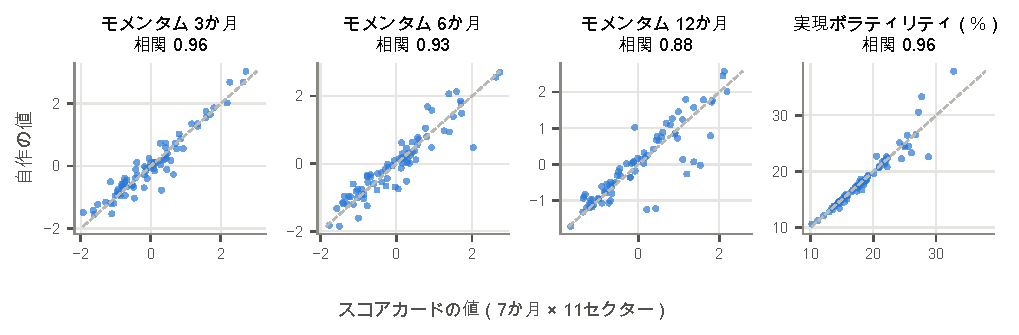
\includegraphics[width=\linewidth]{scorecard.pdf}
\caption{スコアカードの値（横軸）と自作の値（縦軸）。点は、判断日 $\times$ セクター。モメンタムは z スコア、ボラティリティは年率のパーセント。}
\label{fig:scorecard}
\end{figure}

\begin{table}[htbp]
\centering
\caption{スコアカードとの相関（判断日ごとに計算して、7 か月を平均）。}
\small
\begin{tabular}{lrl}
\toprule
指標 & 相関 & 判定 \\
\midrule
モメンタム 3 か月 & 0.96 & 一致 \\
モメンタム 6 か月 & 0.93 & 一致 \\
モメンタム 12 か月 & 0.88 & ほぼ一致 \\
モメンタムの総合（3 つの z スコアの平均） & 0.93 & 一致 \\
実現ボラティリティ（水準の比は 0.99） & 0.97 & 一致 \\
実現ボラティリティと、スコアカードの予想ボラティリティ & 0.83 & 大まかには代用できる \\
PER、PBR、PSR（順位相関） & 0.08〜0.39 & 一致しない \\
\bottomrule
\end{tabular}
\end{table}

\section{モメンタムの数え方}

スコアカードには「モメンタムの計測では直近 1 か月のデータを除外している」とあるが、正確な数え方は書かれていない。3 通りを試し、最も合ったものを採用した。

\begin{table}[htbp]
\centering
\caption{数え方ごとの、スコアカードとの相関（7 か月の平均）。$n$ は 3、6、12。}
\small
\begin{tabular}{lrrr}
\toprule
数え方 & 3 か月 & 6 か月 & 12 か月 \\
\midrule
直近の $n$ か月（除外なし） & 0.62 & 0.69 & 0.76 \\
$n$ か月前から 1 か月前まで（期間は $n-1$ か月） & 0.81 & 0.86 & 0.84 \\
$n+1$ か月前から 1 か月前まで（期間は $n$ か月）\textbf{：採用} & 0.96 & 0.93 & 0.88 \\
\bottomrule
\end{tabular}
\end{table}

ボラティリティは、「過去 30 取引日の標準偏差を年率にし、直近 5 日で平均する」が最も合った（21 取引日では 0.92、30 取引日では 0.97）。

\section{割安さが一致しない理由}

スコアカードの割安さの点数は、「そのセクター自身の過去 15 年と比べて割安か」を表している。データベースの財務データは 2021 年からなので、同じ計算はできない。データベースにあるのは「今の PER そのもの」で、別の指標である。計算そのものは正しく動いていて、2026 年 5 月末の PER は情報技術が 39.8、金融が 15.8 だった。

\section{結論}

モメンタムとボラティリティは、自作の値をそのまま使える。スコアカードそのものは、7 か月分しかなく公表も遅いので、予測の入力には使わない。

% ------------------------------------------------------------
\chapter{実験 C：決算の古さの実測}\label{ch:expC}

\section{目的と方法}

判断日に使える最新の決算が、どのくらい古いことがあるかを測り、「古すぎる」の線を決めた。評価する 30 か月 $\times$ 構成銘柄（14,688 件）について、判断日までに提出された最新の四半期を調べた。

\section{結果}

\begin{figure}[htbp]
\centering
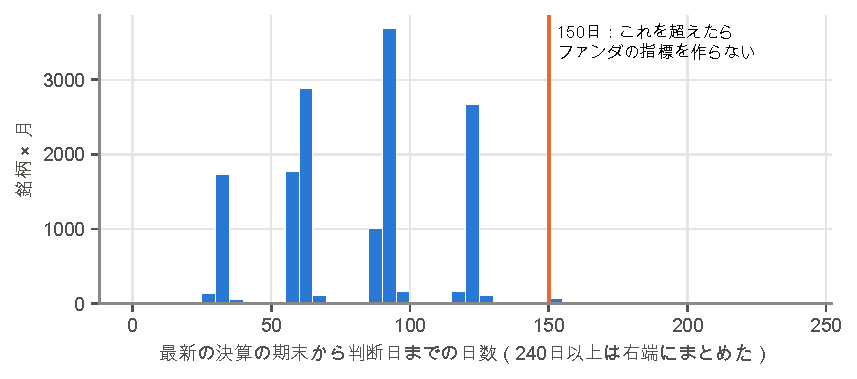
\includegraphics[width=0.9\linewidth]{filing_age.pdf}
\caption{最新の決算の期末から判断日までの日数の分布（不具合を直した後のデータ）。約 30 日ごとに山があるのは、判断日が月末で、決算期末も月末に集まっているためである。}
\label{fig:age}
\end{figure}

\begin{table}[htbp]
\centering
\caption{決算の古さ。「直す前」は、提出日の不具合を直す前の値である。}
\small
\begin{tabular}{lrr}
\toprule
 & 直す前 & 直した後 \\
\midrule
期末から判断日までの日数（中央の値） & 89 日 & 89 日 \\
同（95\% がこの範囲） & 123 日以内 & 123 日以内 \\
同（99\% がこの範囲） & 152 日以内 & 126 日以内 \\
同（最大） & 487 日 & 368 日 \\
150 日を超える件数 & 165 件（1.1\%） & 95 件（0.6\%） \\
\bottomrule
\end{tabular}
\end{table}

ふつうは、四半期が終わって約 1 か月後に決算が提出され、その 3 か月後に次の決算が出る。したがって、古さには上限がある。150 日を超えるのは、次の決算が出るはずの時期を過ぎても出ていない状態である。原因は 2 種類あった。

\begin{itemize}
\item \textbf{実際に提出が遅れた会社}：Super Micro Computer（2024 年 9 月〜2025 年 1 月）、Trimble、Autodesk は、年次報告書の提出が遅れた時期と一致する。
\item \textbf{データの側の問題}：次の節で述べる。
\end{itemize}

\section{見つけて直した不具合}

APA という会社は、古さが最大 487 日と出ていた。調べると、決算が遅れたのではなく、提出日が実際より約 1 年遅く記録されていた。

原因は、四半期の値を選ぶビューにあった。同じ四半期の純利益に 2 種類の項目名（\code{NetIncomeLoss} と \code{ProfitLoss}）があるとき、ビューは優先順位の高い項目を選んでいた。APA の 2024 年 4〜6 月期では、当時の報告書に載っていたのは優先順位の低い項目だけで、優先順位の高い項目は、翌年の報告書に比較用として初めて載った。そのため、翌年の提出日（2025-08-07）が選ばれていた。正しくは 2024-08-02 である。

「最初に提出された値を優先する」に変えた。これは、「その時点で知られていた数字を使う」という決まりに合う。影響は、11,168 の四半期のうち、提出日が変わったものが 60 件、純利益の値が変わったものが 100 件だった。変わった値を調べると、直した後のほうが正しかった。たとえば American Electric Power の 2022 年 7〜9 月期は、直す前は後の報告書の誤った値（1 つ前の四半期と同じ数字）を拾っていた。

\section{直せなかった欠け}

2026 年 4〜6 月期の決算が、57 銘柄でデータベースにない。Abbott、Visa、電力会社の多くなどである。EDGAR にもう一度問い合わせて確かめたが、返ってくるデータ自体に入っていなかった。取得の誤りではなく、元のデータの欠けである。このため、2026 年 8 月末と 9 月末は、約 12\% の銘柄で財務の指標が空になる。

\section{結論}

決算期末から 150 日を超えた銘柄は、財務の指標を作らない（\chapref{ch:stock}）。この確認は、データの不具合を 1 つ見つけることにもつながった。極端な値を「外れ値」として捨てる前に、原因を調べる価値があることを示している。

% ------------------------------------------------------------
\chapter{実験 D：LLM は業種の特性を踏まえて数字を読むか}\label{ch:expD}

\section{問い}

REIT の PER や銀行の負債のように、業種の性質で誤解を招く指標がある。LLM が業種を踏まえてそれを割り引くなら、そのまま渡しても問題はない。実際はどうかを確かめた。

\section{方法}

\begin{longtable}{p{3.20cm}p{11.20cm}}
\toprule
\textbf{項目} & \textbf{内容} \\
\midrule
\endfirsthead
\bottomrule
\endfoot
対象 & REIT（のべ 135）、銀行・証券など（160）、比較用の資本財セクター（394）。5 つの判断日（2024-06-28、2024-12-31、2025-06-30、2025-12-31、2026-05-29） \\
入力 & 銘柄の基本情報、値動きの指標 5 つ、財務の指標 7 つ \\
条件 & (1) 問題の指標を渡す　(2) n/a にする　(3) n/a でもう 1 回（雑音の目安） \\
出し入れした指標 & REIT と資本財：PER、純利益の前年同期比、純利益率、ROE。銀行：純利益率、負債の重さ \\
規模 & 2,067 リクエスト（各 30 個の回答）。失敗 0 件 \\
\end{longtable}

資本財セクターは、財務の指標がふつうに意味を持つ業種として、比べる相手に入れた。LLM が業種を踏まえて割り引いているなら、REIT では指標への反応が弱く、資本財でははっきり出るはずである。

\section{結果 1：指標を渡しても、予想はほとんど変わらない}

\begin{table}[htbp]
\centering
\caption{指標を渡したときの予想の変化と、同じ質問を 2 回したときのぶれ（日次リターンの予想の差の平均）。}
\small
\begin{tabular}{lrrr}
\toprule
業種 & 渡したときの変化 & 2 回聞いたときのぶれ & 比 \\
\midrule
REIT（4 指標を出し入れ） & 0.073\% & 0.045\% & 1.6 倍 \\
銀行・証券など（2 指標） & 0.061\% & 0.066\% & 0.9 倍 \\
資本財（4 指標、比較用） & 0.071\% & 0.057\% & 1.3 倍 \\
\bottomrule
\end{tabular}
\end{table}

銘柄の間の予想のばらつき（標準偏差）は約 0.2\% である。銀行では、指標を渡しても渡さなくても、ぶれの範囲に収まった。資本財でも、4 つの指標を渡した効果は、ぶれの 1.3 倍にとどまった。

\section{結果 2：予想を決めているのは値動き}

\begin{figure}[htbp]
\centering
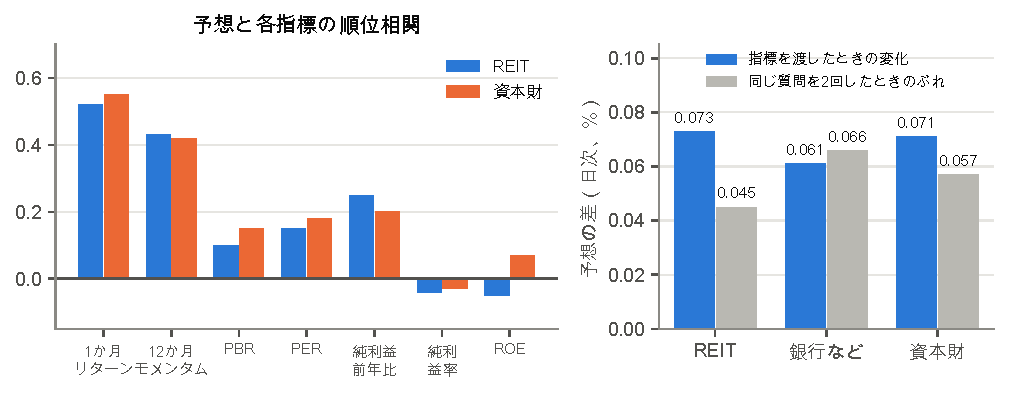
\includegraphics[width=0.92\linewidth]{exp_d.pdf}
\caption{左：予想と各指標の順位相関（指標を渡した条件）。右：指標を渡したときの予想の変化と、雑音の目安。}
\label{fig:expD}
\end{figure}

予想との順位相関は、直近 1 か月のリターンが $+0.5$ 前後、12 か月のモメンタムが $+0.4$ 前後だった（銀行では $+0.20$）。財務の指標は、高くても $+0.25$ である。日次リターンの列を要約に置き換えても、予想は値動きに沿っている。

\section{結果 3：REIT だけ反応が弱い、ということはない}

指標を渡したことで予想がどちらに動いたかを、その指標の高低と比べた。

\begin{table}[htbp]
\centering
\caption{「指標を渡したことによる予想の変化」と「その指標の高低」の順位相関。}
\small
\begin{tabular}{lrr}
\toprule
指標 & REIT & 資本財 \\
\midrule
PER & $-0.12$ & $-0.01$ \\
純利益の前年同期比 & $+0.10$ & $-0.07$ \\
純利益率 & $+0.19$ & $+0.13$ \\
ROE & $+0.08$ & $+0.05$ \\
\bottomrule
\end{tabular}
\end{table}

どちらの業種でも関係は弱く、差がない。意味が薄いはずの REIT の純利益率には、5 つの判断日すべてで同じ向きの弱い引っ張りがあった。

\section{結論}

\begin{itemize}
\item \textbf{業種を踏まえて割り引いている証拠はない。}REIT と資本財で、指標への反応に差がなかった。ただし相関はどれも小さく、「割り引いていない」と言い切れる強さではない。
\item \textbf{それ以前に、財務の数字がほとんど使われていない。}
\item \textbf{誤解を招く指標は、作らないままにする。}外して失うものがなく、統計モデルと入力をそろえられる。
\end{itemize}

% ------------------------------------------------------------
\chapter{実験 E：考慮する比率を明言する}\label{ch:expE}

\section{問い}

値動きと財務を「何 \% ずつ考慮するか」をプロンプトで明言すれば、値動きのなぞりが減り、財務が使われるか。

\section{方法}

実験 D のシステムプロンプトの末尾に、次の 1 文を足した。

\begin{lstlisting}
Weigh the two groups of information as follows when you form the prediction:
[Price behaviour] 50%, [Fundamentals] 50%.
\end{lstlisting}

対象は資本財セクターの 3 つの判断日（2025-06-30、2025-12-31、2026-05-29）、のべ 238 銘柄である。比率は「値動き：財務」を 50：50、20：80、0：100 の 3 通りにし、指定なし（実験 D の結果）と比べた。714 リクエストで、失敗は 0 件だった。

\section{結果 1：中間の比率では、なぞりは減らない}

\begin{figure}[htbp]
\centering
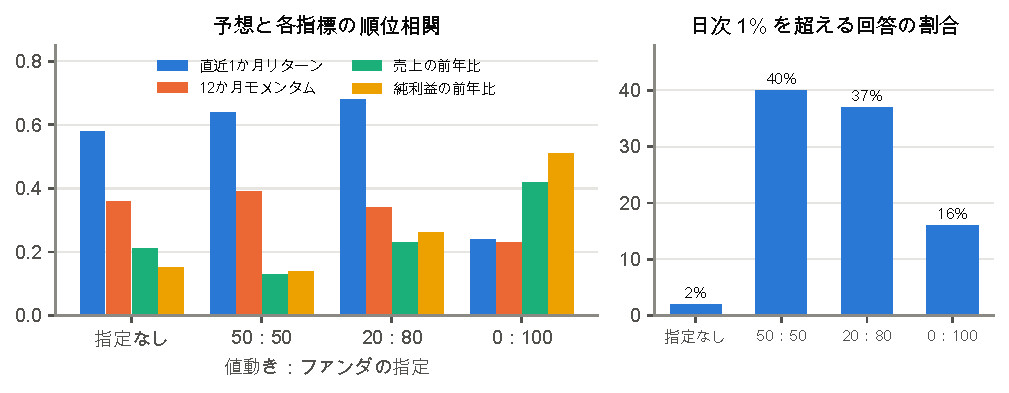
\includegraphics[width=\linewidth]{exp_e.pdf}
\caption{左：予想と各指標の順位相関。右：日次 1\% を超える回答の割合。}
\label{fig:expE}
\end{figure}

\begin{table}[htbp]
\centering
\caption{予想と各指標の順位相関（資本財、3 つの判断日の平均）。}
\small
\begin{tabular}{lrrrr}
\toprule
指標 & 指定なし & 50：50 & 20：80 & 0：100 \\
\midrule
直近 1 か月のリターン & $+0.58$ & $+0.64$ & $+0.68$ & $+0.24$ \\
12 か月のモメンタム & $+0.36$ & $+0.39$ & $+0.34$ & $+0.23$ \\
売上高の前年同期比 & $+0.21$ & $+0.13$ & $+0.23$ & $+0.42$ \\
純利益の前年同期比 & $+0.15$ & $+0.14$ & $+0.26$ & $+0.51$ \\
PER & $+0.09$ & $+0.08$ & $+0.12$ & $+0.11$ \\
PBR & $+0.11$ & $+0.09$ & $+0.09$ & $+0.05$ \\
ROE & $+0.08$ & $+0.05$ & $+0.04$ & $0.00$ \\
\bottomrule
\end{tabular}
\end{table}

\begin{itemize}
\item 「財務 80\%」と指定しても、直近 1 か月のリターンとの相関は下がらなかった（$+0.58 \to +0.68$）。
\item 0：100 でようやく値動きから離れるが、相関は $+0.24$ 残る。
\item 財務で使われるのは成長率だけである。PER、PBR、ROE は、どの条件でもほぼ使われない。
\end{itemize}

\section{結果 2：予想の桁が壊れる}

\begin{table}[htbp]
\centering
\caption{予想の大きさ（資本財、3 つの判断日）。}
\small
\begin{tabular}{lrrrr}
\toprule
 & 指定なし & 50：50 & 20：80 & 0：100 \\
\midrule
予想の平均（日次） & 0.17\% & 1.03\% & 0.70\% & 0.60\% \\
日次 1\% を超える回答の割合 & 2\% & 40\% & 37\% & 16\% \\
銘柄の間の予想のばらつき & 0.22\% & 1.90\% & 0.97\% & 1.01\% \\
30 個の回答のばらつき & 0.20\% & 1.08\% & 0.80\% & 1.07\% \\
\bottomrule
\end{tabular}
\end{table}

日次 1\% は、月に約 20\% の上昇にあたる。原因は、渡した数字をそのまま重み付きで足していることだと考えられる。たとえば Uber（2025 年 6 月末）は、直近 1 か月のリターンが 0.107、売上の前年同期比が 0.138 だった。50：50 での回答は 0.10〜0.16 に集まっていて、この 2 つを足して割った値とほぼ同じである。

\section{結論}

比率の明言は採用しない。「重み」が、判断の重みではなく計算の重みとして受け取られ、Black-Litterman に入れられる予想にならない。この実験から、gpt-4o-mini は渡した数字を「予想の材料」ではなく「答えの元」として扱う、という見方が出てきた。リターンを渡せばリターンをなぞり、成長率だけを渡せば成長率をなぞる。

% ------------------------------------------------------------
\chapter{実験 F：3 ターンの会話にしてから数字を聞く}\label{ch:expF}

\section{問い}

実験 D と E から、gpt-4o-mini は業種の知識を持っていても、数字の表から数字を 1 つ返す形では使っていない、と考えられた。そこで、2 つを確かめた。

\begin{itemize}
\item \textbf{会話にする効果}：先に業種とセクターについて文章で答えさせれば、その内容を踏まえて予想するようになるか。
\item \textbf{答えの形を変える効果}：数字ではなく 5 段階で答えさせれば、入力の数字をそのまま足すことができなくなり、なぞりが減るか。
\end{itemize}

\section{方法}

\begin{figure}[htbp]
\centering
\begin{tikzpicture}[x=10mm,y=10mm]
\node[box=c1,minimum width=40mm] (q1) at (0,0) {ターン 1 の質問\\{\scriptsize この業種で、どの指標が意味を持つか}};
\node[box=c4,minimum width=40mm] (a1) at (4.6,0) {回答（80 語以内）\\{\scriptsize 業種ごとに 1 つ。32 通り}};
\node[box=c1,minimum width=40mm] (q2) at (0,-1.5) {ターン 2 の質問\\{\scriptsize セクター・市場・レポートを渡す}};
\node[box=c4,minimum width=40mm] (a2) at (4.6,-1.5) {回答（80 語以内）\\{\scriptsize 業種 $\times$ 月。96 通り}};
\node[box=c1,minimum width=40mm] (q3) at (0,-3.0) {ターン 3 の質問\\{\scriptsize 銘柄のデータを渡す}};
\node[box=c2,minimum width=40mm] (a3) at (4.6,-3.0) {回答（30 個）\\{\scriptsize 数字、または 5 段階}};
\draw[arr] (q1) -- (a1);
\draw[arr] (q2) -- (a2);
\draw[arr] (q3) -- (a3);
\draw[arr] (a1.south west) -- (q2.north east);
\draw[arr] (a2.south west) -- (q3.north east);
\node[lab,anchor=west] at (7.0,0) {1 回作って使い回す};
\node[lab,anchor=west] at (7.0,-1.5) {1 回作って使い回す};
\node[lab,anchor=west] at (7.0,-3.0) {銘柄ごとに聞く};
\end{tikzpicture}
\caption{3 ターンの会話の作り。API は会話を覚えていないので、ターン 1 と 2 の質問と回答は、ターン 3 のリクエストに含めて送る。}
\label{fig:turns}
\end{figure}

\begin{longtable}{p{3.20cm}p{11.20cm}}
\toprule
\textbf{項目} & \textbf{内容} \\
\midrule
\endfirsthead
\bottomrule
\endfoot
対象 & 資本財セクター（のべ 238）と REIT（81）。3 つの判断日、のべ 319 銘柄 \\
条件 & (1) 1 ターン・数字（実験 D の結果を使う）　(2) 3 ターン・数字　(3) 1 ターン・5 段階　(4) 3 ターン・5 段階 \\
5 段階の問い & 「同じセクターのほかの銘柄と比べた翌月のリターン」を、$-2$（かなり低い）から $+2$（かなり高い）で答える \\
ターン 1、2 の回答 & temperature を 0 にして 1 回だけ作り、同じ業種・同じ月の全銘柄で使い回した \\
規模 & 新しく送ったのは 957 リクエスト。失敗 0 件、読み取れない回答 0 個 \\
\end{longtable}

質問と回答の実例は、付録~\ref{app:prompts} のリスト~\ref{lst:expF} にある。ターン 1 の回答の全文（32 業種）は、付録~\ref{app:turn1} にある。

\section{結果 1：なぞりは強まった}

\begin{figure}[htbp]
\centering
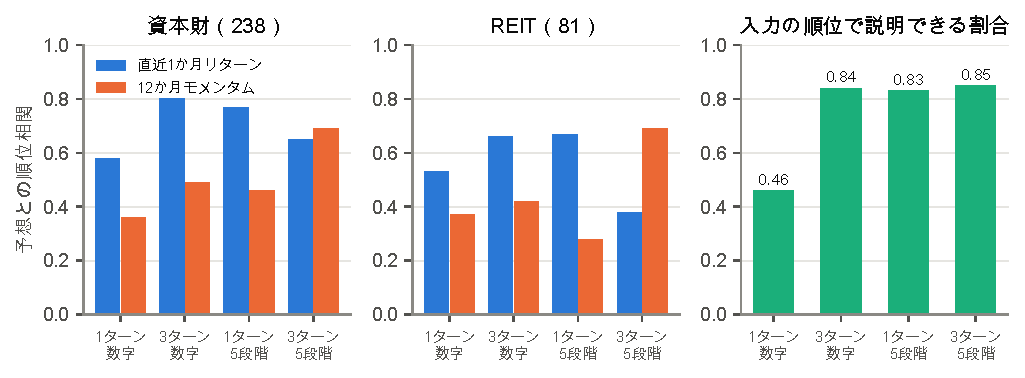
\includegraphics[width=\linewidth]{exp_f.pdf}
\caption{左・中：予想と値動きの指標の順位相関。右：予想の順位を、8 つの入力の順位で回帰したときの決定係数（資本財）。}
\label{fig:expF}
\end{figure}

\begin{table}[htbp]
\centering
\caption{予想の順位を、8 つの入力の順位で回帰した結果（資本財、213 件）。}
\small
\begin{tabular}{lrrrr}
\toprule
 & 1 ターン・数字 & 3 ターン・数字 & 1 ターン・5 段階 & 3 ターン・5 段階 \\
\midrule
決定係数 & 0.46 & 0.84 & 0.83 & 0.85 \\
直近 1 か月のリターンの係数 & 0.60 & 0.79 & 0.75 & 0.60 \\
12 か月のモメンタムの係数 & 0.31 & 0.43 & 0.39 & 0.64 \\
売上高の前年同期比の係数 & 0.12 & 0.07 & 0.13 & 0.09 \\
純利益の前年同期比の係数 & $-0.04$ & 0.05 & 0.11 & 0.10 \\
PER の係数 & 0.01 & $-0.04$ & 0.01 & 0.01 \\
ROE の係数 & 0.28 & 0.05 & 0.15 & 0.11 \\
\bottomrule
\end{tabular}
\end{table}

\begin{itemize}
\item \textbf{3 ターン・数字}：直近 1 か月のリターンとの相関が、資本財で $+0.58$ から $+0.80$ に、REIT で $+0.53$ から $+0.66$ に上がった。
\item \textbf{1 ターン・5 段階}：答えの形を変えただけでも、相関は上がった（資本財で $+0.77$）。
\item \textbf{3 ターン・5 段階}：直近 1 か月のリターンとの相関は、REIT では下がったが（$+0.38$）、資本財では元より高い（$+0.65$）。どちらの業種でも、12 か月のモメンタムとの相関が $+0.69$ に上がった。なぞる対象が移っただけである。
\item 新しい 3 つの条件は、どれも決定係数が 0.83〜0.85 である。予想の順位の 8 割以上が、入力の順位の足し算で説明できる。
\end{itemize}

\section{結果 2：原因は、LLM 自身のターン 1 の回答にある}

ターン 1 の回答 32 個を読むと、型がほぼ同じだった。

\begin{table}[htbp]
\centering
\caption{ターン 1 の回答に含まれていた内容。}
\small
\begin{tabular}{p{8.40cm}rr}
\toprule
回答に含まれていた内容 & REIT（12 業種） & それ以外（20 業種） \\
\midrule
「モメンタムと直近のリターンが短期の予想の鍵」 & \multicolumn{2}{c}{32 業種のうち 30} \\
「PER と PBR は誤解を招く」 & 12 & 9 \\
「純利益率と ROE は誤解を招く」 & 0 & 10 \\
「純利益率と ROE は効率を表す」（肯定） & 12 & 8 \\
業界で使う FFO に触れた & 0 & --- \\
\bottomrule
\end{tabular}
\end{table}

\begin{itemize}
\item 32 業種のうち 30 業種で、LLM は自分から「モメンタムと直近のリターンが短期の予想の鍵」と答えた。会話にすると、自分が書いたこの方針が手元にある状態で数字を答えるので、方針どおりに答える。
\item REIT の 12 業種すべてで「PER は誤解を招く」と答えたこと自体は正しい。しかし、同じ文が人材サービスや電気部品など、REIT 以外の 9 業種にも出てくる。理由は、どれも「会計の慣行が違うため」である。REIT の事情を踏まえた答えとは言い切れない。
\item REIT の純利益が当てにならないことには、たどり着いていない。純利益率と ROE を 12 業種すべてで肯定し、FFO には一度も触れなかった。
\end{itemize}

\section{結果 3：予想の大きさとばらつき}

\begin{table}[htbp]
\centering
\caption{数字で答えさせた条件の、予想の大きさ（資本財）。}
\small
\begin{tabular}{lrr}
\toprule
 & 1 ターン・数字 & 3 ターン・数字 \\
\midrule
予想の平均（日次） & 0.17\% & 0.07\% \\
銘柄の間の予想のばらつき & 0.22\% & 0.14\% \\
30 個の回答のばらつき & 0.20\% & 0.07\% \\
日次 1\% を超える回答の割合 & 2.7\% & 0.4\% \\
\bottomrule
\end{tabular}
\end{table}

桁は壊れていない。しかし、30 個の回答のばらつきが約 3 分の 1 になった。Black-Litterman では回答の分散を「予想の不確かさ」として使うので、分散が小さくなると、予想をさらに強く信じることになる。元の計算の問題（予想を 99.9\% 採用する）を悪化させる向きである。

5 段階の条件では、回答が偏った。「0（同じくらい）」は 8〜9\% しか選ばれず、約半分が「$-1$」だった。「セクターのほかの銘柄と比べて」と聞いているので、本来は上下が同じくらいになるはずである。30 個の回答はほぼ同じ段階に集まり、ばらつきは 5 段階の目盛りで 0.2 程度だった。

\section{結論}

\begin{keybox}
なぞりは、「知識が使われていない」のではなく、「1 か月先は値動きで決まる」というモデルの見方そのものである。会話にすると、その見方が固まる。
\end{keybox}

\begin{itemize}
\item 3 ターンにしても、なぞりは減らず、強まった。
\item 答えを 5 段階にしても、なぞりは減らなかった。「入力の数字と答えの単位が同じだから足してしまう」という説明だけでは足りない。
\item 業種の知識は、型どおりの一言にとどまる。
\item モデルは「短期だから値動きを重視する」と述べている。予想の期間を長くすれば、答えが変わる可能性がある。
\end{itemize}

この実験には、条件の違いが 1 つ混ざっている。3 ターンの条件では、ターン 2 でセクター、市場、レポートの情報も渡した。ただし、同じセクター・同じ月の銘柄には同じ情報なので、銘柄の間の順位相関には直接は効かない。

% ------------------------------------------------------------
\chapter{実験 G：リスクプレミアムの有無を聞く}\label{ch:expG}

\section{問い}

実験 D〜F は、銘柄ごとに数字を渡して予想させる形だった。この形では、予想は銘柄の値動きの順位で決まった。そこで、形を根本から変えた。\textbf{銘柄の数字は一切渡さず、リスクの種類ごとに「翌月、そのリスクを取ることは報われるか」を聞く。}

Black-Litterman の出発点である均衡リターンは、「リスクに見合う上乗せ（リスクプレミアム）」である。LLM の役割を「いまは、どのリスクにプレミアムが付く局面か」の判断に絞れば、銘柄ごとの期待リターンは
\[
\text{均衡リターン} + \sum_{\text{リスクの種類}} \bigl(\text{その銘柄がリスクをどれだけ持つか}\bigr) \times \bigl(\text{LLM が答えたプレミアムの有無}\bigr)
\]
の形で作れる。銘柄がリスクをどれだけ持つか（ベータ、ボラティリティ、PER など）は、統計で計算する。LLM には銘柄の数字を渡さないので、銘柄の値動きの順位を写す道がない。

\section{方法}

\begin{longtable}{p{3.20cm}p{11.20cm}}
\toprule
\textbf{項目} & \textbf{内容} \\
\midrule
\endfirsthead
\bottomrule
\endfoot
判断日 & 30 か月すべて（2024-03-28〜2026-08-31） \\
渡す情報 & 日付、市場の状態（\SP{} の直近 1 か月と 12 か月のリターン、VIX、30 日の実現ボラティリティ、VIX $\div$ 3 か月 VIX、SKEW、短期金利）、判断日までに公表された最新のレポートの要約とリスク \\
問い（リスクの種類） & 7 つ。「高い側のリターンは、低い側より高いか」を聞く（\tabref{tab:gq}） \\
問い（セクター） & 11 個。そのセクターの指標も渡し、「そのセクターのリターンは、\SP{} 全体より高いか」を聞く \\
答えの形 & 1〜5 の数字 1 文字（1 がはっきり低い、3 が同じくらい、5 がはっきり高い） \\
規模 & 30 か月 $\times$ 18 問 $=$ 540 リクエスト。失敗 0 件 \\
\end{longtable}

\begin{table}[htbp]
\centering
\caption{リスクの種類ごとの問い。}
\label{tab:gq}
\small
\begin{tabular}{lll}
\toprule
リスク & 高い側 & 低い側 \\
\midrule
市場 & \SP{} & 3 か月物の国債 \\
ベータ & ベータの高い銘柄 & ベータの低い銘柄 \\
変動の大きさ & 値動きの大きい銘柄 & 値動きの小さい銘柄 \\
割安さ & PER の低い銘柄 & PER の高い銘柄 \\
勢い & 過去 12 か月で最も上がった銘柄 & 最も上がらなかった銘柄 \\
安全性 & 長期負債の軽い会社 & 重い会社 \\
規模 & 指数の中で小さい会社 & 最も大きい会社 \\
\bottomrule
\end{tabular}
\end{table}

\subsection{回答の確率を直接読む}

この実験では、30 個の回答を数える代わりに、API から「各数字を選ぶ確率」を直接受け取った。答えを 1 文字に限り、その 1 文字について、候補ごとの確率を返させる。1〜5 の確率から、点数（確率で重み付けした平均）と、分布の広がりを計算する。比べるために、同じリクエストで 30 個の回答も取った。

\subsection{当たったかどうかの測り方}

銘柄を並べる必要がないので、この実験では「当たったか」まで見られる。翌月に実際に付いたプレミアムを、次のように計算した。

\begin{itemize}
\item リスクの種類：判断日の指標で銘柄を 3 つに分け、高い側の 3 分の 1 と低い側の 3 分の 1 の、翌月のリターン（等金額の平均）の差。
\item 市場：\SP{} の翌月のリターン $-$ 短期金利の 1 か月分。
\item セクター：セクター ETF の翌月のリターン $-$ \SP{} のリターン。
\end{itemize}

\section{結果 1：確率の読み取りは使える。しかし、なめらかではない}

\begin{figure}[htbp]
\centering
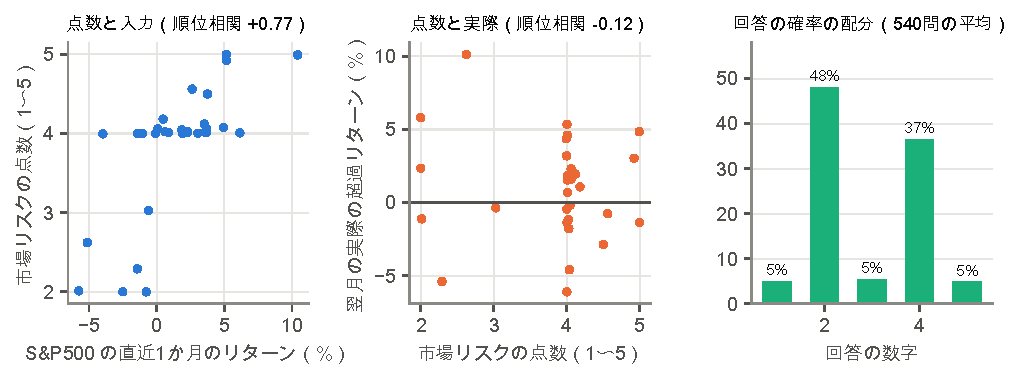
\includegraphics[width=\linewidth]{exp_g.pdf}
\caption{左：市場リスクの点数と、渡した \SP{} の直近 1 か月のリターン。中：点数と、翌月の実際の超過リターン。右：回答の確率の配分。}
\label{fig:expG}
\end{figure}

\begin{itemize}
\item 確率から作った点数と、30 個の回答の平均の相関は 0.997 だった。30 回聞く必要はなく、1 回で済む。
\item しかし、確率は 1 つの数字に集中する（例：「4 が 94\%、5 が 6\%」）。分布の広がりは、1〜5 の目盛りで 0.2〜0.3 しかない。
\item 「3（同じくらい）」は、全体の 5.5\% しか選ばれない。ほぼ「2」か「4」の二択である。
\end{itemize}

LLM なら確信の度合いをなめらかに表せるのではないか、という期待は、gpt-4o-mini については当たらなかった。

\section{結果 2：リスクの種類}

\begin{table}[htbp]
\centering
\caption{リスクの種類ごとの結果（30 か月）。「的中率」は、点数が 3 より上か下かと、実際のプレミアムの符号が合った月の割合。右の 3 列は順位相関で、「点数と直近リターン」は \SP{} の直近 1 か月のリターンとの相関。}
\label{tab:gfactors}
{\small
\resizebox{\linewidth}{!}{%
\begin{tabular}{lrrrrrrr}
\toprule
リスク & 点数の平均 & 点数 $>3$ の月 & 実際 $>0$ の月 & 的中率 & 点数と実際 & 点数と直近リターン & 点数と VIX \\
\midrule
市場 & 3.82 & 25 & 17 & 0.53 & -0.12 & +0.77 & -0.59 \\
ベータ & 4.00 & 26 & 21 & 0.57 & -0.14 & +0.47 & -0.49 \\
変動の大きさ & 3.69 & 25 & 17 & 0.40 & -0.02 & +0.62 & -0.38 \\
割安さ & 3.77 & 26 & 17 & 0.70 & -0.15 & +0.42 & -0.42 \\
勢い & 4.07 & 27 & 16 & 0.43 & +0.06 & +0.58 & -0.51 \\
安全性 & 4.10 & 30 & 17 & 0.57 & -0.11 & +0.45 & -0.36 \\
規模 & 3.30 & 20 & 11 & 0.50 & +0.07 & +0.34 & -0.37 \\
\bottomrule
\end{tabular}}
}
\end{table}

\begin{figure}[htbp]
\centering
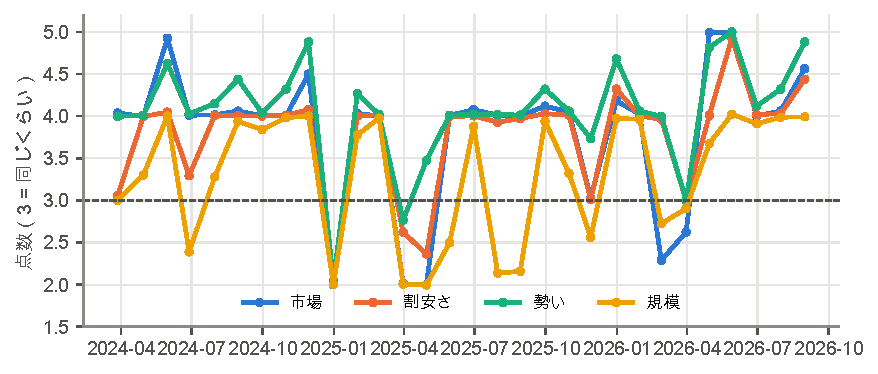
\includegraphics[width=0.95\linewidth]{exp_g_series.pdf}
\caption{4 つのリスクの点数の推移。別々のリスクについて聞いているのに、同じ月に同じ向きに動く。}
\label{fig:expGseries}
\end{figure}

\begin{itemize}
\item \textbf{ほぼ毎月「報われる」と答える。}どのリスクも、30 か月のうち 20〜30 か月で「高い側が勝つ」だった。実際に高い側が勝った月は、11〜21 か月である。
\item \textbf{当たっていない。}点数と実際のプレミアムの順位相関は、$-0.15$ から $+0.07$ である。30 か月では $\pm 0.36$ までは偶然で出るので、「関係が見られない」が正確である。
\item \textbf{7 つの答えが、そろって動く。}\figref{fig:expGseries} のとおりである。割安さと勢いのように、本来は別々に動くはずのものも、同じ向きである。
\item \textbf{点数は、渡した市場の数字に沿っている。}市場リスクの点数は、\SP{} の直近 1 か月のリターンと順位相関が $+0.77$、VIX とは $-0.59$ だった。ほかのリスクでも、向きは同じである。
\end{itemize}

「先月上がって VIX が低ければ、どのリスクも報われる」という、1 つのつまみで全部の答えが決まっている。

\section{結果 3：セクター}

\begin{figure}[htbp]
\centering
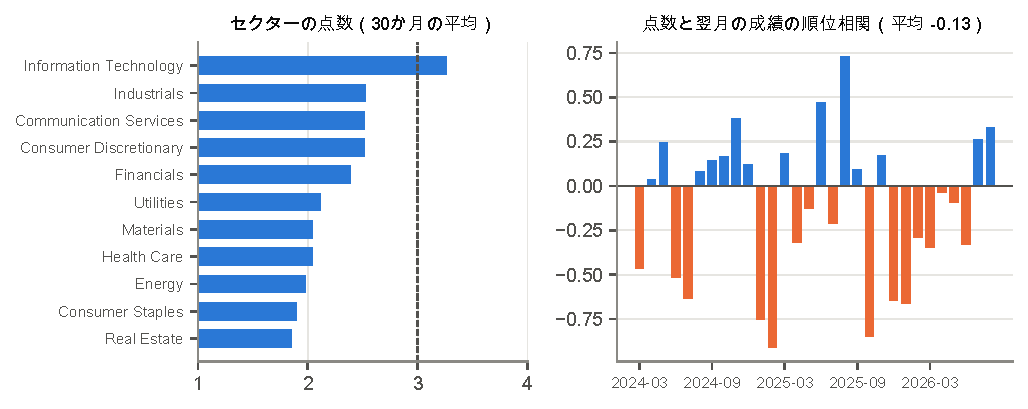
\includegraphics[width=\linewidth]{exp_g_sector.pdf}
\caption{左：セクターごとの点数の平均。3 が「指数と同じくらい」。右：点数と翌月の成績の、月ごとの順位相関。}
\label{fig:expGsector}
\end{figure}

\begin{itemize}
\item \textbf{点数は、セクターのモメンタムに沿っている。}11 セクターの間の順位相関は、3 か月のモメンタムと $+0.72$、12 か月と $+0.75$ だった。渡したセクターの指標をなぞっている。
\item \textbf{翌月の実際の成績とは合わない。}月ごとの順位相関の平均は $-0.13$（$t$ 値 $-1.64$。プラスは 30 か月のうち 14 か月）。点数の上位 3 セクターから下位 3 セクターを引いた成績は、月 $-0.58\%$（$t$ 値 $-0.79$）だった。どちらも偶然の範囲で、「逆に当たる」とまでは言えない。
\item \textbf{答えが偏っている。}72\% が「2（指数よりやや低い）」だった。情報技術（平均 3.26）以外のほぼ全セクターが指数に負ける、という答えで、つじつまが合わない。
\end{itemize}

この期間は、セクターのモメンタムそのものが、翌月の成績とやや逆向きだった（順位相関 $-0.07$〜$-0.20$）。モメンタムに沿って答えたことが、裏目に出た形である。

\section{結論}

\begin{itemize}
\item 回答の確率を直接読む方法は、30 個の回答の平均の代わりに使える。費用は 30 分の 1 で済む。
\item 枠組みをリスクプレミアムに変えても、答えは渡した数字の中の「直近の値動き」に沿った。銘柄の数字を渡さなければ、市場のリターンとセクターのモメンタムに沿う。
\item この実験では、レポートの文章が効いているのかどうかを分けていない。「文章だけを渡す」「数字だけを渡す」の 2 条件を足せば分かる。次に行うべき実験である。
\end{itemize}

% ------------------------------------------------------------
\chapter{実験の総合考察}\label{ch:synthesis}

\section{くり返し現れた 1 つの性質}

4 つの実験（D〜G）は、入力と質問の形をそれぞれ変えている。それでも、同じ結果が形を変えて現れた。

\begin{longtable}{cp{5.20cm}p{8.40cm}}
\toprule
 & \textbf{変えたこと} & \textbf{予想が沿っていたもの} \\
\midrule
\endfirsthead
\bottomrule
\endfoot
既存 & 1 か月分の日次リターンの列を渡す & 渡した月の平均リターン（相関 0.89） \\
D & 日次リターンの列を、要約した指標に置き換える。財務の指標を足す & 直近 1 か月のリターン（順位相関 $+0.5$ 前後）、12 か月のモメンタム \\
E & 考慮する比率を明言する & 直近 1 か月のリターン。値動きを 0\% にすると、成長率 \\
F & 3 ターンの会話にする。答えを 5 段階にする & 直近 1 か月のリターン、または 12 か月のモメンタム（より強く） \\
G & 銘柄の数字を渡さず、リスクの種類ごとに聞く & 市場の直近 1 か月のリターンと VIX。セクターはセクターのモメンタム \\
\end{longtable}

\begin{keybox}[実験から言えること]
gpt-4o-mini は、渡された数字の中から「直近の値動き」に当たるものを見つけ、その向きに答える。上がったものは上がり続け、下がったものは下がり続ける、という答えである。
\end{keybox}

\section{なぜそうなるか}

実験 F のターン 1 の回答が、手がかりになる。LLM は、32 業種のうち 30 業種で、自分から「モメンタムと直近のリターンが短期の予想の鍵」と答えた。つまり、なぞりは不具合ではなく、「1 か月先のリターンは、最近の値動きの延長で決まる」というモデルの見方が、そのまま出たものである。

この見方は、金融の実証研究の知見とは合わない。個別の銘柄の 1 か月のリターンは、続くよりも反転しやすいことが知られている。実際、本プロジェクトのデータでも、予想と翌月の実際のリターンの順位相関は $+0.05$ で、セクターでは負だった。Chen ほか（2024）は、LLM の予想が直近の成績に重みを置きすぎることを報告していて、本プロジェクトの結果と一致する（\chapref{ch:literature}）。

\section{ほかに分かったこと}

\begin{description}[leftmargin=2em,style=nextline,itemsep=0.4em]
\item[「率」の形をした数字だけが使われる] リターンや成長率のように、答えと同じ形の数字は使われる。PER や ROE のような水準の指標は、どの条件でも使われなかった。
\item[業種の知識は、聞けば出るが、浅い] 「REIT の PER は誤解を招く」とは言えるが、同じ文がほかの業種にも出てくる。業界で使う指標（FFO）には触れない。
\item[回答はそろいすぎる] 30 個の回答のばらつきは、予想の当たり具合を表さない。会話にすると、ばらつきはさらに小さくなる。確率を直接読んでも、1 つの答えに集中する。
\item[答えが楽観に偏る] 銘柄の予想は 76\% がプラスで、リスクプレミアムは、ほぼ毎月「付く」と答えた。一方、セクターを指数と比べる問いでは、72\% が「指数より低い」だった。問いの形によって偏りの向きが変わり、全体としてつじつまが合わない。
\item[数字を足し算に使う] 重みを指定すると、渡した数字をそのまま重み付きで足す。
\end{description}

\section{設計への示唆}

これらの結果は、「LLM に数字を読ませて、銘柄の順位を付けさせる」方向の限界を示している。数字の読み方について、gpt-4o-mini は統計モデルと同じか、それより単純なことしかしていない。

考えられる方向は 4 つある。

\begin{longtable}{p{3.80cm}p{5.20cm}p{5.40cm}}
\toprule
\textbf{方向} & \textbf{内容} & \textbf{実験との関係} \\
\midrule
\endfirsthead
\bottomrule
\endfoot
LLM の役割を文章に絞る & 数字は統計モデルに任せ、LLM には文章の解釈だけをさせる & 先行研究で成果が出ている形。まだ確かめていない \\
予想の期間を長くする & 翌月ではなく、四半期や半年先を聞く & モデルは「短期だから値動きを重視する」と述べている \\
値動きを入力から外す & なぞる対象をなくす & 実験 E では、成長率をなぞるようになった \\
読み方をこちらで与える & 業種ごとの指標の読み方を、LLM に答えさせず、人が書いて渡す & LLM 自身の回答は型どおりで、値動き重視に誘導する \\
\end{longtable}

最初に確かめるべきは、「文章だけを渡したとき、LLM の答えは月によって変わるか。その変化は数字に沿っていないか」である。これが成り立たなければ、月次レポートを読ませるという提案手法の中心が成り立たない。実験 G に 2 条件を足すだけで確かめられる（各 540 リクエスト）。

% ============================================================
\part{調査}
% ============================================================

\chapter{先行研究}\label{ch:literature}

実験の結果を受けて、2026 年 10 月 13 日に先行研究を調べた。読んだのは、対象論文の第 2 版（本文）を除き、要旨と要約が中心である。数字を引用するときは、原文で確かめる必要がある。調べたのは検索 6 回分で、網羅はしていない。

\section{LLM の予想は直近の値動きを外挿する}

\textbf{Chen、Green、Gulen、Zhou（2024）「What Does ChatGPT Make of Historical Stock Returns? Extrapolation and Miscalibration in LLM Stock Return Forecasts」}は、本プロジェクトの実験で見つけた性質を、すでに報告している。

\begin{itemize}
\item 実際の株価は短期では反転しやすいのに、LLM の予想は直近の成績に重みを置きすぎる（過剰な外挿）。人間の投資家と同じ偏りである。
\item 予想は、過去と将来の実際のリターンに比べて楽観的である。
\item 80\% の信頼区間を聞くと、人間のアンケートよりは幅が妥当だった。ただし、極端な値については悲観的で、分布が偏る。
\end{itemize}

本プロジェクトの結果（予想と直近 1 か月のリターンの順位相関が $+0.5$〜$0.8$、予想の 76\% がプラス）と、そのまま重なる。本プロジェクトは、この既知の偏りが Black-Litterman の入力の段階でどう効くか（予想が 99.9\% 採用され、比率が数銘柄に集中する）を確かめたもの、と位置づけられる。

\section{数字を渡しても良くならない}

\begin{itemize}
\item \textbf{「Predictive Power of LLMs in Financial Markets」（arXiv:2411.16569）}は、プロンプトに特定の数値データを足しても、予測が良くなるとは限らないと報告している。
\item \textbf{Tan ほか（NeurIPS 2024）「Are Language Models Actually Useful for Time Series Forecasting?」}は、時系列の予測に LLM を使う手法から LLM を外しても、精度が下がらないことを示した。著者らは、時系列の「予測」ではなく、「推論」や金融の判断のほうに可能性があると述べている。
\end{itemize}

\section{文章を読ませると効く}

\begin{longtable}{p{4.60cm}p{3.40cm}p{6.40cm}}
\toprule
\textbf{論文} & \textbf{LLM に渡すもの} & \textbf{結果} \\
\midrule
\endfirsthead
\toprule
\textbf{論文} & \textbf{LLM に渡すもの} & \textbf{結果} \\
\midrule
\endhead
\bottomrule
\endfoot
Lopez-Lira と Tang「Can ChatGPT Forecast Stock Price Movements?」 & ニュースの見出し & 見出しの良し悪しの採点が、その後のリターンと関係した。ただし、LLM が普及するにつれて効果は薄れている \\
Anic、Barbon、Seiz、Zarattini（2025）「ChatGPT in Systematic Investing」 & 銘柄ごとのニュース & モメンタムで選んだ銘柄について「ニュースがその流れを支持するか」を判定させ、採否と比率に反映した。ふつうのモメンタム戦略を上回った \\
Lehner と Lopez-Lira（2026）「ChatGPT as a Time Capsule」 & なし（モデルの知識そのもの） & 知識の期限が違う 12 個のモデルから銘柄の見通しの点数を作り、1 か月先のリターンと関係した \\
Kim、Muhn、Nikolaev（2024）「Financial Statement Analysis with Large Language Models」 & 匿名にした財務諸表 & 手順を踏んで考えさせると、利益の増減の方向を約 60\% 当てた。アナリストを上回り、専用の機械学習モデルと同じ程度 \\
\end{longtable}

Anic ほかの形は、本プロジェクトの実験の結論と同じ方向である。数字（モメンタム）は統計で扱い、LLM には文章の判断だけをさせている。

Kim ほかは、本プロジェクトの結果（財務の数字が使われない）と逆に見える。ただし、違いが 3 つある。予測するのがリターンではなく利益の方向であること、モデルが GPT-4 であること、数字を返す前に比率の計算と解釈を書かせていることである。

\section{未来の情報の混入}

\begin{itemize}
\item \textbf{「The Memorization Problem」（arXiv:2504.14765）}は、GPT-4o が知識の期限（2023 年 10 月）より前の \SP{} の水準を思い出せること、期限の後は思い出せないことを報告している。「過去の時点のつもりで答えて」と指示しても、防げない。
\item 対策として、知識の期限を固定したモデルを作る研究（DatedGPT、arXiv:2603.11838）や、評価の枠組み（Look-Ahead-Bench、arXiv:2601.13770）が 2026 年に出ている。
\end{itemize}

「知識が 2023 年 10 月までの gpt-4o-mini を使い、評価は 2024 年 4 月から」という本プロジェクトの設計は、この問題への正しい対処だと確かめられた。

\section{対象論文の第 2 版}

対象論文には、2025 年 10 月に第 2 版が出ている。内容は \secref{sec:v2} にまとめた。本プロジェクトにとって大事な点は 3 つある。

\begin{itemize}
\item 第 2 版自身が、gpt-4o-mini を使った Black-Litterman の成績（年率 $+7.7\%$）が等金額（$+19.1\%$）を下回ることを報告している。
\item 第 2 版は、予想が入力の何に沿っているかを分析していない。本プロジェクトの実験は、その空白を扱っている。
\item 対象の銘柄を、評価期間の途中の時価総額で選んでいる。
\end{itemize}

\section{本プロジェクトの位置づけ}

\begin{figure}[htbp]
\centering
\begin{tikzpicture}[x=10mm,y=10mm]
\node[box=c3,minimum width=38mm,minimum height=13mm] (a) at (0,0) {Chen ほか（2024）\\{\scriptsize LLM の予想は外挿する}};
\node[box=c1,minimum width=42mm,minimum height=13mm] (b) at (4.7,0) {\textbf{本プロジェクト}\\{\scriptsize その予想を BL に入れると、どうなるか}};
\node[box=c3,minimum width=38mm,minimum height=13mm] (c) at (9.4,0) {Lee ほか（2025）\\{\scriptsize LLM の予想を BL に入れる}};
\node[box=c4,minimum width=42mm,minimum height=13mm] (d) at (4.7,-2.0) {Anic ほか（2025）\\{\scriptsize 数字は統計、文章は LLM}};
\draw[arr] (a) -- (b);
\draw[arr] (c) -- (b);
\draw[arr,dashed] (b) -- node[lab,right]{次に確かめる方向} (d);
\end{tikzpicture}
\caption{先行研究との関係。}
\end{figure}

見つけた範囲では、運用会社の月次レポートを LLM に読ませて Black-Litterman の入力にする例はなかった。ただし、効果が報告されているのは銘柄ごとのニュースである。月次レポートは全銘柄で同じ文章なので、銘柄の差を作れない。過去のニュースの見出しが手に入るかは、調べる価値がある。

% ------------------------------------------------------------
\chapter{そのほかの調査と検討}\label{ch:other}

作業の途中で調べたこと、相談して決めたことを、項目ごとにまとめる。

\section{モデルの選択と費用}

\begin{itemize}
\item 全銘柄・30 か月の予想（約 1.5 万リクエスト、各 30 個の回答）は、gpt-4o-mini で約 1.75 ドルだった。
\item OpenAI の API は、1 回のリクエストで複数の回答を返す設定（\code{n}）を持つ。入力を 1 回送るだけで 30 個の回答を受け取れるので、時間と費用が大きく下がる。
\item Anthropic の Claude の API には、この設定がない。同じ質問を 30 回送る必要があり、当時の試算では約 50 倍の費用になった。
\item より新しいモデルは、評価期間（2024 年 4 月以降）の相場を学習で知っている可能性がある。モデルを比べるなら、成績を知識の期限の前と後で分けて出す必要がある。
\item 予算の上限は、全部合わせて 5 万円（300 ドル強）としている。
\end{itemize}

以上から、gpt-4o-mini を使い続け、モデルの比較は論点の中心にしないと決めた。

\section{オプション市場の情報}

霧生・枇々木（2014）「複数資産にインプライド分布を用いた最適資産配分モデル」（日本オペレーションズ・リサーチ学会和文論文誌）を参考にした。この論文は、資産の将来のリターンの分布を、過去のデータではなく、オプションの価格から逆算した分布（インプライド分布）から作る。国内外の株式と債券の 4 資産で、過去データだけの場合より成績が良いことを示している。

本プロジェクトで使える考え方は、次の点である。

\begin{itemize}
\item オプションの価格は、判断日の時点の「将来の見通し」である。判断日の市場の価格そのものなので、未来の情報が混ざる心配がない。
\item 過去データから見積もった平均は成績を下げる、という結果は、期待リターンを過去の平均から取らず、市場の均衡と予想から作る方針の裏づけになる。
\end{itemize}

実際に使えるデータを調べると、個別の銘柄やセクターのオプションの過去の価格は、無料では手に入らなかった（\chapref{ch:sector}）。市場全体については、VIX などの指数が全期間取れる。VIX は \SP{} のオプションから計算された指数なので、オプションの情報の要約として使える。

なお、株価指数の先物からは、期待リターンは取れない。先物の価格は「現物 $+$ 持ち越しのコスト」で決まり、相場の見通しは入っていない。オプションから出る分布も、中心は無リスク金利に固定される。

\section{統計モデルでビューを作れるなら、LLM は要るか}

「ロジスティック回帰の結果からビューを作れるなら、LLM を回す必要はあるか」という問いを検討した。

\begin{itemize}
\item Black-Litterman のビューは、もともと人間のアナリストの見通しである。統計モデルから作ることも、ふつうに行われる。回帰が出す「上がる確率」は、式~\eqref{eq:grinold} のような形で期待リターンに直せる。
\item したがって、数字だけを使うなら、LLM は要らない。LLM を使う意味があるとすれば、回帰では扱えない文章を読めることである。
\item この問いは、実験の結果によって、さらに重くなった。数字の読み方では、gpt-4o-mini は統計モデルを上回る働きをしていない。
\end{itemize}

\section{セクターの情報源}

\begin{itemize}
\item セクター別の ETF は、値動きの情報源として使える（\chapref{ch:sector}）。ただし、ETF の値動きをそのまま LLM に渡すと、既存手法と同じ「なぞり」が起きる。実験 G で、実際にそうなった。
\item 運用会社のセクター・スコアカード（ステート・ストリート）は、内容は理想的だが、7 か月分しか手に入らなかった。公表も翌月の 10 日ごろで、判断日には間に合わない。自作の指標の答え合わせにだけ使った。
\item セクターごとの見通しを文章で書いた資料を、30 か月分そろえる方法は、まだ見つかっていない。
\end{itemize}

\section{予想をリターンに直す方法}

実験 F と G を踏まえて、答えの形を検討した。

\begin{itemize}
\item 「かなり上がりそう」から「かなり下がりそう」までの 5 段階に分け、段階ごとに係数を掛ける方法は、採らない。係数に根拠がない。
\item 連続の値を取る方法は 3 つある。0〜100 の点数で答えさせる、回答の確率を API から直接読む、多数の回答を平均する。2 つ目は実験 G で試し、30 個の平均と同じ値が得られた。ただし、gpt-4o-mini の確率は 1 つの答えに集中する。
\item 点数をリターンに直すには、式~\eqref{eq:grinold} を使う。決める係数は「当たり具合（IC）」の 1 つで、過去のデータから測れる。予想の大きさが現実的になるので、比率の集中の問題も和らぐ。
\end{itemize}

\section{Black-Litterman の動きについての確認}

「前月の比率から逆算して、新しいビューで更新しているのか」という問いを確かめた。答えは「いいえ」である。逆算の出発点は、判断日その日の市場の時価総額の比率で、毎月ゼロから計算し直す。前月の更新の結果も、前月に決めた比率も、引き継がない。前月の比率が関わるのは、売買の量（回転率）だけである。

公式実装は、そもそも逆算を使っていない。事前の期待リターンを「ベータ $\times$ 市場の平均超過リターン」で出している（\secref{sec:original-calc}）。

% ============================================================
\part{まとめ}
% ============================================================

\chapter{評価の観点から見た現状}\label{ch:eval}

授業の採点の基準は分からないので、研究の課題で一般に見られる 8 つの観点で、現状を整理する。

\begin{longtable}{p{3.40cm}p{6.00cm}p{5.00cm}}
\toprule
\textbf{観点} & \textbf{示せること} & \textbf{根拠} \\
\midrule
\endfirsthead
\toprule
\textbf{観点} & \textbf{示せること} & \textbf{根拠} \\
\midrule
\endhead
\bottomrule
\endfoot
1. 批判的に読めているか & 元の実装の 9 つの問題点を、数字で確かめた。元の設定のままの結果と、直した結果の両方を残した & \chapref{ch:problems}、\chapref{ch:blm} \\
2. 設計が妥当か & 未来の情報が混ざる経路を 6 つ挙げ、5 つをふさいだ。AI に書かせたレポートに後の情報が混ざる実例を示した & \chapref{ch:policy} \\
3. データの扱いが丁寧か & 出どころと取得日が明確。実際の指数と照合した（相関 0.9997）。除外した銘柄を明示した。財務データを別の出どころと照合した（97.6\% が一致） & \chapref{ch:data} \\
4. 比較が公平か & 全戦略に同じ銘柄、同じ期間、同じ除外を適用した。配当の扱いをそろえた & \chapref{ch:blm} \\
5. 結果を説明できるか & 元の成績が良く見える理由を、4 つの問題のつながりで説明した。予想が何に沿っているかを、7 つの実験で確かめた & \chapref{ch:problems}、第 V 部 \\
6. 再現できるか & 実行ごとに条件と全回答を保存している。設定は 1 か所にある。実験のスクリプトと全回答を残している & \chapref{ch:system}、付録 \\
7. 限界を述べているか & 評価期間の短さ、生存者バイアス、近似の構成比率、実験の規模の小ささを明記した & \secref{sec:limits} \\
8. 独自の拡張があるか & 月次レポートの読み取り、セクターと銘柄の指標、質問の形を変える実験、確率の直接の読み取り & 第 IV 部、第 V 部 \\
\end{longtable}

\section{評価を下げかねない点と備え}

\begin{longtable}{p{4.20cm}p{5.00cm}p{5.20cm}}
\toprule
\textbf{点} & \textbf{内容} & \textbf{備え} \\
\midrule
\endfirsthead
\bottomrule
\endfoot
結果が良すぎる & 指数を大きく上回る成績は、まず先読みか計算の誤りを疑われる & 元の計算の年率 $+35\%$ は、成果として示さない。理由を説明する対象として示す \\
「勝った」ことを結論にする & 30 か月では、統計的に強いことは言えない & 結論は「この設計で、こう検証した結果、こうだった」にする \\
提案手法の成果がまだない & 改善した手法の成績は出ていない & 「なぜ既存手法が働いていないか」と「どの改善が効かないか」を、数字で示している \\
作ったものが多く、筋が見えにくい & データ基盤、指標、レポート、実験が並ぶ & 主張を 1 つに決める（次の節） \\
元の研究と直接比べられない & モデル、期間、銘柄が違う & 違いを表にまとめ、「公式実装の計算」を確かめたものだと明記する \\
\end{longtable}

\section{主張の軸}

これまでの結果から、主張の軸は次のように置ける。

\begin{keybox}[主張]
LLM に数値のデータを渡して将来のリターンを予想させると、LLM は直近の値動きを外挿する。その予想を Black-Litterman モデルに入れると、回答のばらつきが小さいために予想がほぼそのまま採用され、モデルの本来の働き（市場の比率を出発点にして少し動かす）が失われる。この性質は、入力の内容や質問の形を変えても残る。LLM を使うなら、数値の処理ではなく、文章の解釈に役割を絞るべきである。
\end{keybox}

当初は「未来の情報が混ざる経路をふさいだ設計」を見せ場にする計画だった。この設計は土台として残る。その上で、実験から得た「LLM は何を足していて、何を足していないか」という問いへの答えが、より強い主張になった。

% ------------------------------------------------------------
\chapter{課題と今後の計画}\label{ch:future}

\section{限界}\label{sec:limits}

\begin{longtable}{p{4.20cm}p{10.20cm}}
\toprule
\textbf{限界} & \textbf{結論への影響} \\
\midrule
\endfirsthead
\toprule
\textbf{限界} & \textbf{結論への影響} \\
\midrule
\endhead
\bottomrule
\endfoot
評価は 30 か月分だけ & 成績の差が出ても、偶然と区別できない場合が多い。順位相関は、30 か月では $\pm 0.36$ までは偶然で出る \\
相場の局面が偏っている & 期間全体で指数が大きく上がっている。下落相場での挙動は分からない \\
除外した 28 銘柄 & 破綻・買収された銘柄が入っていない。戦略どうしの比較は公平だが、成績の水準には生存者バイアスがある \\
構成比率は近似 & 浮動株で調整していない。年 1\% 未満の差は、近似による差と区別できない \\
社名・セクターは現在のもの & 当時の名称・分類と違う場合がある \\
売買のコストを入れていない & 毎月比率を変える戦略は、実際にはコストの分だけ成績が下がる \\
モデルは 1 つだけ & 結果が gpt-4o-mini に固有のものかどうかは分からない。先行研究（Chen ほか）は、別のモデルで同じ性質を報告している \\
実験の規模が小さい & 実験 D は 5 つ、E と F は 3 つの判断日だけ。傾向は一貫しているが、数値の細かい大小は当てにならない \\
実験の条件が完全にはそろっていない & 実験 F の比較の相手（1 ターン・数字）は、予想の指示の置き場所が少し違う。3 ターンの条件は、入力も増えている \\
財務データの欠け & 2026 年 4〜6 月期が 57 銘柄で欠けている。負債の指標は、約半分の銘柄にしかない \\
\end{longtable}

\section{決めていないこと}

\begin{longtable}{p{4.60cm}p{5.00cm}p{4.80cm}}
\toprule
\textbf{決めること} & \textbf{選択肢} & \textbf{今の考え} \\
\midrule
\endfirsthead
\toprule
\textbf{決めること} & \textbf{選択肢} & \textbf{今の考え} \\
\midrule
\endhead
\bottomrule
\endfoot
比率の集中への対処 & 指数からのずれに上限 ／ 予想を当たり具合で縮める ／ 銘柄ごとの上限 & 上限を付ける案と、式~\eqref{eq:grinold} で縮める案を、成績を見ずに決める \\
設定を選ぶ期間と、成績を示す期間の区切り & 前半と後半に分ける & 前半で選び、後半で示す。区切りは結果を見る前に決める \\
LLM の役割 & 銘柄ごとの予想 ／ リスクの種類ごとの判断 ／ 文章の解釈だけ & 文章の解釈に絞る方向。次の実験で確かめる \\
予想の期間 & 1 か月 ／ 四半期 & 四半期を試す。モデルの答えが変わるかを見る \\
上場直後の銘柄 & 入力の日数に下限を設ける & 下限を設けて外す \\
自社株買いで純資産が小さい会社 & ROE と PBR を作らない決まりを足す & 未決定 \\
発行済み株式数のならし & 前後の報告の中央値でならす & 未決定 \\
\end{longtable}

\section{次に行うこと}

優先の高い順に並べる。

\begin{enumerate}
\item \textbf{文章だけを渡す実験}：実験 G に「文章だけを渡す」「数字だけを渡す」の 2 条件を足す。LLM が文章から独自の判断を出せるかを確かめる。各 540 リクエストで、数分で終わる。
\item \textbf{予想の期間を延ばす実験}：実験 F のターン 1 の質問で、「翌月」を「次の四半期」に変える。モデルが挙げる指標が変わるかを見る。
\item \textbf{比率の集中への対処}：指数からのずれの上限を最適化に足す。予想を式~\eqref{eq:grinold} で縮める形も実装する。
\item \textbf{統計モデルの比べる相手を作る}：\code{stock\_metrics} の指標で、翌月に指数を上回るかを予測するロジスティック回帰を作る。評価期間より前のデータで変数を選ぶ。
\item \textbf{銘柄ごとの文章の情報源を探す}：過去のニュースの見出しや、決算の説明の文章が、公表日つきで手に入るかを調べる。
\item \textbf{プロンプトの組み立てをリポジトリに入れる}：入力のまとまりを選んで並べる処理を \code{llm/} に実装し、実行の記録に「使ったまとまり」を残す。
\item \textbf{結果へのフィードバック}：数字での要因の分解を先に作り、その後で、レポートを参照して説明する LLM を足す。
\end{enumerate}

1 と 2 は、設計の方向を決めるための実験である。3 と 4 は、どの方向に進んでも必要になる。

\section{データと実装の残り}

\begin{itemize}
\item 月次レポートの表の数字を、LLM ではなく PDF の文字から取り出す処理に置き換える。
\item 月次レポートの公表日と実際の公開日のずれを、数本で確かめる。
\item 財務データの欠けている四半期を取り直す。長期負債の項目名の候補を増やす。配当込みの指数を足す。
\end{itemize}

% ------------------------------------------------------------
\chapter{結論}\label{ch:conclusion}

本書は、LLM の予想を Black-Litterman モデルに入れる手法について、再現、検証、拡張の設計、実験を行った 5 日間の記録である。

\textbf{再現について。}公式実装を OpenAI の API で動く形に作り直し、\SP{} の各時点の構成銘柄すべてについて、30 か月分の予想を集めた。データは、無料で取れるものだけで、実際の指数と日次リターンの相関が 0.9997 になる精度で作れた。

\textbf{検証について。}元の計算は、3 つの点で、名前のとおりには働いていなかった。第 1 に、Black-Litterman は LLM の予想をほぼそのまま（99.9\%）採用していて、市場の均衡は使われていない。第 2 に、LLM の予想は渡した月の値動きの写しで（相関 0.89）、翌月の実際のリターンとはほとんど関係がない（順位相関 $+0.05$）。第 3 に、最適化は最適な答えに届く前に止まっていて、比率が十数銘柄に分かれているのはそのためである。計算を正しくすると、比率は 1〜2 銘柄に集中する。元の成績は、「直近 1 か月に値動きの大きかった銘柄に集中した場合の成績」として読むべきである。

\textbf{拡張について。}未来の情報が混ざる経路を整理し、月次レポートの読み取り、セクターの指標、銘柄の指標を実装した。自作の指標は、運用会社の公表値とよく一致した。一方で、LLM にレポートの表の数字を読ませると、1〜2 割の誤りが残った。

\textbf{実験について。}入力を要約に変える、財務の指標を足す、考慮する比率を明言する、会話にする、答えの形を変える、銘柄の数字を渡さない、のどれを試しても、gpt-4o-mini の答えは、渡された数字の中の直近の値動きに沿った。会話にして先に方針を述べさせると、モデルは自分から「1 か月先は値動きで決まる」と答え、なぞりはかえって強まった。これは、先行研究が報告している LLM の過剰な外挿と一致する。

以上から、次のように結論する。\textbf{数値のデータから銘柄のリターンを予想させる使い方では、gpt-4o-mini は統計モデルを上回る働きをしておらず、その予想を回答のばらつきで重み付けして Black-Litterman モデルに入れる方法は、モデルの本来の働きを失わせる。}LLM を使う意味があるとすれば、数値ではなく文章を読む部分である。それが実際に成り立つかどうかは、まだ確かめていない。次に行うべきは、文章だけを渡したときの LLM の判断を調べる実験である。

勝ち負けを示す結果は、まだ何も得られていない。得られたのは、「何が働いていないか」と「なぜ働いていないか」についての、数字による説明である。これが、次の半年の設計の出発点になる。

% ============================================================
\appendix
\part{付録}
% ============================================================

\chapter{用語集}\label{app:glossary}

\begin{longtable}{p{4.20cm}p{10.20cm}}
\toprule
\textbf{用語} & \textbf{意味} \\
\midrule
\endfirsthead
\toprule
\textbf{用語} & \textbf{意味} \\
\midrule
\endhead
\bottomrule
\endfoot
\SP{} & 米国の代表的な株価指数。約 500 社の株式を、時価総額の大きさに応じた比率で組み入れている \\
時価総額 & 株価 $\times$ 発行済み株式数。会社の規模を表す \\
時価総額加重 & 各銘柄を、時価総額に比例した比率で持つこと。\SP{} の比率に近い \\
等金額 & 全銘柄を同じ比率で持つこと \\
平均分散最適化 & 期待リターンと共分散から、リスクに対するリターンが最も良い比率を求める方法 \\
共分散 & 2 つの銘柄の値動きが、どれだけ一緒に動くかを表す量 \\
縮小推定 & データが少ないときに、共分散の推定を単純な形に寄せて安定させる方法 \\
Black-Litterman モデル & 市場の均衡リターンを出発点にし、投資家の見通しを自信の度合いに応じて混ぜる方法 \\
均衡リターン（$\Pi$） & 市場の時価総額の比率が最適になるような期待リターン \\
逆最適化 & 比率から、それが最適になる期待リターンを逆算すること \\
ビュー（$Q$） & 投資家が持つ、将来のリターンについての見通し \\
予想の不確かさ（$\Omega$） & ビューがどれだけ当てにならないかを表す分散 \\
$\tau$ & 均衡リターンの不確かさの大きさを決める係数 \\
リスク回避度（$\delta$） & リスクをどれだけ嫌うかを表す係数 \\
判断日 & 投資比率を決める日。本書では各月の最後の取引日 \\
先読み & 判断した時点では知り得なかった情報を、その判断に使ってしまうこと \\
生存者バイアス & 途中で消えた銘柄（破綻、買収など）が抜けることで、成績が良く見える偏り \\
外挿 & 最近の傾向が、そのまま続くと考えること \\
なぞり & LLM の予想が、渡した数字（とくに直近の値動き）と同じ向き・同じ順位になること。本書での呼び名 \\
モメンタム & 過去の一定の期間のリターン。株価の勢い \\
ボラティリティ & リターンの標準偏差。値動きの大きさ \\
実現ボラティリティ & 過去の実際の値動きから計算したボラティリティ \\
予想ボラティリティ & オプションの価格から逆算した、将来のボラティリティの見通し \\
VIX & \SP{} のオプションから計算される、今後 30 日の予想ボラティリティの指数 \\
ベータ & 市場全体が 1\% 動いたとき、その銘柄が平均して何 \% 動くかを表す数 \\
リスクプレミアム & リスクを取ることへの見返りとして期待される、リターンの上乗せ \\
PER & 株価収益率。時価総額 $\div$ 純利益 \\
PBR & 株価純資産倍率。時価総額 $\div$ 純資産 \\
PSR & 株価売上高倍率。時価総額 $\div$ 売上高 \\
ROE & 自己資本利益率。純利益 $\div$ 純資産 \\
REIT & 不動産投資信託。不動産の賃料などを収益にする会社 \\
FFO & REIT の業界で使う利益の指標。純利益に、減価償却費を足し戻し、物件の売却益を除いたもの \\
GICS & 株式の業種の分類。11 のセクターと、その下のサブ業種からなる \\
ETF & 上場投資信託。指数に連動するように作られ、株式と同じように売買できる \\
EDGAR & 米国証券取引委員会の、企業の開示書類のデータベース \\
シャープレシオ & リスク 1 単位あたりの超過リターン \\
最大下落率 & 資産の最高値からの下落率の最大 \\
回転率 & 1 回の見直しで、比率のうち入れ替わる割合 \\
実質的な銘柄数 & $1/\sum_i w_i^2$。比率の集中の度合い \\
順位相関 & 2 つの量の順位がどれだけそろうかを表す数 \\
情報係数（IC） & 予想と実際のリターンの相関 \\
z スコア & ある値が、集団の平均から標準偏差の何倍離れているか \\
百分位 & 集団の中での位置。0 が最小、100 が最大 \\
temperature & LLM の回答の乱数の強さ。0 にすると、ほぼ同じ答えが返る \\
構造化出力 & LLM の回答を、決まった JSON の形に固定する API の機能 \\
トークン & LLM が文章を処理する単位。費用はトークンの数で決まる \\
\end{longtable}

% ------------------------------------------------------------
\chapter{設定の一覧}\label{app:env}

\code{.env} ファイルの設定の一覧である。値は、リポジトリに入っている \code{.env.example} のもので、実際の実行に使った値とは違うものがある（たとえば、全期間の実行では \code{START\_MONTH} を \code{2024-03-01}、\code{END\_MONTH} を \code{2026-08-01}、\code{TICKERS} を \code{ALL} にした）。

{\footnotesize
\begin{longtable}{p{4.60cm}p{3.60cm}p{6.20cm}}
\toprule
\textbf{設定名} & \textbf{例（.env.example の値）} & \textbf{意味} \\
\midrule
\endfirsthead
\toprule
\textbf{設定名} & \textbf{例（.env.example の値）} & \textbf{意味} \\
\midrule
\endhead
\bottomrule
\endfoot
\texttt{OPENAI\_\allowbreak{}API\_\allowbreak{}KEY} & （各自の API キー。Git には入れない） & .env.example をコピーして .env を作り、OPENAI\_API\_KEY を入れてください \\
\texttt{OPENAI\_\allowbreak{}MODEL} & \texttt{gpt-4o-mini} &  \\
\texttt{SP500\_\allowbreak{}URL} & \texttt{https://\allowbreak{}en.\allowbreak{}wikipedia.\allowbreak{}org/\allowbreak{}wiki/\allowbreak{}List\_\allowbreak{}of\_\allowbreak{}S\%26P\_\allowbreak{}500\_\allowbreak{}companies} & S\&P500 銘柄一覧の取得元と、取得時の User-Agent（Wikipedia は User-Agent がないと 403 を返す） \\
\texttt{SP500\_\allowbreak{}HISTORY\_\allowbreak{}URL} & \texttt{https://\allowbreak{}en.\allowbreak{}wikipedia.\allowbreak{}org/\allowbreak{}wiki/\allowbreak{}Historical\_\allowbreak{}components\_\allowbreak{}of\_\allowbreak{}the\_\allowbreak{}S\%26P\_\allowbreak{}500} & S\&P500 の銘柄入れ替え履歴 \\
\texttt{WIKIPEDIA\_\allowbreak{}API\_\allowbreak{}URL} & \texttt{https://\allowbreak{}en.\allowbreak{}wikipedia.\allowbreak{}org/\allowbreak{}w/\allowbreak{}api.\allowbreak{}php} & 過去の時点の銘柄一覧を読むための Wikipedia の API と、過去の版の URL（\{revid\} は版の番号に置き換わる） \\
\texttt{WIKIPEDIA\_\allowbreak{}REVISION\_\allowbreak{}URL} & \texttt{https://\allowbreak{}en.\allowbreak{}wikipedia.\allowbreak{}org/\allowbreak{}w/\allowbreak{}index.\allowbreak{}php?\allowbreak{}oldid=\allowbreak{}\{revid\}} &  \\
\texttt{USER\_\allowbreak{}AGENT} & \texttt{Mozilla/\allowbreak{}5.\allowbreak{}0 (LLM-BLM research script)} &  \\
\texttt{START\_\allowbreak{}MONTH} & \texttt{2024-06-01} & LLM に渡す月（各月の1日、YYYY-MM-01）。予想するのはその翌月。論文の本番は 2024-06-01 〜 2024-12-01 \\
\texttt{END\_\allowbreak{}MONTH} & \texttt{2024-07-01} &  \\
\texttt{TICKERS} & \texttt{AAPL,NVDA,JPM,XOM,JNJ} & 銘柄（カンマ区切り）。S\&P500 全銘柄なら ALL \\
\texttt{N\_\allowbreak{}SAMPLES} & \texttt{30} & 1銘柄あたりの回答の数（論文は 30）。1回のリクエストでまとめて受け取る \\
\texttt{TEMPERATURE} & \texttt{1.0} & 回答のばらつきの大きさ（OpenAI の標準は 1.0。0 にすると全部同じ答えになる） \\
\texttt{MAX\_\allowbreak{}WORKERS} & \texttt{8} & 同時に聞く銘柄の数 \\
\texttt{RUN\_\allowbreak{}ID} & （空） & 空なら新しい実行として始める。番号を入れると、その実行の続きから再開する（回答済みの銘柄は飛ばす） \\
\texttt{RUN\_\allowbreak{}NOTE} & （空） & 新しい実行に付けるメモ（何を変えた実行か） \\
\texttt{DB\_\allowbreak{}PATH} & \texttt{data/blm.sqlite} & SQLite の DB ファイル（株価・銘柄・LLMの回答を保存） \\
\texttt{DB\_\allowbreak{}START\_\allowbreak{}DATE} & \texttt{2023-03-01} & DB に入れる期間（marketdb/build\_db.py） \\
\texttt{DB\_\allowbreak{}END\_\allowbreak{}DATE} & \texttt{2026-09-30} &  \\
\texttt{ETF\_\allowbreak{}START\_\allowbreak{}DATE} & \texttt{2023-01-01} & セクターETFの株価の開始日（12か月のモメンタムに13か月分が要るので DB\_START\_DATE より前） \\
\texttt{EDGAR\_\allowbreak{}FACTS\_\allowbreak{}URL} & \texttt{https://\allowbreak{}data.\allowbreak{}sec.\allowbreak{}gov/\allowbreak{}api/\allowbreak{}xbrl/\allowbreak{}companyfacts/\allowbreak{}CIK\{cik\}.\allowbreak{}json} & 財務諸表（marketdb/build\_fundamentals.py）。SEC EDGAR から取得。\{cik\} は10桁の会社番号に置き換わる \\
\texttt{EDGAR\_\allowbreak{}SUBMISSIONS\_\allowbreak{}URL} & \texttt{https://\allowbreak{}data.\allowbreak{}sec.\allowbreak{}gov/\allowbreak{}submissions/\allowbreak{}CIK\{cik\}.\allowbreak{}json} &  \\
\texttt{WIKIDATA\_\allowbreak{}SPARQL\_\allowbreak{}URL} & \texttt{https://\allowbreak{}query.\allowbreak{}wikidata.\allowbreak{}org/\allowbreak{}sparql} & 指数から外れた銘柄の会社番号を探すのに使う \\
\texttt{FUNDAMENTALS\_\allowbreak{}START\_\allowbreak{}DATE} & \texttt{2021-07-01} & この日以降に終わる決算期を保存する \\
\texttt{FUNDAMENTALS\_\allowbreak{}MAX\_\allowbreak{}AGE\_\allowbreak{}DAYS} & \texttt{150} & 銘柄ごとの指標（marketdb/build\_stock\_metrics.py）：決算期末からこの日数を超えた決算は使わない（ファンダの指標を作らない） \\
\texttt{BLM\_\allowbreak{}LLM\_\allowbreak{}RUN\_\allowbreak{}ID} & \texttt{1} & 予想として使う LLM の実行番号（llm\_runs.run\_id）。その実行の判断日ごとに比率を計算する \\
\texttt{BLM\_\allowbreak{}STRATEGIES} & \texttt{market\_\allowbreak{}cap,equal\_\allowbreak{}weight,mean\_\allowbreak{}variance,black\_\allowbreak{}litterman,black\_\allowbreak{}litterman\_\allowbreak{}original} & 計算する戦略（カンマ区切り）。名前は blm/strategies.py \\
\texttt{BLM\_\allowbreak{}NOTE} & （空） & 比率の計算に付けるメモ \\
\texttt{BLM\_\allowbreak{}TAU} & \texttt{0.025} & 予想の重み（市場の均衡の不確かさ = tau × 共分散）。論文は 0.025 \\
\texttt{BLM\_\allowbreak{}RISK\_\allowbreak{}AVERSION} & \texttt{2.5} & リスク回避度。均衡リターン = これ × 共分散 × 時価総額の比率。目的関数 = リターン − これ/2 × 分散 \\
\texttt{BLM\_\allowbreak{}COV\_\allowbreak{}WINDOW\_\allowbreak{}DAYS} & \texttt{252} & 共分散に使う日次リターンの日数（252 = 約1年） \\
\texttt{BLM\_\allowbreak{}MIN\_\allowbreak{}HISTORY\_\allowbreak{}RATIO} & \texttt{0.5} & 上の期間のうち、株価がこの割合以上ある銘柄だけを対象にする \\
\texttt{BLM\_\allowbreak{}ORIGINAL\_\allowbreak{}RISK\_\allowbreak{}FREE\_\allowbreak{}RATE} & \texttt{0.02} & 元の実装の係数（戦略 black\_litterman\_original 用）。日次リターンからそのまま引く無リスク金利と、目的関数のリターンの重み \\
\texttt{BLM\_\allowbreak{}ORIGINAL\_\allowbreak{}RETURN\_\allowbreak{}WEIGHT} & \texttt{0.1} &  \\
\texttt{REPORTS\_\allowbreak{}DIR} & \texttt{data/reports/macro} & レポートの PDF を置くフォルダ。ファイル名は「発行元\_YYYY-MM.pdf」 \\
\texttt{REPORT\_\allowbreak{}START\_\allowbreak{}MONTH} & \texttt{2023-07} & 分析するレポート（表紙の月、YYYY-MM）。最初の月と最後の月 \\
\texttt{REPORT\_\allowbreak{}END\_\allowbreak{}MONTH} & \texttt{2023-07} &  \\
\texttt{REPORT\_\allowbreak{}MAX\_\allowbreak{}PAGES} & \texttt{10} & LLM に渡すページ数（先頭から数える）。見通しの要約・予想値の表・米国のページが先頭にある \\
\texttt{REPORT\_\allowbreak{}TEMPERATURE} & \texttt{0} & 回答のばらつきの大きさ。0 なら、同じレポートにはほぼ同じ答えが返る \\
\texttt{REPORT\_\allowbreak{}RUN\_\allowbreak{}ID} & （空） & 空なら新しい分析として始める。番号を入れると、その分析の続きから再開する（分析済みのレポートは飛ばす） \\
\texttt{REPORT\_\allowbreak{}RUN\_\allowbreak{}NOTE} & （空） & 新しい分析に付けるメモ（何を変えた分析か） \\
\end{longtable}
}

% ------------------------------------------------------------
\chapter{テーブルとビューの定義}\label{app:tables}

行数は、2026 年 10 月 13 日時点のものである。制約の欄の PK は主キー、FK は外部キー、CHECK は値の条件を表す。

\section{テーブル}

\subsection*{\texttt{tickers}　銘柄・指数・セクターETFの一覧（584 行）}
{\footnotesize
\begin{longtable}{p{3.30cm}p{1.40cm}p{3.00cm}p{6.40cm}}
\toprule
\textbf{カラム} & \textbf{型} & \textbf{制約} & \textbf{意味} \\
\midrule
\endfirsthead
\toprule
\textbf{カラム} & \textbf{型} & \textbf{制約} & \textbf{意味} \\
\midrule
\endhead
\bottomrule
\endfoot
\texttt{symbol} & TEXT & PK & ティッカー（最新の yfinance の表記。例：AAPL、BRK-B、\textasciicircum{}GSPC） \\
\texttt{security} & TEXT & NOT NULL & 会社名・指数名 \\
\texttt{gics\_\allowbreak{}sector} & TEXT &  & GICS セクター（指数は NULL。セクターETFは、連動するセクター） \\
\texttt{gics\_\allowbreak{}sub\_\allowbreak{}industry} & TEXT &  & GICS サブ業種（同上） \\
\texttt{excluded\_\allowbreak{}reason} & TEXT &  & 分析から外した理由（NULL ＝ 使う） \\
\texttt{fetched\_\allowbreak{}at} & TEXT & NOT NULL & 取得日時（UTC） \\
\texttt{cik} & INTEGER &  & SEC EDGAR の会社番号（NULL ＝ 見つからない） \\
\texttt{fundamentals\_\allowbreak{}fetched\_\allowbreak{}at} & TEXT &  & 財務諸表を EDGAR から取得した日時（NULL ＝ 未取得） \\
\end{longtable}
}
\subsection*{\texttt{prices}　日次の株価（495,953 行）}
{\footnotesize
\begin{longtable}{p{3.30cm}p{1.40cm}p{3.00cm}p{6.40cm}}
\toprule
\textbf{カラム} & \textbf{型} & \textbf{制約} & \textbf{意味} \\
\midrule
\endfirsthead
\toprule
\textbf{カラム} & \textbf{型} & \textbf{制約} & \textbf{意味} \\
\midrule
\endhead
\bottomrule
\endfoot
\texttt{symbol} & TEXT & PK、FK → tickers & ティッカー \\
\texttt{date} & TEXT & PK & 取引日 \\
\texttt{close} & REAL & NOT NULL & 終値（株式分割のみ調整。取得日の分割基準） \\
\texttt{adj\_\allowbreak{}close} & REAL & NOT NULL & 調整後終値（株式分割と配当を調整） \\
\texttt{fetched\_\allowbreak{}at} & TEXT & NOT NULL & 取得日時（UTC） \\
\end{longtable}
}
{\small 主キーは (symbol, date)。\texttt{WITHOUT ROWID}。インデックス \texttt{idx\_\allowbreak{}prices\_\allowbreak{}date}（date）。\par}
\medskip
\subsection*{\texttt{shares\_\allowbreak{}outstanding}　発行済み株式数の履歴（175,617 行）}
{\footnotesize
\begin{longtable}{p{3.30cm}p{1.40cm}p{3.00cm}p{6.40cm}}
\toprule
\textbf{カラム} & \textbf{型} & \textbf{制約} & \textbf{意味} \\
\midrule
\endfirsthead
\toprule
\textbf{カラム} & \textbf{型} & \textbf{制約} & \textbf{意味} \\
\midrule
\endhead
\bottomrule
\endfoot
\texttt{symbol} & TEXT & PK、FK → tickers & ティッカー \\
\texttt{date} & TEXT & PK & 報告日 \\
\texttt{shares} & INTEGER & NOT NULL、CHECK shares \textgreater{} 0 & 発行済み株式数（取得日の分割基準に変換済み） \\
\texttt{fetched\_\allowbreak{}at} & TEXT & NOT NULL & 取得日時（UTC）＝ 分割基準の日 \\
\end{longtable}
}
{\small 主キーは (symbol, date)。\texttt{WITHOUT ROWID}。値があるのは報告日だけ（日次ではない）。\par}
\medskip
\subsection*{\texttt{index\_\allowbreak{}changes}　S\&P500 の銘柄入れ替えイベント（412 行）}
{\footnotesize
\begin{longtable}{p{3.30cm}p{1.40cm}p{3.00cm}p{6.40cm}}
\toprule
\textbf{カラム} & \textbf{型} & \textbf{制約} & \textbf{意味} \\
\midrule
\endfirsthead
\toprule
\textbf{カラム} & \textbf{型} & \textbf{制約} & \textbf{意味} \\
\midrule
\endhead
\bottomrule
\endfoot
\texttt{change\_\allowbreak{}id} & INTEGER & PK & 連番 \\
\texttt{date} & TEXT & NOT NULL & 入れ替えの発効日 \\
\texttt{added\_\allowbreak{}symbol} & TEXT &  & 追加された銘柄（除外だけなら NULL） \\
\texttt{added\_\allowbreak{}name} & TEXT &  & 追加された銘柄の社名 \\
\texttt{removed\_\allowbreak{}symbol} & TEXT &  & 除外された銘柄（追加だけなら NULL） \\
\texttt{removed\_\allowbreak{}name} & TEXT &  & 除外された銘柄の社名 \\
\texttt{reason} & TEXT &  & 理由 \\
\texttt{fetched\_\allowbreak{}at} & TEXT & NOT NULL & 取得日時（UTC） \\
\end{longtable}
}
{\small \texttt{UNIQUE (date, added\_\allowbreak{}symbol, removed\_\allowbreak{}symbol)}。\par}
\medskip
\subsection*{\texttt{index\_\allowbreak{}membership}　銘柄ごとの S\&P500 在籍期間（569 行）}
{\footnotesize
\begin{longtable}{p{3.30cm}p{1.40cm}p{3.00cm}p{6.40cm}}
\toprule
\textbf{カラム} & \textbf{型} & \textbf{制約} & \textbf{意味} \\
\midrule
\endfirsthead
\toprule
\textbf{カラム} & \textbf{型} & \textbf{制約} & \textbf{意味} \\
\midrule
\endhead
\bottomrule
\endfoot
\texttt{membership\_\allowbreak{}id} & INTEGER & PK & 連番 \\
\texttt{symbol} & TEXT & FK → tickers、NOT NULL & ティッカー \\
\texttt{start\_\allowbreak{}date} & TEXT &  & 在籍の開始日（NULL ＝ DB の期間より前から在籍） \\
\texttt{end\_\allowbreak{}date} & TEXT &  & 在籍の終了日（NULL ＝ 在籍中）。この日は在籍に含まない \\
\end{longtable}
}
{\small 在籍の条件は \texttt{start\_\allowbreak{}date $\leq$ 日付 \textless{} end\_\allowbreak{}date}。\texttt{UNIQUE (symbol, start\_\allowbreak{}date)}、\texttt{CHECK (start\_\allowbreak{}date \textless{} end\_\allowbreak{}date)}。インデックス \texttt{idx\_\allowbreak{}membership\_\allowbreak{}symbol}（symbol）。\par}
\medskip
\subsection*{\texttt{financial\_\allowbreak{}items}　財務諸表の項目（XBRL のタグと単位）（6,579 行）}
{\footnotesize
\begin{longtable}{p{3.30cm}p{1.40cm}p{3.00cm}p{6.40cm}}
\toprule
\textbf{カラム} & \textbf{型} & \textbf{制約} & \textbf{意味} \\
\midrule
\endfirsthead
\toprule
\textbf{カラム} & \textbf{型} & \textbf{制約} & \textbf{意味} \\
\midrule
\endhead
\bottomrule
\endfoot
\texttt{item\_\allowbreak{}id} & INTEGER & PK & 連番 \\
\texttt{taxonomy} & TEXT & NOT NULL & 項目の体系（us-gaap ＝ 米国会計基準、dei ＝ 表紙の情報 など） \\
\texttt{tag} & TEXT & NOT NULL & XBRL のタグ名（例：NetIncomeLoss） \\
\texttt{unit} & TEXT & NOT NULL & 単位（USD、shares、USD/shares など） \\
\texttt{label} & TEXT &  & EDGAR が付けている項目の名前 \\
\end{longtable}
}
{\small \texttt{UNIQUE (taxonomy, tag, unit)}。\par}
\medskip
\subsection*{\texttt{financial\_\allowbreak{}facts}　財務諸表の値（最初に提出された値）（2,306,891 行）}
{\footnotesize
\begin{longtable}{p{3.30cm}p{1.40cm}p{3.00cm}p{6.40cm}}
\toprule
\textbf{カラム} & \textbf{型} & \textbf{制約} & \textbf{意味} \\
\midrule
\endfirsthead
\toprule
\textbf{カラム} & \textbf{型} & \textbf{制約} & \textbf{意味} \\
\midrule
\endhead
\bottomrule
\endfoot
\texttt{symbol} & TEXT & PK、FK → tickers & ティッカー \\
\texttt{item\_\allowbreak{}id} & INTEGER & PK、FK → financial\_items & 項目 \\
\texttt{period\_\allowbreak{}start} & TEXT & PK & 対象期間の開始日（貸借対照表の項目は period\_end と同じ日） \\
\texttt{period\_\allowbreak{}end} & TEXT & PK & 対象期間の終了日 \\
\texttt{value} & REAL & NOT NULL & 値 \\
\texttt{form} & TEXT & NOT NULL & 提出書類の種類（10-Q ＝ 四半期報告書、10-K ＝ 年次報告書 など） \\
\texttt{filed\_\allowbreak{}date} & TEXT & NOT NULL & 提出日（その値が公表された日） \\
\end{longtable}
}
{\small 主キーは (item\_id, symbol, period\_start, period\_end)。\texttt{WITHOUT ROWID}。ビューが項目で値を探すため、主キーは item\_id から始めています。損益やキャッシュフローの項目は、3・6・9・12か月の期間の値が混ざっています。\par}
\medskip
\subsection*{\texttt{llm\_\allowbreak{}runs}　LLM の1回の実行（1 行）}
{\footnotesize
\begin{longtable}{p{3.30cm}p{1.40cm}p{3.00cm}p{6.40cm}}
\toprule
\textbf{カラム} & \textbf{型} & \textbf{制約} & \textbf{意味} \\
\midrule
\endfirsthead
\toprule
\textbf{カラム} & \textbf{型} & \textbf{制約} & \textbf{意味} \\
\midrule
\endhead
\bottomrule
\endfoot
\texttt{run\_\allowbreak{}id} & INTEGER & PK & 実行番号（自動採番） \\
\texttt{model} & TEXT & NOT NULL & 指定したモデル名 \\
\texttt{model\_\allowbreak{}version} & TEXT &  & 実際に回答したモデルの版（最初の回答を保存したときに入る） \\
\texttt{system\_\allowbreak{}prompt} & TEXT & NOT NULL & 使ったシステムプロンプトの全文 \\
\texttt{temperature} & REAL & NOT NULL & 回答のばらつきの大きさ（API の temperature） \\
\texttt{n\_\allowbreak{}samples} & INTEGER & NOT NULL、CHECK n\_samples \textgreater{} 0 & 1銘柄あたりの回答の数 \\
\texttt{input\_\allowbreak{}months} & INTEGER & NOT NULL & LLM に渡した日次リターンの長さ（1 ＝ 1か月、3 ＝ 四半期） \\
\texttt{target\_\allowbreak{}months} & INTEGER & NOT NULL & LLM が予想する期間の長さ（同上） \\
\texttt{note} & TEXT &  & メモ \\
\texttt{created\_\allowbreak{}at} & TEXT & NOT NULL & 実行を始めた日時（UTC） \\
\end{longtable}
}
{\small 月次の予想と四半期の予想は、別の実行（別の run\_id）として記録します。\texttt{run.py} は、設定が違う実行の続きには書き込みません。\par}
\medskip
\subsection*{\texttt{llm\_\allowbreak{}views}　LLM の回答（1回答1行）（440,640 行）}
{\footnotesize
\begin{longtable}{p{3.30cm}p{1.40cm}p{3.00cm}p{6.40cm}}
\toprule
\textbf{カラム} & \textbf{型} & \textbf{制約} & \textbf{意味} \\
\midrule
\endfirsthead
\toprule
\textbf{カラム} & \textbf{型} & \textbf{制約} & \textbf{意味} \\
\midrule
\endhead
\bottomrule
\endfoot
\texttt{run\_\allowbreak{}id} & INTEGER & PK、FK → llm\_runs & どの実行の回答か \\
\texttt{as\_\allowbreak{}of\_\allowbreak{}date} & TEXT & PK & 入力に使った最後の取引日。これより後の情報は渡していない。予想の対象はこの日の後の target\_months \\
\texttt{symbol} & TEXT & PK、FK → tickers & ティッカー \\
\texttt{sample\_\allowbreak{}no} & INTEGER & PK & 何個目の回答か（1 〜 n\_samples） \\
\texttt{expected\_\allowbreak{}return} & REAL &  & 予想した平均日次リターン（小数。0.001 ＝ 1日 +0.1\%）。読み取り失敗は NULL \\
\end{longtable}
}
{\small 主キーは (run\_id, as\_of\_date, symbol, sample\_no)。\texttt{WITHOUT ROWID}。1銘柄の回答はまとめて保存するので、(run\_id, as\_of\_date, symbol) の行があれば、その銘柄は回答済みです。\par}
\medskip
\subsection*{\texttt{portfolio\_\allowbreak{}runs}　比率の計算1回（戦略ごとに1行）（5 行）}
{\footnotesize
\begin{longtable}{p{3.30cm}p{1.40cm}p{3.00cm}p{6.40cm}}
\toprule
\textbf{カラム} & \textbf{型} & \textbf{制約} & \textbf{意味} \\
\midrule
\endfirsthead
\toprule
\textbf{カラム} & \textbf{型} & \textbf{制約} & \textbf{意味} \\
\midrule
\endhead
\bottomrule
\endfoot
\texttt{portfolio\_\allowbreak{}id} & INTEGER & PK & 番号（自動採番） \\
\texttt{strategy} & TEXT & NOT NULL & 戦略の名前（market\_cap、equal\_weight、mean\_variance、black\_litterman など。blm/strategies.py） \\
\texttt{llm\_\allowbreak{}run\_\allowbreak{}id} & INTEGER & FK → llm\_runs & 予想として使った LLM の実行（NULL ＝ 予想を使わない戦略） \\
\texttt{params} & TEXT & NOT NULL & 使った係数（JSON。例：\{"tau": 0.025, "risk\_aversion": 2.5\}） \\
\texttt{note} & TEXT &  & メモ \\
\texttt{created\_\allowbreak{}at} & TEXT & NOT NULL & 計算した日時（UTC） \\
\end{longtable}
}
{\small \texttt{run\_\allowbreak{}blm.py} を実行するたびに、戦略ごとに新しい行ができます。係数は \texttt{json\_\allowbreak{}extract(params, '\$.\allowbreak{}tau')} のように取り出せます。\par}
\medskip
\subsection*{\texttt{portfolio\_\allowbreak{}weights}　比率（条件・判断日・銘柄ごとに1行）（87,924 行）}
{\footnotesize
\begin{longtable}{p{3.30cm}p{1.40cm}p{3.00cm}p{6.40cm}}
\toprule
\textbf{カラム} & \textbf{型} & \textbf{制約} & \textbf{意味} \\
\midrule
\endfirsthead
\toprule
\textbf{カラム} & \textbf{型} & \textbf{制約} & \textbf{意味} \\
\midrule
\endhead
\bottomrule
\endfoot
\texttt{portfolio\_\allowbreak{}id} & INTEGER & PK、FK → portfolio\_runs & どの計算の比率か \\
\texttt{as\_\allowbreak{}of\_\allowbreak{}date} & TEXT & PK & 判断日。これより後の情報は使っていない。翌月の最後の取引日まで持ち続ける \\
\texttt{symbol} & TEXT & PK、FK → tickers & ティッカー \\
\texttt{weight} & REAL & NOT NULL、CHECK weight \textgreater{}= 0 & 比率（0〜1）。対象の全銘柄に行があり、持たない銘柄は 0。判断日ごとの合計は 1 \\
\end{longtable}
}
{\small 主キーは (portfolio\_id, as\_of\_date, symbol)。\texttt{WITHOUT ROWID}。同じ LLM の実行を使う戦略は、判断日ごとに同じ銘柄を対象にしています。\par}
\medskip
\subsection*{\texttt{sector\_\allowbreak{}metrics}　セクターごとの指標（判断日・セクター・指標ごとに1行）（3,586 行）}
{\footnotesize
\begin{longtable}{p{3.30cm}p{1.40cm}p{3.00cm}p{6.40cm}}
\toprule
\textbf{カラム} & \textbf{型} & \textbf{制約} & \textbf{意味} \\
\midrule
\endfirsthead
\toprule
\textbf{カラム} & \textbf{型} & \textbf{制約} & \textbf{意味} \\
\midrule
\endhead
\bottomrule
\endfoot
\texttt{as\_\allowbreak{}of\_\allowbreak{}date} & TEXT & PK & 判断日（各月の最後の取引日）。これより後の情報は使っていない \\
\texttt{gics\_\allowbreak{}sector} & TEXT & PK & GICS セクター（tickers.gics\_sector と同じ名前） \\
\texttt{metric} & TEXT & PK & 指標の名前（下の表） \\
\texttt{value} & REAL & NOT NULL & 指標の値。リターンとボラティリティは小数（0.05 ＝ 5\%） \\
\texttt{computed\_\allowbreak{}at} & TEXT & NOT NULL & 計算した日時（UTC） \\
\end{longtable}
}
{\footnotesize
\begin{longtable}{p{4.60cm}p{6.60cm}p{3.10cm}}
\toprule
\textbf{metric} & \textbf{意味} & \textbf{元のデータ} \\
\midrule
\endfirsthead
\toprule
\textbf{metric} & \textbf{意味} & \textbf{元のデータ} \\
\midrule
\endhead
\bottomrule
\endfoot
\texttt{momentum\_\allowbreak{}3m}、\texttt{momentum\_\allowbreak{}6m}、\texttt{momentum\_\allowbreak{}12m} & 3・6・12か月のリターン。直近の1か月は除く（1か月前までの値動き） & セクターETFの株価 \\
\texttt{volatility\_\allowbreak{}30d} & 過去30取引日の日次リターンの標準偏差を年率にした値。直近5日の平均 & セクターETFの株価 \\
\texttt{pe\_\allowbreak{}trailing} & セクターの銘柄の時価総額の合計 ÷ 直近4四半期の純利益の合計 & 財務諸表、時価総額 \\
\texttt{pb} & 時価総額の合計 ÷ 直近の四半期の純資産の合計 & 財務諸表、時価総額 \\
\texttt{ps} & 時価総額の合計 ÷ 直近4四半期の売上高の合計 & 財務諸表、時価総額 \\
\texttt{valuation\_\allowbreak{}coverage} & セクターの時価総額のうち、pe\_trailing の計算に使えた銘柄の割合 & ― \\
\end{longtable}
}
{\small 主キーは (as\_of\_date, gics\_sector, metric)。\texttt{WITHOUT ROWID}。財務諸表は、判断日までに提出された四半期だけを使います。株価の履歴が足りない月は、その指標の行がありません（12か月のモメンタムは 2024-02-29 から）。\par}
\medskip
\subsection*{\texttt{stock\_\allowbreak{}metrics}　銘柄ごとの指標（判断日・銘柄・指標ごとに1行）（256,037 行）}
{\footnotesize
\begin{longtable}{p{3.30cm}p{1.40cm}p{3.00cm}p{6.40cm}}
\toprule
\textbf{カラム} & \textbf{型} & \textbf{制約} & \textbf{意味} \\
\midrule
\endfirsthead
\toprule
\textbf{カラム} & \textbf{型} & \textbf{制約} & \textbf{意味} \\
\midrule
\endhead
\bottomrule
\endfoot
\texttt{as\_\allowbreak{}of\_\allowbreak{}date} & TEXT & PK & 判断日（各月の最後の取引日）。これより後の情報は使っていない \\
\texttt{symbol} & TEXT & PK、FK → tickers & ティッカー（その日の指数の構成銘柄） \\
\texttt{metric} & TEXT & PK & 指標の名前（下の表） \\
\texttt{value} & REAL & NOT NULL & 指標の値。リターン・成長率・利益率は小数（0.05 ＝ 5\%） \\
\texttt{computed\_\allowbreak{}at} & TEXT & NOT NULL & 計算した日時（UTC） \\
\end{longtable}
}
{\footnotesize
\begin{longtable}{p{4.60cm}p{6.60cm}p{3.10cm}}
\toprule
\textbf{metric} & \textbf{意味} & \textbf{元のデータ} \\
\midrule
\endfirsthead
\toprule
\textbf{metric} & \textbf{意味} & \textbf{元のデータ} \\
\midrule
\endhead
\bottomrule
\endfoot
\texttt{momentum\_\allowbreak{}12m} & 252取引日前から21取引日前までのリターン（直近1か月は除く） & 株価 \\
\texttt{return\_\allowbreak{}1m} & 直近21取引日のリターン & 株価 \\
\texttt{relative\_\allowbreak{}momentum\_\allowbreak{}12m} & momentum\_12m − セクターETFの同じ期間のリターン & 株価 \\
\texttt{volatility\_\allowbreak{}30d} & 過去30取引日の日次リターンの標準偏差を年率にした値。直近5日の平均 & 株価 \\
\texttt{beta\_\allowbreak{}1y} & 過去252取引日の日次リターンを S\&P500 に回帰した傾き（半年分に満たなければ作らない） & 株価 \\
\texttt{pe\_\allowbreak{}trailing} & 時価総額 ÷ 直近4四半期の純利益（赤字なら作らない） & 財務諸表、時価総額 \\
\texttt{pb} & 時価総額 ÷ 純資産 & 財務諸表、時価総額 \\
\texttt{revenue\_\allowbreak{}growth\_\allowbreak{}yoy}、\texttt{net\_\allowbreak{}income\_\allowbreak{}growth\_\allowbreak{}yoy} & 直近の四半期 ÷ 1年前の同じ四半期 − 1（1年前が 0 以下なら作らない） & 財務諸表 \\
\texttt{net\_\allowbreak{}margin} & 直近4四半期の純利益 ÷ 売上高 & 財務諸表 \\
\texttt{roe} & 直近4四半期の純利益 ÷ 純資産 & 財務諸表 \\
\texttt{debt\_\allowbreak{}to\_\allowbreak{}equity} & 長期負債 ÷ 純資産 & 財務諸表 \\
\texttt{fundamentals\_\allowbreak{}age\_\allowbreak{}days} & 使った四半期の期末から判断日までの日数 & 財務諸表 \\
\texttt{filing\_\allowbreak{}age\_\allowbreak{}days} & その決算の提出日から判断日までの日数 & 財務諸表 \\
\end{longtable}
}
{\footnotesize
\begin{longtable}{p{4.60cm}p{6.60cm}p{3.10cm}}
\toprule
\textbf{業種（GICS サブ業種）} & \textbf{作らない指標} & \textbf{理由} \\
\midrule
\endfirsthead
\toprule
\textbf{業種（GICS サブ業種）} & \textbf{作らない指標} & \textbf{理由} \\
\midrule
\endhead
\bottomrule
\endfoot
銀行、消費者金融、証券、資産運用・カストディ銀行 & \texttt{net\_\allowbreak{}margin}、\texttt{debt\_\allowbreak{}to\_\allowbreak{}equity} & 借り入れ（預金）が商売の材料で、売上高も利息を差し引いた形で報告される \\
複合持株会社（バークシャー・ハサウェイ） & \texttt{pe\_\allowbreak{}trailing}、\texttt{net\_\allowbreak{}income\_\allowbreak{}growth\_\allowbreak{}yoy}、\texttt{net\_\allowbreak{}margin}、\texttt{roe} & 保有株の含み損益が純利益に入り、純利益が事業の稼ぎを表さない \\
不動産投資信託（REIT、12業種） & \texttt{pe\_\allowbreak{}trailing}、\texttt{net\_\allowbreak{}income\_\allowbreak{}growth\_\allowbreak{}yoy}、\texttt{net\_\allowbreak{}margin}、\texttt{roe} & 建物の減価償却と物件の売却益で、純利益が稼ぎを表さない（業界は FFO を使うが、DB にない） \\
\end{longtable}
}
{\small 上の表は、業種の性質のせいで誤解を招く指標です。その業種では行を作りません。定義は \texttt{marketdb/transform/stock.py} の \texttt{INDUSTRY\_\allowbreak{}EXCLUSIONS} にあります。同じセクターでも、決済会社・取引所・保険・不動産サービスはすべての指標を作ります。\par}
\medskip
{\small 主キーは (as\_of\_date, symbol, metric)。\texttt{WITHOUT ROWID}。計算できない指標は行を作りません。財務諸表は、判断日までに提出された最新の四半期を使います。その四半期の期末から 150 日（\texttt{.env} の \texttt{FUNDAMENTALS\_\allowbreak{}MAX\_\allowbreak{}AGE\_\allowbreak{}DAYS}）を超えている銘柄は、財務の指標をすべて作りません。\par}
\medskip
\subsection*{\texttt{reports}　月次レポートのファイル（1ファイルで1行）（39 行）}
{\footnotesize
\begin{longtable}{p{3.30cm}p{1.40cm}p{3.00cm}p{6.40cm}}
\toprule
\textbf{カラム} & \textbf{型} & \textbf{制約} & \textbf{意味} \\
\midrule
\endfirsthead
\toprule
\textbf{カラム} & \textbf{型} & \textbf{制約} & \textbf{意味} \\
\midrule
\endhead
\bottomrule
\endfoot
\texttt{report\_\allowbreak{}id} & INTEGER & PK & 連番 \\
\texttt{source} & TEXT & NOT NULL & 発行元（例：daiwa-am） \\
\texttt{report\_\allowbreak{}month} & TEXT & NOT NULL & 表紙に書かれた月（YYYY-MM） \\
\texttt{published\_\allowbreak{}date} & TEXT & NOT NULL & PDF の作成日。この日以降の判断にだけ使える \\
\texttt{file\_\allowbreak{}name} & TEXT & NOT NULL & ファイル名（例：daiwa-am\_2024-04.pdf） \\
\texttt{file\_\allowbreak{}sha256} & TEXT & NOT NULL & ファイルのハッシュ値。差し替えに気づくためのもの \\
\texttt{n\_\allowbreak{}pages} & INTEGER & NOT NULL、CHECK n\_pages \textgreater{} 0 & ページ数 \\
\texttt{registered\_\allowbreak{}at} & TEXT & NOT NULL & 登録した日時（UTC） \\
\end{longtable}
}
{\small (source, report\_month) は UNIQUE。ファイルそのものは DB に入れず、\texttt{LLM-BLM/data/reports/} に置きます。\par}
\medskip
\subsection*{\texttt{report\_\allowbreak{}runs}　レポートの分析1回（2 行）}
{\footnotesize
\begin{longtable}{p{3.30cm}p{1.40cm}p{3.00cm}p{6.40cm}}
\toprule
\textbf{カラム} & \textbf{型} & \textbf{制約} & \textbf{意味} \\
\midrule
\endfirsthead
\toprule
\textbf{カラム} & \textbf{型} & \textbf{制約} & \textbf{意味} \\
\midrule
\endhead
\bottomrule
\endfoot
\texttt{report\_\allowbreak{}run\_\allowbreak{}id} & INTEGER & PK & 連番 \\
\texttt{model} & TEXT & NOT NULL & 指定したモデル（例：gpt-4o-mini） \\
\texttt{model\_\allowbreak{}version} & TEXT &  & 実際に答えたモデル \\
\texttt{system\_\allowbreak{}prompt} & TEXT & NOT NULL & 使ったシステムプロンプト \\
\texttt{items} & TEXT & NOT NULL & 聞いた項目の一覧（JSON）。項目ごとに name、type、description \\
\texttt{temperature} & REAL & NOT NULL & 回答のばらつきの大きさ \\
\texttt{note} & TEXT &  & メモ（何を変えた実行か） \\
\texttt{created\_\allowbreak{}at} & TEXT & NOT NULL & 作成日時（UTC） \\
\end{longtable}
}
{\small 項目やプロンプトを変えたら、新しい行（新しい report\_run\_id）になります。\par}
\medskip
\subsection*{\texttt{report\_\allowbreak{}values}　レポートから読み取った値（分析・レポート・項目ごとに1行）（984 行）}
{\footnotesize
\begin{longtable}{p{3.30cm}p{1.40cm}p{3.00cm}p{6.40cm}}
\toprule
\textbf{カラム} & \textbf{型} & \textbf{制約} & \textbf{意味} \\
\midrule
\endfirsthead
\toprule
\textbf{カラム} & \textbf{型} & \textbf{制約} & \textbf{意味} \\
\midrule
\endhead
\bottomrule
\endfoot
\texttt{report\_\allowbreak{}run\_\allowbreak{}id} & INTEGER & PK、FK → report\_runs & どの分析の値か \\
\texttt{report\_\allowbreak{}id} & INTEGER & PK、FK → reports & どのレポートの値か \\
\texttt{item} & TEXT & PK & 項目名（report\_runs.items にある name） \\
\texttt{value\_\allowbreak{}num} & REAL & CHECK value\_num IS NULL OR value\_text IS NULL & 数値・点数の項目の値 \\
\texttt{value\_\allowbreak{}text} & TEXT &  & 文章の項目の値 \\
\end{longtable}
}
{\small 主キーは (report\_run\_id, report\_id, item)。\texttt{WITHOUT ROWID}。value\_num と value\_text が両方 NULL の行は、レポートがその項目に触れていないことを表します。\par}
\medskip

\section{ビュー}

\subsection*{\texttt{market\_\allowbreak{}caps}　取引日ごとの時価総額}
{\footnotesize
\begin{longtable}{p{3.60cm}p{1.80cm}p{8.90cm}}
\toprule
\textbf{カラム} & \textbf{型} & \textbf{意味} \\
\midrule
\endfirsthead
\toprule
\textbf{カラム} & \textbf{型} & \textbf{意味} \\
\midrule
\endhead
\bottomrule
\endfoot
\texttt{symbol} & TEXT & ティッカー \\
\texttt{date} & TEXT & 取引日（prices の行ごと） \\
\texttt{close} & REAL & 終値（分割のみ調整） \\
\texttt{shares} & INTEGER & その日に有効な株式数（その日以前で最新の報告値） \\
\texttt{shares\_\allowbreak{}reported\_\allowbreak{}on} & TEXT & その株式数の報告日 \\
\texttt{market\_\allowbreak{}cap} & （計算値） & 時価総額 ＝ close × shares \\
\end{longtable}
}
{\small 株式数の報告が一度もない日は行が出ません。\par}
\medskip
\subsection*{\texttt{index\_\allowbreak{}weights}　日次の S\&P500 構成比率}
{\footnotesize
\begin{longtable}{p{3.60cm}p{1.80cm}p{8.90cm}}
\toprule
\textbf{カラム} & \textbf{型} & \textbf{意味} \\
\midrule
\endfirsthead
\toprule
\textbf{カラム} & \textbf{型} & \textbf{意味} \\
\midrule
\endhead
\bottomrule
\endfoot
\texttt{date} & TEXT & 取引日 \\
\texttt{symbol} & TEXT & ティッカー \\
\texttt{market\_\allowbreak{}cap} & （計算値） & 時価総額（market\_caps と同じ値） \\
\texttt{weight} & （計算値） & 構成比率 ＝ 時価総額 ÷ その日の在籍銘柄の時価総額の合計（0〜1） \\
\end{longtable}
}
{\small 対象は、その日に在籍していて、除外されておらず（\texttt{excluded\_\allowbreak{}reason IS NULL}）、時価総額がある銘柄です。1日分の合計は 1 になります。\par}
\medskip
\subsection*{\texttt{fundamentals\_\allowbreak{}quarterly}　四半期ごとの主な財務項目（1社・1四半期で1行）}
{\footnotesize
\begin{longtable}{p{3.60cm}p{1.80cm}p{8.90cm}}
\toprule
\textbf{カラム} & \textbf{型} & \textbf{意味} \\
\midrule
\endfirsthead
\toprule
\textbf{カラム} & \textbf{型} & \textbf{意味} \\
\midrule
\endhead
\bottomrule
\endfoot
\texttt{symbol} & TEXT & ティッカー \\
\texttt{period\_\allowbreak{}end} & TEXT & 四半期の末日 \\
\texttt{filed\_\allowbreak{}date} & （計算値） & 売上・純利益が最初に公表された日 \\
\texttt{revenue} & （計算値） & 売上高 \\
\texttt{cost\_\allowbreak{}of\_\allowbreak{}revenue} & （計算値） & 売上原価 \\
\texttt{gross\_\allowbreak{}profit} & （計算値） & 売上総利益 \\
\texttt{rd\_\allowbreak{}expense} & （計算値） & 研究開発費 \\
\texttt{operating\_\allowbreak{}income} & （計算値） & 営業利益 \\
\texttt{pretax\_\allowbreak{}income} & （計算値） & 税引前利益 \\
\texttt{net\_\allowbreak{}income} & （計算値） & 純利益 \\
\texttt{eps\_\allowbreak{}basic} & （計算値） & 1株利益（基本） \\
\texttt{eps\_\allowbreak{}diluted} & （計算値） & 1株利益（希薄化後） \\
\texttt{dividend\_\allowbreak{}per\_\allowbreak{}share} & （計算値） & 1株あたり配当（宣言額） \\
\texttt{shares\_\allowbreak{}diluted\_\allowbreak{}avg} & （計算値） & 希薄化後の期中平均株式数（3か月の報告値がある期だけ） \\
\texttt{operating\_\allowbreak{}cf} & （計算値） & 営業キャッシュフロー \\
\texttt{capex} & （計算値） & 設備投資（有形固定資産の取得） \\
\texttt{dividends\_\allowbreak{}paid} & （計算値） & 配当の支払額 \\
\texttt{buybacks} & （計算値） & 自社株買いの支払額 \\
\texttt{total\_\allowbreak{}assets} & （計算値） & 総資産 \\
\texttt{current\_\allowbreak{}assets} & （計算値） & 流動資産 \\
\texttt{cash} & （計算値） & 現金および現金同等物 \\
\texttt{total\_\allowbreak{}liabilities} & （計算値） & 負債合計 \\
\texttt{current\_\allowbreak{}liabilities} & （計算値） & 流動負債 \\
\texttt{long\_\allowbreak{}term\_\allowbreak{}debt} & （計算値） & 長期債務 \\
\texttt{total\_\allowbreak{}equity} & （計算値） & 株主資本 \\
\end{longtable}
}
{\small 損益とキャッシュフローの項目は3か月分の値です。3か月の報告値があればそれを使い、なければ「期初からの累計 − 1つ前の累計」で求めます（第4四半期 ＝ 通期 − 9か月累計）。80〜120日の期間を1四半期とみなします。会社によって使うタグが違うので、項目ごとに候補のタグを優先順位で選んでいます。該当するタグがない項目は NULL です。\par}
\medskip
\subsection*{\texttt{llm\_\allowbreak{}view\_\allowbreak{}stats}　LLM の回答の平均と分散（実行・日付・銘柄ごとに1行）}
{\footnotesize
\begin{longtable}{p{3.60cm}p{1.80cm}p{8.90cm}}
\toprule
\textbf{カラム} & \textbf{型} & \textbf{意味} \\
\midrule
\endfirsthead
\toprule
\textbf{カラム} & \textbf{型} & \textbf{意味} \\
\midrule
\endhead
\bottomrule
\endfoot
\texttt{run\_\allowbreak{}id} & INTEGER & 実行番号 \\
\texttt{as\_\allowbreak{}of\_\allowbreak{}date} & TEXT & 入力に使った最後の取引日 \\
\texttt{symbol} & TEXT & ティッカー \\
\texttt{n\_\allowbreak{}answers} & （計算値） & 読み取れた回答の数（失敗がなければ n\_samples と同じ） \\
\texttt{mean\_\allowbreak{}return} & （計算値） & 回答の平均。Black-Litterman のビュー（Q） \\
\texttt{variance} & （計算値） & 回答の分散。ビューの不確かさ（Ω） \\
\end{longtable}
}
{\small 分散は、個数で割る母分散です（\texttt{numpy.var} の標準と同じ）。NULL の回答は計算に入りません。\par}
\medskip
\subsection*{\texttt{portfolio\_\allowbreak{}returns}　比率を1か月持ち続けた場合のリターン（計算・判断日ごとに1行）}
{\footnotesize
\begin{longtable}{p{3.60cm}p{1.80cm}p{8.90cm}}
\toprule
\textbf{カラム} & \textbf{型} & \textbf{意味} \\
\midrule
\endfirsthead
\toprule
\textbf{カラム} & \textbf{型} & \textbf{意味} \\
\midrule
\endhead
\bottomrule
\endfoot
\texttt{portfolio\_\allowbreak{}id} & INTEGER & どの計算の比率か \\
\texttt{as\_\allowbreak{}of\_\allowbreak{}date} & TEXT & 判断日（この日の終値で買う） \\
\texttt{end\_\allowbreak{}date} & （計算値） & 保有の終わり（判断日の翌月の、最後の取引日） \\
\texttt{n\_\allowbreak{}holdings} & （計算値） & 比率が 0 より大きい銘柄の数 \\
\texttt{period\_\allowbreak{}return} & （計算値） & 期間のリターン ＝ Σ 比率 ×（終わりの調整後終値 ÷ 判断日の調整後終値 − 1） \\
\end{longtable}
}
{\small 途中で比率を戻さず、持ち続けた場合のリターンです。配当込み、売買コストなし。終わりの日に株価がない銘柄は、それ以前で最後の株価を使います。\par}
\medskip
\subsection*{\texttt{sector\_\allowbreak{}metric\_\allowbreak{}scores}　セクターの指標と z スコア（判断日・セクター・指標ごとに1行）}
{\footnotesize
\begin{longtable}{p{3.60cm}p{1.80cm}p{8.90cm}}
\toprule
\textbf{カラム} & \textbf{型} & \textbf{意味} \\
\midrule
\endfirsthead
\toprule
\textbf{カラム} & \textbf{型} & \textbf{意味} \\
\midrule
\endhead
\bottomrule
\endfoot
\texttt{as\_\allowbreak{}of\_\allowbreak{}date} & TEXT & 判断日 \\
\texttt{gics\_\allowbreak{}sector} & TEXT & GICS セクター \\
\texttt{metric} & TEXT & 指標の名前 \\
\texttt{value} & REAL & 指標の値（sector\_metrics と同じ） \\
\texttt{z\_\allowbreak{}score} & （計算値） & 同じ判断日・同じ指標の中で、セクターの平均から標準偏差の何倍離れているか \\
\end{longtable}
}
{\small 判断日・指標ごとに、z スコアの平均は 0、標準偏差は 1 になります。標準偏差は、個数で割る母標準偏差です。\par}
\medskip
\subsection*{\texttt{stock\_\allowbreak{}metric\_\allowbreak{}scores}　銘柄の指標とセクター内の順位（判断日・銘柄・指標ごとに1行）}
{\footnotesize
\begin{longtable}{p{3.60cm}p{1.80cm}p{8.90cm}}
\toprule
\textbf{カラム} & \textbf{型} & \textbf{意味} \\
\midrule
\endfirsthead
\toprule
\textbf{カラム} & \textbf{型} & \textbf{意味} \\
\midrule
\endhead
\bottomrule
\endfoot
\texttt{as\_\allowbreak{}of\_\allowbreak{}date} & TEXT & 判断日 \\
\texttt{symbol} & TEXT & ティッカー \\
\texttt{gics\_\allowbreak{}sector} & TEXT & GICS セクター \\
\texttt{metric} & TEXT & 指標の名前 \\
\texttt{value} & REAL & 指標の値（stock\_metrics と同じ） \\
\texttt{sector\_\allowbreak{}percentile} & （計算値） & 同じ判断日・同じ指標・同じセクターの銘柄の中での位置。0 が最も小さい値、100 が最も大きい値。その指標を持つ銘柄がセクターに5つ未満なら NULL \\
\end{longtable}
}
{\small 順位は、その指標の行がある銘柄だけで付けます。\par}
\medskip

% ------------------------------------------------------------
\chapter{プロンプトの全文}\label{app:prompts}

\section{銘柄の予想（既存手法と同じ入力。実行番号 1）}

\begin{lstlisting}[caption={システムプロンプト（実行番号 1）},label={lst:run1}]
You are a language model designed to predict stock returns. Given a time-series of daily returns from the past month, along with the following company information in a dictionary:

- symbol: The stock symbol
- company name: The name of the company
- GICS sector: The Global Industry Classification Standard (GICS) sector
- GICS sub-industry: The GICS sub-industry

Every return is a decimal fraction, not a percent: 0.01 means +1% and -0.005 means -0.5%.

You should predict the average daily return for the next month. Return a single float value representing the predicted average daily return for the next month, as a decimal fraction in the same unit as the input (answer 0.001 for +0.1% per day, never 0.1). Do not include any additional commentary, explanations, or information. Only output the float value.
\end{lstlisting}
\begin{lstlisting}[caption={ユーザープロンプトの例（日次リターンは約20個）}]
Ticker: AAPL
Security: Apple Inc.
Sector: Information Technology
Sub-Industry: Technology Hardware, Storage & Peripherals
daily returns (decimal fraction): [0.0016, 0.0078, -0.0071, 0.0124, ...]
\end{lstlisting}

\section{月次レポートの読み取り}

\begin{lstlisting}[caption={レポートの読み取り（実行番号 2）のシステムプロンプトとユーザープロンプトの型}]
You read a monthly market outlook written in Japanese by an asset manager and fill in the requested items. Use only what the attached pages say: do not add anything you know from elsewhere. Copy figures exactly as printed. Answer null for an item the pages do not state; never guess. For sector scores, answer null for a sector the text does not discuss.

Fill in the items from the attached report. It is the issue of {month}: values of {year} and later are forecasts, and the tables have one column per year.
\end{lstlisting}

項目の説明の中の \code{\{year\}} と \code{\{next\_year\}} は、レポートの号に合わせて具体的な年に置き換えて渡す。

{\scriptsize
\begin{longtable}{p{4.40cm}p{1.20cm}p{8.60cm}}
\toprule
\textbf{項目名} & \textbf{型} & \textbf{説明（LLM に渡す英文）} \\
\midrule
\endfirsthead
\toprule
\textbf{項目名} & \textbf{型} & \textbf{説明（LLM に渡す英文）} \\
\midrule
\endhead
\bottomrule
\endfoot
\texttt{sp500\_\allowbreak{}latest} & number & S\&P 500: the latest actual value in the forecast table (the column dated with a month and day); null if the table has no such column \\
\texttt{sp500\_\allowbreak{}target\_\allowbreak{}this\_\allowbreak{}year} & number & S\&P 500: forecast for the end of \{year\} \\
\texttt{sp500\_\allowbreak{}target\_\allowbreak{}next\_\allowbreak{}year} & number & S\&P 500: forecast for the end of \{next\_year\} \\
\texttt{fed\_\allowbreak{}funds\_\allowbreak{}this\_\allowbreak{}year} & number & US policy rate, percent: forecast for the end of \{year\}. It is printed as a range; answer the lower number of the range \\
\texttt{fed\_\allowbreak{}funds\_\allowbreak{}next\_\allowbreak{}year} & number & US policy rate, percent: forecast for the end of \{next\_year\} (the lower number of the range) \\
\texttt{us\_\allowbreak{}10y\_\allowbreak{}yield\_\allowbreak{}this\_\allowbreak{}year} & number & US 10-year government bond yield, percent: forecast for the end of \{year\} \\
\texttt{us\_\allowbreak{}gdp\_\allowbreak{}growth\_\allowbreak{}this\_\allowbreak{}year} & number & US real GDP growth, percent: forecast for the calendar year \{year\} \\
\texttt{us\_\allowbreak{}gdp\_\allowbreak{}growth\_\allowbreak{}next\_\allowbreak{}year} & number & US real GDP growth, percent: forecast for the calendar year \{next\_year\} \\
\texttt{us\_\allowbreak{}economy\_\allowbreak{}stance} & score & Outlook for the US economy from the outlook table (weak / neutral / strong): -2 = weak, -1, 0 = neutral, +1, +2 = strong \\
\texttt{us\_\allowbreak{}equity\_\allowbreak{}stance} & score & Outlook for US equities from the outlook table (weak / neutral / strong): -2 = weak, -1, 0 = neutral, +1, +2 = strong \\
\texttt{us\_\allowbreak{}bond\_\allowbreak{}stance} & score & Outlook for US bonds from the outlook table (weak / neutral / strong): -2 = weak, -1, 0 = neutral, +1, +2 = strong \\
\texttt{sector\_\allowbreak{}communication\_\allowbreak{}services} & score & Outlook for the US Communication Services sector as the text describes it: -2 = clearly negative .. +2 = clearly positive \\
\texttt{sector\_\allowbreak{}consumer\_\allowbreak{}discretionary} & score & Outlook for the US Consumer Discretionary sector as the text describes it: -2 = clearly negative .. +2 = clearly positive \\
\texttt{sector\_\allowbreak{}consumer\_\allowbreak{}staples} & score & Outlook for the US Consumer Staples sector as the text describes it: -2 = clearly negative .. +2 = clearly positive \\
\texttt{sector\_\allowbreak{}energy} & score & Outlook for the US Energy sector as the text describes it: -2 = clearly negative .. +2 = clearly positive \\
\texttt{sector\_\allowbreak{}financials} & score & Outlook for the US Financials sector as the text describes it: -2 = clearly negative .. +2 = clearly positive \\
\texttt{sector\_\allowbreak{}health\_\allowbreak{}care} & score & Outlook for the US Health Care sector as the text describes it: -2 = clearly negative .. +2 = clearly positive \\
\texttt{sector\_\allowbreak{}industrials} & score & Outlook for the US Industrials sector as the text describes it: -2 = clearly negative .. +2 = clearly positive \\
\texttt{sector\_\allowbreak{}information\_\allowbreak{}technology} & score & Outlook for the US Information Technology sector as the text describes it: -2 = clearly negative .. +2 = clearly positive \\
\texttt{sector\_\allowbreak{}materials} & score & Outlook for the US Materials sector as the text describes it: -2 = clearly negative .. +2 = clearly positive \\
\texttt{sector\_\allowbreak{}real\_\allowbreak{}estate} & score & Outlook for the US Real Estate sector as the text describes it: -2 = clearly negative .. +2 = clearly positive \\
\texttt{sector\_\allowbreak{}utilities} & score & Outlook for the US Utilities sector as the text describes it: -2 = clearly negative .. +2 = clearly positive \\
\texttt{us\_\allowbreak{}summary} & text & The outlook for the US economy and US equities, in English, at most 100 words \\
\texttt{key\_\allowbreak{}risks} & text & The main risks to US equities named in the report, in English, at most 50 words \\
\end{longtable}
}

\section{実験 D（業種の特性）}

\begin{lstlisting}[caption={実験 D のシステムプロンプト}]
You are a financial analyst. Using only the information given below, predict the average daily return of the stock over the next month.
Every return is a decimal fraction, not a percent: 0.01 means +1%.
Percentile = position among the stocks of the same sector (0 = lowest, 100 = highest).
"n/a" means the value is not available.
Answer the expected average daily return as a decimal fraction (answer 0.001 for +0.1% per day, never 0.1).
\end{lstlisting}
\begin{lstlisting}[caption={実験 D のユーザープロンプト（指標を渡す条件。PLD、判断日 2025-06-30）},label={lst:expD}]
[Stock]
Ticker: PLD
Security: Prologis
Sector: Real Estate
Sub-Industry: Industrial REITs

[Price behaviour]  (value, percentile in sector)
12-month momentum, latest month excluded: 0.00575 (31)
Return over the latest month: -0.0284 (14)
12-month momentum minus the sector's: -0.115 (31)
30-day volatility, per year: 0.21 (66)
Beta to the S&P 500: 0.871 (83)

[Fundamentals]  quarter ended 2025-03-31, filed 2025-04-29  (value, percentile in sector)
Price / earnings, last 4 quarters: 25.7 (19)
Price / book: 1.83 (27)
Revenue growth, year on year: 0.0936 (76)
Net income growth, year on year: 0.0124 (59)
Net margin: 0.453 (93)
Return on equity: 0.0711 (65)
Long-term debt / equity: 0.603 (31)
\end{lstlisting}
\begin{lstlisting}[caption={同じ銘柄で、問題の指標を n/a にした条件（Fundamentals の部分）}]
quarter ended 2025-03-31, filed 2025-04-29  (value, percentile in sector)
Price / earnings, last 4 quarters: n/a
Price / book: 1.83 (27)
Revenue growth, year on year: 0.0936 (76)
Net income growth, year on year: n/a
Net margin: n/a
Return on equity: n/a
Long-term debt / equity: 0.603 (31)
\end{lstlisting}

実験 E は、このシステムプロンプトの末尾に、比率を指定する 1 文を足したものである（\chapref{ch:expE}）。

\section{実験 F（3 ターンの会話）}

\begin{lstlisting}[caption={ターン 1 の質問（Retail REITs）},label={lst:expF}]
We will look at a company in the sub-industry "Retail REITs" (sector: Real Estate). These indicators will be given:
- 12-month momentum, latest month excluded
- Return over the latest month
- 12-month momentum minus the sector's
- 30-day volatility, per year
- Beta to the S&P 500
- Price / earnings, last 4 quarters
- Price / book
- Revenue growth, year on year
- Net income growth, year on year
- Net margin
- Return on equity
- Long-term debt / equity

In at most 80 words: in this sub-industry, which of these indicators say something about the stock's return over the next month, which are misleading because of how the business or its accounting works, and how should they be read?
\end{lstlisting}
\begin{lstlisting}[caption={ターン1の回答}]
In Retail REITs, 12-month momentum and return over the latest month are key indicators for short-term stock performance. However, metrics like price/earnings and price/book can be misleading due to accounting practices in real estate. Revenue and net income growth provide insight into operational health, while net margin and return on equity indicate efficiency. Long-term debt/equity is crucial for assessing financial risk. Focus on momentum and recent returns for short-term predictions, while considering growth metrics for long-term viability.
\end{lstlisting}
\begin{lstlisting}[caption={ターン2の質問（Aerospace \& Defense、2025-06-30）}]
Here is the state of the sector and of the market on 2025-06-30.

[Sector: Industrials]  (value, z-score among the 11 sectors)
Momentum 3 / 6 / 12 months, latest month excluded: 0.0508 (+1.38) / -7.24e-05 (+0.65) / 0.174 (+0.57)
30-day volatility, per year: 0.125 (-1.12)
Price / earnings: 28 (-0.02)

[Market]
VIX (percent per year): 16.7
VIX / 3-month VIX: 0.86
SKEW index: 139.6
3-month Treasury bill yield (percent per year): 4.19

[Monthly outlook of an asset manager, published 2025-06-26]
Summary: The US economy shows signs of recovery, with expectations for GDP growth and a positive outlook for equities driven by technology. However, inflation concerns persist, and bond yields are expected to remain stable.
Key risks: Key risks include geopolitical tensions and uncertainties surrounding trade policies, which could impact market stability.

In at most 80 words: what is the outlook for this sector over the next month, and what would make a stock in it do better or worse than the sector?
\end{lstlisting}
\begin{lstlisting}[caption={ターン2の回答}]
The Aerospace & Defense sector shows positive momentum over 12 months, suggesting potential for growth amid a recovering economy. However, recent negative momentum and volatility indicate caution. Stocks may outperform the sector if they have strong earnings reports or favorable contract news. Conversely, geopolitical tensions or adverse trade policies could hinder performance, especially for companies reliant on government contracts. Overall, the sector's outlook is cautiously optimistic, influenced by broader economic conditions and specific company developments.
\end{lstlisting}
\begin{lstlisting}[caption={ターン3の最後に付ける指示（上：数字、下：5段階）}]
Using only the information given in this conversation, predict the average daily return of the stock over the next month. Answer the expected average daily return as a decimal fraction (answer 0.001 for +0.1% per day, never 0.1).

Using only the information given in this conversation, rate the stock's expected return over the next month relative to the other stocks of its sector: -2 = much lower, -1 = lower, 0 = about the same, 1 = higher, 2 = much higher.
\end{lstlisting}

\section{実験 G（リスクプレミアム）}

\begin{lstlisting}[caption={実験 G のシステムプロンプト}]
You are a financial analyst. Use only the information given below. Answer with a single digit from 1 to 5 and nothing else.
\end{lstlisting}
\begin{lstlisting}[caption={実験 G のユーザープロンプト（割安さ、判断日 2025-06-30）}]
Date: 2025-06-30

[Market]
S&P 500 return over the last month: +5.0%
S&P 500 return over the last 12 months: +13.3%
VIX, implied volatility of the S&P 500 (percent per year): 16.7
Realized volatility of the S&P 500 over 30 days (percent per year): 11.9
VIX / 3-month VIX: 0.86
SKEW index: 139.6
3-month Treasury bill yield (percent per year): 4.19

[Monthly outlook of an asset manager, published 2025-06-26]
Summary: The US economy shows signs of recovery, with expectations for GDP growth and a positive outlook for equities driven by technology. However, inflation concerns persist, and bond yields are expected to remain stable.
Key risks: Key risks include geopolitical tensions and uncertainties surrounding trade policies, which could impact market stability.

Question: over the next month, will S&P 500 stocks with a low price/earnings ratio (cheap) earn a higher or a lower return than S&P 500 stocks with a high price/earnings ratio (expensive)?
1 = clearly lower, 2 = somewhat lower, 3 = about the same, 4 = somewhat higher, 5 = clearly higher.
\end{lstlisting}
\begin{lstlisting}[caption={セクターの問いで足される部分（Energy）}]
[Sector: Energy]  (value, z-score among the 11 sectors)
Momentum 3 / 6 / 12 months, latest month excluded: -0.0971 (-1.73) / -0.133 (-2.03) / -0.0965 (-1.76)
30-day volatility, per year: 0.194 (+1.72)
Price / earnings: 15.8 (-1.08)

Question: over the next month, will the Energy sector earn a higher or a lower return than the S&P 500 as a whole?
1 = clearly lower, 2 = somewhat lower, 3 = about the same, 4 = somewhat higher, 5 = clearly higher.
\end{lstlisting}

% ------------------------------------------------------------
\chapter{月別の数値}\label{app:monthly}

\section{LLM の予想（実行番号 1）}

値は日次のリターンである。「入力との相関」は、予想と、渡した月の平均リターンの、銘柄の間の相関。「ばらつきと値動き」は、回答の標準偏差と、渡した月の日次リターンの標準偏差の順位相関。「順位相関」は、予想と翌月の実際のリターンの順位相関である。

{\scriptsize
\begin{longtable}{lrrrrrrrrr}
\toprule
\textbf{判断日} & \textbf{銘柄数} & \textbf{予想の平均} & \textbf{プラスの割合} & \textbf{入力の平均} & \textbf{入力との相関} & \textbf{傾き} & \textbf{ばらつきと値動き} & \textbf{翌月の実際} & \textbf{順位相関} \\
\midrule
\endfirsthead
\toprule
\textbf{判断日} & \textbf{銘柄数} & \textbf{予想の平均} & \textbf{プラスの割合} & \textbf{入力の平均} & \textbf{入力との相関} & \textbf{傾き} & \textbf{ばらつきと値動き} & \textbf{翌月の実際} & \textbf{順位相関} \\
\midrule
\endhead
\bottomrule
\endfoot
2024-03-28 & 482 & +0.30\% & 94\% & +0.23\% & 0.88 & 0.70 & 0.76 & -0.23\% & +0.11 \\
2024-04-30 & 482 & -0.12\% & 41\% & -0.22\% & 0.89 & 0.93 & 0.68 & +0.13\% & +0.06 \\
2024-05-31 & 483 & +0.26\% & 87\% & +0.14\% & 0.88 & 0.73 & 0.73 & -0.02\% & -0.04 \\
2024-06-28 & 484 & +0.06\% & 63\% & -0.01\% & 0.94 & 0.88 & 0.69 & +0.20\% & -0.24 \\
2024-07-31 & 484 & +0.30\% & 89\% & +0.20\% & 0.87 & 0.68 & 0.76 & +0.12\% & -0.07 \\
2024-08-30 & 484 & +0.26\% & 91\% & +0.12\% & 0.86 & 0.69 & 0.79 & +0.12\% & -0.01 \\
2024-09-30 & 485 & +0.24\% & 88\% & +0.13\% & 0.92 & 0.78 & 0.79 & -0.07\% & -0.01 \\
2024-10-31 & 484 & -0.00\% & 57\% & -0.07\% & 0.90 & 0.94 & 0.69 & +0.31\% & +0.35 \\
2024-11-29 & 485 & +0.35\% & 93\% & +0.31\% & 0.87 & 0.61 & 0.69 & -0.30\% & +0.01 \\
2024-12-31 & 487 & -0.15\% & 32\% & -0.31\% & 0.88 & 0.86 & 0.62 & +0.18\% & -0.13 \\
2025-01-31 & 487 & +0.27\% & 90\% & +0.19\% & 0.90 & 0.77 & 0.68 & -0.03\% & -0.19 \\
2025-02-28 & 487 & +0.12\% & 69\% & -0.03\% & 0.91 & 0.71 & 0.72 & -0.16\% & +0.28 \\
2025-03-31 & 487 & +0.03\% & 62\% & -0.16\% & 0.91 & 1.04 & 0.74 & -0.11\% & -0.00 \\
2025-04-30 & 487 & +0.27\% & 88\% & -0.05\% & 0.80 & 0.75 & 0.73 & +0.21\% & +0.32 \\
2025-05-30 & 488 & +0.27\% & 85\% & +0.22\% & 0.91 & 0.73 & 0.72 & +0.17\% & +0.29 \\
2025-06-30 & 488 & +0.24\% & 85\% & +0.17\% & 0.93 & 0.80 & 0.72 & +0.04\% & +0.23 \\
2025-07-31 & 491 & +0.17\% & 78\% & +0.05\% & 0.90 & 0.71 & 0.74 & +0.14\% & -0.10 \\
2025-08-29 & 492 & +0.22\% & 85\% & +0.14\% & 0.89 & 0.69 & 0.79 & +0.03\% & -0.06 \\
2025-09-30 & 492 & +0.13\% & 70\% & +0.04\% & 0.93 & 0.79 & 0.75 & -0.05\% & +0.23 \\
2025-10-31 & 492 & +0.09\% & 62\% & -0.04\% & 0.90 & 0.93 & 0.73 & +0.10\% & -0.03 \\
2025-11-28 & 493 & +0.21\% & 83\% & +0.10\% & 0.88 & 0.66 & 0.80 & +0.02\% & -0.08 \\
2025-12-31 & 494 & +0.07\% & 64\% & +0.03\% & 0.90 & 0.79 & 0.67 & +0.17\% & +0.03 \\
2026-01-30 & 494 & +0.27\% & 82\% & +0.17\% & 0.94 & 0.82 & 0.74 & +0.16\% & +0.32 \\
2026-02-27 & 495 & +0.33\% & 87\% & +0.17\% & 0.89 & 0.68 & 0.75 & -0.27\% & -0.10 \\
2026-03-31 & 495 & +0.02\% & 58\% & -0.26\% & 0.86 & 0.82 & 0.74 & +0.29\% & +0.20 \\
2026-04-30 & 496 & +0.38\% & 86\% & +0.27\% & 0.95 & 0.80 & 0.76 & +0.11\% & +0.24 \\
2026-05-29 & 497 & +0.19\% & 65\% & +0.10\% & 0.94 & 0.83 & 0.76 & +0.10\% & -0.04 \\
2026-06-30 & 497 & +0.26\% & 81\% & +0.11\% & 0.86 & 0.73 & 0.76 & +0.08\% & -0.33 \\
2026-07-31 & 497 & +0.25\% & 82\% & +0.08\% & 0.92 & 0.83 & 0.74 & +0.10\% & +0.34 \\
2026-08-31 & 499 & +0.22\% & 78\% & +0.10\% & 0.80 & 0.52 & 0.78 & -0.23\% & -0.06 \\
\end{longtable}
}

\section{戦略の月次リターン}

判断日の終値で買い、翌月の最後の取引日まで持ち続けた場合のリターンである。配当込みで、売買のコストは入れていない。「指数」は実際の \SP{} 指数で、配当を含まない。

{\scriptsize
\begin{longtable}{lrrrrrrr}
\toprule
\textbf{判断日} & \textbf{時価総額} & \textbf{等金額} & \textbf{平均分散（元）} & \textbf{BL（元）} & \textbf{平均分散（直）} & \textbf{BL（直）} & \textbf{指数} \\
\midrule
\endfirsthead
\toprule
\textbf{判断日} & \textbf{時価総額} & \textbf{等金額} & \textbf{平均分散（元）} & \textbf{BL（元）} & \textbf{平均分散（直）} & \textbf{BL（直）} & \textbf{指数} \\
\midrule
\endhead
\bottomrule
\endfoot
2024-03-28 & -4.0\% & -5.0\% & -1.9\% & +0.1\% & -13.1\% & +5.9\% & -4.2\% \\
2024-04-30 & +5.0\% & +2.9\% & +3.0\% & +4.0\% & -3.0\% & +1.5\% & +4.8\% \\
2024-05-31 & +3.7\% & -0.3\% & -5.6\% & -4.7\% & -10.3\% & -17.0\% & +3.5\% \\
2024-06-28 & +1.2\% & +4.4\% & -5.1\% & -1.8\% & -9.6\% & +0.0\% & +1.1\% \\
2024-07-31 & +2.5\% & +2.5\% & -0.2\% & -1.0\% & +3.6\% & -4.0\% & +2.3\% \\
2024-08-30 & +2.3\% & +2.3\% & +1.5\% & +1.4\% & +23.2\% & +1.7\% & +2.0\% \\
2024-09-30 & -0.8\% & -1.7\% & +11.7\% & +6.4\% & +6.1\% & +5.4\% & -1.0\% \\
2024-10-31 & +6.0\% & +6.2\% & +14.5\% & +12.7\% & +25.3\% & +19.7\% & +5.7\% \\
2024-11-29 & -2.3\% & -6.3\% & -2.3\% & -5.7\% & -8.6\% & +12.7\% & -2.5\% \\
2024-12-31 & +2.9\% & +3.6\% & +3.3\% & +2.2\% & +14.1\% & -4.6\% & +2.7\% \\
2025-01-31 & -1.4\% & -0.6\% & +2.2\% & -1.3\% & -5.9\% & -19.4\% & -1.4\% \\
2025-02-28 & -5.8\% & -3.4\% & -0.8\% & -1.3\% & -4.2\% & -8.5\% & -5.8\% \\
2025-03-31 & -0.6\% & -2.2\% & +0.1\% & +1.1\% & +28.2\% & +4.3\% & -0.8\% \\
2025-04-30 & +6.3\% & +4.4\% & +3.1\% & +1.9\% & +11.3\% & +11.3\% & +6.2\% \\
2025-05-30 & +5.1\% & +3.4\% & +7.2\% & +7.6\% & +3.4\% & +6.9\% & +5.0\% \\
2025-06-30 & +2.3\% & +0.9\% & +6.9\% & +8.2\% & +16.5\% & +8.8\% & +2.2\% \\
2025-07-31 & +2.0\% & +2.8\% & -2.0\% & -1.4\% & -2.5\% & -4.8\% & +1.9\% \\
2025-08-29 & +3.7\% & +0.7\% & +3.3\% & +3.0\% & +12.7\% & -6.1\% & +3.5\% \\
2025-09-30 & +2.2\% & -1.0\% & +9.5\% & +9.0\% & +0.5\% & +25.1\% & +2.3\% \\
2025-10-31 & +0.2\% & +1.9\% & +3.0\% & +4.8\% & -13.3\% & -10.6\% & +0.1\% \\
2025-11-28 & +0.1\% & +0.5\% & -0.1\% & +0.4\% & +1.3\% & +4.8\% & -0.1\% \\
2025-12-31 & +1.4\% & +3.5\% & +6.5\% & +9.8\% & +109.5\% & +7.4\% & +1.4\% \\
2026-01-30 & -0.9\% & +3.0\% & +8.6\% & +7.9\% & +10.3\% & +10.3\% & -0.9\% \\
2026-02-27 & -5.0\% & -5.8\% & -5.4\% & -5.4\% & -0.3\% & -9.5\% & -5.1\% \\
2026-03-31 & +10.5\% & +6.0\% & -4.4\% & +1.3\% & +49.7\% & -7.4\% & +10.4\% \\
2026-04-30 & +5.3\% & +2.2\% & +24.7\% & +23.3\% & +47.5\% & +21.4\% & +5.1\% \\
2026-05-29 & -1.2\% & +2.1\% & -1.5\% & +1.1\% & +34.1\% & +4.8\% & -1.1\% \\
2026-06-30 & -0.2\% & +1.8\% & -12.7\% & -10.2\% & -46.6\% & -45.0\% & -0.1\% \\
2026-07-31 & +2.7\% & +2.1\% & +7.5\% & +13.1\% & +28.7\% & +16.2\% & +2.6\% \\
2026-08-31 & -0.4\% & -4.9\% & -2.4\% & -4.1\% & +14.7\% & +30.7\% & -0.5\% \\
\end{longtable}
}

\section{月次レポートから読み取った値（実行番号 2）}

LLM が読み取った値をそのまま載せている。誤りを含む（\chapref{ch:expA}）。見通しは $-2$（弱気）から $+2$（強気）、GDP は成長率（\%）である。「---」は、値が返らなかった項目である。

{\scriptsize
\begin{longtable}{llrrrrrrrrr}
\toprule
\textbf{号} & \textbf{公表日} & \textbf{ページ} & \textbf{経済} & \textbf{株式} & \textbf{債券} & \textbf{S\&P 直近} & \textbf{当年末} & \textbf{翌年末} & \textbf{GDP 当年} & \textbf{GDP 翌年} \\
\midrule
\endfirsthead
\toprule
\textbf{号} & \textbf{公表日} & \textbf{ページ} & \textbf{経済} & \textbf{株式} & \textbf{債券} & \textbf{S\&P 直近} & \textbf{当年末} & \textbf{翌年末} & \textbf{GDP 当年} & \textbf{GDP 翌年} \\
\midrule
\endhead
\bottomrule
\endfoot
2023-07 & 2023-06-23 & 40 & -1 & +0 & +1 & --- & 4,360 & 4,610 & 1.0 & -0.3 \\
2023-08 & 2023-07-31 & 40 & +0 & +0 & +1 & 4,360 & 4,400 & 4,650 & 1.7 & 0.4 \\
2023-09 & 2023-08-25 & 40 & +0 & +0 & +0 & 4,360 & 4,650 & --- & 2.1 & 1.1 \\
2023-10 & 2023-09-26 & 40 & +0 & +0 & +0 & --- & 4,360 & 4,650 & 2.1 & 1.1 \\
2023-11 & 2023-10-20 & 40 & +0 & +0 & +0 & --- & 4,360 & 4,650 & 2.1 & 1.1 \\
2023-12 & 2023-11-20 & 40 & +0 & +0 & +0 & --- & 4,360 & 4,650 & 2.4 & 1.5 \\
2024-01 & 2023-12-22 & 40 & +0 & +0 & +0 & --- & 5,000 & --- & 1.5 & 1.6 \\
2024-02 & 2024-01-29 & 40 & +0 & +1 & +1 & --- & 5,000 & --- & 1.5 & 1.6 \\
2024-03 & 2024-02-26 & 40 & +1 & +1 & +0 & --- & 5,200 & --- & 2.4 & 1.6 \\
2024-04 & 2024-03-27 & 40 & +0 & +0 & +0 & --- & 5,200 & 5,550 & 2.4 & 1.6 \\
2024-05 & 2024-04-19 & 40 & +1 & +0 & +1 & 4,770 & 5,200 & 5,550 & 2.4 & 1.6 \\
2024-06 & 2024-05-24 & 40 & +0 & +1 & +0 & --- & 40,500 & 43,200 & 2.4 & 1.6 \\
2024-07 & 2024-06-21 & 40 & +0 & +1 & --- & --- & 5,600 & --- & 2.4 & 1.6 \\
2024-08 & 2024-07-22 & 40 & +1 & +1 & +0 & 4,770 & 5,600 & 6,000 & 2.4 & 1.6 \\
2024-09 & 2024-08-23 & 32 & +0 & +1 & +1 & 5,608 & 5,600 & 6,000 & 2.4 & 1.6 \\
2024-10 & 2024-09-24 & 32 & +0 & +1 & +1 & 5,635 & 5,600 & 6,000 & 2.4 & 1.6 \\
2024-11 & 2024-10-21 & 32 & +1 & +1 & +1 & 5,842 & 6,000 & 6,400 & 2.4 & 1.6 \\
2024-12 & 2024-11-22 & 32 & +0 & +1 & +0 & 5,917 & 6,200 & 6,600 & 2.7 & 1.8 \\
2025-01 & 2024-12-24 & 32 & +0 & +1 & +0 & 5,867 & 6,600 & 6,700 & 1.8 & 1.9 \\
2025-02 & 2025-01-23 & 32 & +0 & +1 & +0 & --- & 6,600 & 6,700 & 1.8 & 1.9 \\
2025-03 & 2025-02-20 & 32 & +0 & +1 & +0 & --- & 6,600 & 6,700 & 1.8 & 1.9 \\
2025-04 & 2025-03-27 & 32 & +0 & +1 & +0 & --- & 6,600 & 6,700 & 1.8 & 1.9 \\
2025-05 & 2025-04-25 & 32 & -1 & +1 & --- & --- & 6,100 & 6,600 & 1.4 & 1.0 \\
2025-06 & 2025-05-22 & 32 & +0 & +1 & +1 & --- & 6,100 & 6,600 & 1.4 & 1.0 \\
2025-07 & 2025-06-26 & 32 & +0 & +1 & +1 & 6,000 & 6,100 & 6,600 & 1.4 & 1.0 \\
2025-08 & 2025-07-24 & 32 & +0 & +1 & --- & 4,770 & 6,600 & 6,900 & 1.5 & 1.6 \\
2025-09 & 2025-08-21 & 32 & +0 & +1 & +1 & 4,500 & 6,900 & 6,900 & 1.5 & 1.6 \\
2025-10 & 2025-09-30 & 32 & +0 & +1 & --- & 6,600 & 6,800 & 7,400 & 1.5 & 1.6 \\
2025-11 & 2025-10-23 & 32 & +0 & +1 & +0 & 6,735 & 6,800 & 7,400 & 1.5 & 1.6 \\
2025-12 & 2025-11-20 & 32 & +0 & +1 & +0 & 6,672 & 6,800 & 7,400 & 1.5 & 1.6 \\
2026-01 & 2025-12-25 & 32 & +0 & +1 & +0 & 6,878 & 7,400 & 8,000 & 1.8 & --- \\
2026-02 & 2026-01-22 & 32 & +0 & +1 & +0 & 6,940 & 7,400 & 8,000 & 2.0 & 1.8 \\
2026-03 & 2026-02-19 & 32 & +0 & +1 & --- & 6,836 & 7,400 & 8,000 & 1.8 & --- \\
2026-04 & 2026-03-26 & 32 & +0 & +0 & +0 & 6,581 & 7,400 & 8,000 & 2.4 & 1.8 \\
2026-05 & 2026-04-23 & 32 & +0 & +1 & -1 & 7,400 & 8,000 & --- & 1.9 & 2.1 \\
2026-06 & 2026-05-21 & 32 & +1 & +1 & +0 & 7,900 & 8,600 & --- & 1.9 & --- \\
2026-07 & 2026-06-26 & 32 & +1 & +1 & +0 & 7,600 & 7,900 & 8,600 & 2.1 & 2.1 \\
2026-08 & 2026-07-23 & 32 & +1 & +1 & +0 & 7,900 & 8,600 & --- & 2.0 & --- \\
2026-09 & 2026-08-20 & 32 & +1 & +1 & +0 & --- & 8,600 & 10,000 & 2.1 & 2.0 \\
\end{longtable}
}

\section{銘柄の指標の行数}

{\small
\begin{longtable}{p{5.00cm}rr}
\toprule
\textbf{指標} & \textbf{行数} & \textbf{判断日の数} \\
\midrule
\endfirsthead
\toprule
\textbf{指標} & \textbf{行数} & \textbf{判断日の数} \\
\midrule
\endhead
\bottomrule
\endfoot
\texttt{momentum\_\allowbreak{}12m} & 15,600 & 32 \\
\texttt{return\_\allowbreak{}1m} & 20,900 & 43 \\
\texttt{relative\_\allowbreak{}momentum\_\allowbreak{}12m} & 15,600 & 32 \\
\texttt{volatility\_\allowbreak{}30d} & 20,421 & 42 \\
\texttt{beta\_\allowbreak{}1y} & 18,496 & 38 \\
\texttt{pe\_\allowbreak{}trailing} & 18,307 & 43 \\
\texttt{pb} & 19,330 & 43 \\
\texttt{revenue\_\allowbreak{}growth\_\allowbreak{}yoy} & 20,361 & 43 \\
\texttt{net\_\allowbreak{}income\_\allowbreak{}growth\_\allowbreak{}yoy} & 18,111 & 43 \\
\texttt{net\_\allowbreak{}margin} & 17,808 & 43 \\
\texttt{roe} & 18,056 & 43 \\
\texttt{debt\_\allowbreak{}to\_\allowbreak{}equity} & 11,591 & 43 \\
\texttt{fundamentals\_\allowbreak{}age\_\allowbreak{}days} & 20,728 & 43 \\
\texttt{filing\_\allowbreak{}age\_\allowbreak{}days} & 20,728 & 43 \\
\end{longtable}
}

% ------------------------------------------------------------
\chapter{除外した銘柄}\label{app:excluded}

{\scriptsize
\begin{longtable}{lp{3.60cm}p{4.00cm}lp{3.00cm}}
\toprule
\textbf{銘柄} & \textbf{会社} & \textbf{除外の理由} & \textbf{除外日} & \textbf{背景} \\
\midrule
\endfirsthead
\toprule
\textbf{銘柄} & \textbf{会社} & \textbf{除外の理由} & \textbf{除外日} & \textbf{背景} \\
\midrule
\endhead
\bottomrule
\endfoot
SBNY & Signature Bank & ティッカーが別の銘柄に再利用 & 2023-03-15 & 経営破綻 \\
QRVO & Qorvo & ティッカーが別の銘柄に再利用 & 2024-12-23 & 時価総額の減少で除外（その後に上場廃止） \\
SIVB & SVB Financial Group & 上場廃止で株価がない & 2023-03-15 & 経営破綻 \\
FRC & First Republic Bank & 上場廃止で株価がない & 2023-05-04 & 経営破綻 \\
DISH & Dish Network & 上場廃止で株価がない & 2023-06-20 & 時価総額の減少で除外（その後に上場廃止） \\
ATVI & Activision Blizzard & 上場廃止で株価がない & 2023-10-18 & 買収 \\
SEE & Sealed Air & 上場廃止で株価がない & 2023-12-18 & 時価総額の減少で除外（その後に上場廃止） \\
CDAY & Ceridian & 上場廃止で株価がない & 2024-02-01 & ティッカー変更（CDAY → DAY） \\
PXD & Pioneer Natural Resources & 上場廃止で株価がない & 2024-05-08 & 買収 \\
CMA & Comerica & 上場廃止で株価がない & 2024-06-24 & 時価総額の減少で除外（その後に上場廃止） \\
MRO & Marathon Oil & 上場廃止で株価がない & 2024-11-26 & 買収 \\
CTLT & Catalent & 上場廃止で株価がない & 2024-12-23 & 買収 \\
DFS & Discover Financial & 上場廃止で株価がない & 2025-05-19 & 買収 \\
JNPR & Juniper Networks & 上場廃止で株価がない & 2025-07-09 & 買収 \\
ANSS & Ansys & 上場廃止で株価がない & 2025-07-18 & 買収 \\
HES & Hess Corporation & 上場廃止で株価がない & 2025-07-23 & 買収 \\
WBA & Walgreens Boots Alliance & 上場廃止で株価がない & 2025-08-28 & 買収 \\
IPG & Interpublic Group & 上場廃止で株価がない & 2025-11-28 & 買収 \\
K & Kellanova & 上場廃止で株価がない & 2025-12-11 & 買収 \\
DAY & Dayforce & 上場廃止で株価がない & 2026-02-09 & 買収 \\
HOLX & Hologic & 上場廃止で株価がない & 2026-04-09 & 買収 \\
CTRA & Coterra Energy & 上場廃止で株価がない & 2026-05-07 & 買収 \\
EA & Electronic Arts & 上場廃止で株価がない & 2026-08-05 & 買収 \\
AVB & AvalonBay Communities & 上場廃止で株価がない & 2026-08-18 & 買収 \\
WBD & Warner Bros. Discovery & 上場廃止で株価がない & 2026-10-06 & 買収 \\
MRSH & Marsh McLennan & ティッカー変更で株式数の履歴がない & ― & ティッカー変更 \\
SKYD & Skydance Corporation & ティッカー変更で株式数の履歴がない & ― & ティッカー変更 \\
VMRK & Vivmark Residential & ティッカー変更で株式数の履歴がない & ― & ティッカー変更 \\
\end{longtable}
}

% ------------------------------------------------------------
\chapter{実験 F のターン 1 の回答}\label{app:turn1}

「この業種では、どの指標が翌月のリターンに関係し、どれが誤解を招くか」という質問に対する、gpt-4o-mini の回答である（temperature 0）。32 業種のうち、REIT から 6 業種、資本財から 6 業種を選んで全文を載せる。残りを含む全文は \code{LLM-BLM\_実験/turns\_texts.json} にある。32 業種のうち 30 業種が、モメンタムと直近のリターンを短期の予想の鍵として挙げている。

{\scriptsize
\begin{longtable}{p{1.90cm}p{2.90cm}p{9.60cm}}
\toprule
\textbf{セクター} & \textbf{サブ業種} & \textbf{ターン1の回答（全文）} \\
\midrule
\endfirsthead
\toprule
\textbf{セクター} & \textbf{サブ業種} & \textbf{ターン1の回答（全文）} \\
\midrule
\endhead
\bottomrule
\endfoot
Industrials & Aerospace \& Defense & In the Aerospace \& Defense sub-industry, 12-month momentum and recent return are key indicators for predicting short-term stock performance. However, metrics like net margin and return on equity may be misleading due to cyclical contracts and accounting practices. Long-term debt/equity is crucial for assessing financial stability, while revenue and net income growth provide context for sustainability. Focus on momentum and recent returns for short-term outlook, but consider broader financial health for long-term investment decisions. \\
Industrials & Building Products & In the Building Products sub-industry, the 12-month momentum and return over the latest month are key indicators for predicting short-term stock returns. However, metrics like net margin and return on equity may be misleading due to varying accounting practices. Price/earnings and price/book ratios provide context for valuation but should be interpreted alongside revenue and net income growth to assess sustainability. Long-term debt/equity indicates financial health, influencing risk perception. \\
Industrials & Electrical Components \& Equipment & In the Electrical Components \& Equipment sub-industry, the 12-month momentum and return over the latest month are key indicators for predicting short-term stock returns. However, metrics like price/earnings and price/book can be misleading due to varying accounting practices. Revenue and net income growth provide insight into operational performance, while net margin and return on equity indicate efficiency. Long-term debt/equity reflects financial risk, impacting investor sentiment. Focus on momentum and recent returns for short-term outlook. \\
Industrials & Human Resource \& Employment Services & In the Human Resource \& Employment Services sub-industry, the 12-month momentum and return over the latest month are key indicators for predicting short-term stock returns. However, metrics like price/earnings and price/book can be misleading due to varying accounting practices. Revenue and net income growth provide insight into operational performance, while net margin and return on equity reflect efficiency. Long-term debt/equity indicates financial stability, but may not directly influence short-term returns. \\
Industrials & Passenger Airlines & In the passenger airlines sub-industry, the 12-month momentum and return over the latest month can indicate short-term stock performance. However, metrics like net margin and long-term debt/equity may be misleading due to cyclical demand and accounting practices. Revenue and net income growth provide insights into operational health, while beta indicates market sensitivity. Focus on momentum and volatility for short-term predictions, while considering growth metrics for long-term viability. \\
Industrials & Rail Transportation & In the Rail Transportation sub-industry, 12-month momentum and return over the latest month are key indicators for predicting short-term stock returns. However, metrics like net margin and return on equity may be misleading due to cyclical demand and capital-intensive nature. Price/earnings and price/book ratios provide valuation context but can be distorted by accounting practices. Focus on revenue growth and net income growth for operational performance insights, while considering long-term debt/equity for financial stability. \\
Real Estate & Data Center REITs & In Data Center REITs, 12-month momentum and return over the latest month are key indicators for short-term stock performance. However, metrics like price/earnings and price/book can be misleading due to accounting practices in real estate. Revenue and net income growth provide insight into operational health, while net margin and return on equity indicate efficiency. Long-term debt/equity is crucial for assessing financial risk. Focus on momentum and recent returns for short-term predictions. \\
Real Estate & Health Care REITs & In Health Care REITs, 12-month momentum and return over the latest month can indicate short-term performance. However, metrics like price/earnings and price/book may be misleading due to accounting practices in real estate. Revenue and net income growth provide insights into operational health, while net margin and return on equity reflect efficiency. Long-term debt/equity is crucial for assessing financial stability. Focus on momentum and growth metrics for short-term return predictions, while considering the context of accounting practices. \\
Real Estate & Industrial REITs & In Industrial REITs, 12-month momentum and return over the latest month are key indicators for predicting short-term stock returns. However, metrics like price/earnings and price/book can be misleading due to accounting practices in real estate. Revenue and net income growth provide insights into operational performance, while net margin and return on equity reflect efficiency. Long-term debt/equity indicates financial risk, which can impact stock performance. Focus on momentum and recent returns for short-term predictions. \\
Real Estate & Office REITs & In Office REITs, 12-month momentum and return over the latest month are key indicators for short-term stock performance. However, metrics like price/earnings and price/book can be misleading due to accounting practices in real estate. Revenue and net income growth provide insight into operational health, while net margin and return on equity indicate efficiency. Long-term debt/equity is crucial for assessing financial risk. Focus on momentum and recent returns for short-term predictions, while considering growth metrics for long-term viability. \\
Real Estate & Retail REITs & In Retail REITs, 12-month momentum and return over the latest month are key indicators for short-term stock performance. However, metrics like price/earnings and price/book can be misleading due to accounting practices in real estate. Revenue and net income growth provide insight into operational health, while net margin and return on equity indicate efficiency. Long-term debt/equity is crucial for assessing financial risk. Focus on momentum and recent returns for short-term predictions, while considering growth metrics for long-term viability. \\
Real Estate & Telecom Tower REITs & In Telecom Tower REITs, the 12-month momentum and return over the latest month can indicate short-term stock performance. However, metrics like price/earnings and price/book may be misleading due to accounting practices in real estate. Revenue and net income growth provide insights into operational health, while net margin and return on equity reflect efficiency. Long-term debt/equity is crucial for assessing financial risk. Focus on momentum and growth metrics for short-term outlook, while considering the context of accounting practices. \\
\end{longtable}
}

% ------------------------------------------------------------
\chapter{主要なコード}\label{app:code}

\section{均衡リターン（\code{blm/equilibrium.py}）}
\begin{lstlisting}[language=Python]
"""
Market equilibrium returns (the prior of Black-Litterman).
"""


def implied_returns(covariance, market_weights, risk_aversion):
    """Excess returns that make the market-cap weights optimal: pi = delta x Sigma x w_market."""
    return risk_aversion * covariance @ market_weights


def capm_returns_original(returns, market_weights, risk_free_rate):
    """The original implementation: beta x mean(market return - risk_free_rate),
    where the yearly risk-free rate is subtracted from daily returns without conversion."""
    market = (returns * market_weights).sum(axis=1)
    beta = returns.apply(lambda x: x.cov(market)) / market.var()
    return beta * (market - risk_free_rate).mean()
\end{lstlisting}

\section{Black-Litterman の事後の期待リターン（\code{blm/black\_litterman.py}）}
\begin{lstlisting}[language=Python]
"""
Black-Litterman posterior returns with one absolute view per stock (P = identity).
"""
import numpy as np
import pandas as pd


def posterior_returns(prior, covariance, view_mean, view_variance, tau):
    """prior + tau Sigma (tau Sigma + Omega)^-1 (Q - prior), with Omega = diag(view_variance).

    A stock whose answers agree (small variance) is moved close to its view;
    one whose answers are scattered stays close to the prior.
    """
    tau_sigma = tau * covariance.values
    omega = np.diag(view_variance.values)
    adjustment = tau_sigma @ np.linalg.solve(tau_sigma + omega, (view_mean - prior).values)
    return prior + pd.Series(adjustment, index=prior.index)


def posterior_returns_original(prior, covariance, view_mean, view_variance, tau):
    """The same posterior written as in the original implementation (pseudo-inverses)."""
    inv_tau_sigma = np.linalg.pinv(tau * covariance.values)
    inv_omega = np.linalg.pinv(np.diag(view_variance.values))
    m = np.linalg.pinv(inv_tau_sigma + inv_omega)
    return pd.Series(m @ (inv_tau_sigma @ prior.values + inv_omega @ view_mean.values), index=prior.index)
\end{lstlisting}

\section{最適化（\code{blm/optimizer.py}）}
\begin{lstlisting}[language=Python]
"""
Long-only, fully invested mean-variance optimization.
"""
import cvxpy as cp
import numpy as np
import pandas as pd
from scipy.optimize import minimize

# Daily returns are around 1e-3 and variances around 1e-4; the objective is scaled up so that
# the solver's tolerances are small compared with it
OBJECTIVE_SCALE = 1e4


def optimize(expected_returns, covariance, risk_aversion):
    """Maximize  w.mu - risk_aversion / 2 x w.Sigma.w   subject to  sum(w) = 1, w >= 0."""
    w = cp.Variable(len(expected_returns))
    objective = expected_returns.values @ w - risk_aversion / 2 * cp.quad_form(w, cp.psd_wrap(covariance.values))
    problem = cp.Problem(cp.Maximize(OBJECTIVE_SCALE * objective), [cp.sum(w) == 1, w >= 0])
    problem.solve(solver=cp.CLARABEL)
    if problem.status != cp.OPTIMAL:
        raise RuntimeError(f"optimization failed: {problem.status}")
    weights = np.clip(w.value, 0, None)
    return pd.Series(weights / weights.sum(), index=expected_returns.index)


def optimize_original(expected_returns, covariance, return_weight):
    """The original implementation: minimize  w.Sigma.w - return_weight x w.mu  with scipy's default
    settings, starting from equal weights (kept as it is, to see what it returns)."""
    n = len(expected_returns)
    mu, sigma = expected_returns.values, covariance.values
    result = minimize(
        lambda x: x @ sigma @ x - return_weight * (x @ mu),
        np.ones(n) / n,
        constraints=({'type': 'eq', 'fun': lambda x: np.sum(x) - 1}, {'type': 'ineq', 'fun': lambda x: x}),
        bounds=tuple((0, 1) for _ in range(n)),
    )
    weights = np.clip(result.x, 0, None)
    return pd.Series(weights / weights.sum(), index=expected_returns.index)
\end{lstlisting}

そのほかのコードは、リポジトリの各ファイルにある（\chapref{ch:system} の一覧）。

% ------------------------------------------------------------
\chapter{ファイルの一覧}\label{app:files}

\section{リポジトリの外にある資料}

作業フォルダ（\code{工房/}）の直下に、次の資料がある。

\begin{longtable}{p{6.40cm}p{8.00cm}}
\toprule
\textbf{ファイル} & \textbf{内容} \\
\midrule
\endfirsthead
\toprule
\textbf{ファイル} & \textbf{内容} \\
\midrule
\endhead
\bottomrule
\endfoot
\code{LLM-BLM\_解説.html} & 公式実装のコードの解説（2026 年 10 月 9 日） \\
\code{LLM-BLM\_テスト実行結果.html} & 5 銘柄での最初の動作確認の結果 \\
\code{LLM-BLM\_データの扱い方.html} & データの出どころ、加工、除外、実際の指数との違い \\
\code{LLM-BLM\_DB設計.html} & テーブルとビューの定義 \\
\code{LLM-BLM\_今後の計画.html} & 3 つの段階の計画、情報が混ざる経路、入力の候補 \\
\code{LLM-BLM\_評価ポイント.html} & 評価の 8 つの観点 \\
\code{LLM-BLM\_段階1の結果.html} & 比率の計算の最初の結果 \\
\code{LLM-BLM\_元論文の計算の問題点.html} & 9 つの問題点 \\
\code{LLM-BLM\_予測LLMの入出力設計.html} & 入力のまとまりと出力の設計 \\
\code{LLM-BLM\_実験のまとめ.html} & 実験 A〜G の要約 \\
\code{LLM-BLM\_実験F\_3ターン会話.html} & 実験 F のくわしい報告 \\
\code{LLM-BLM\_データ確認.ipynb} & 元論文の計算と時価総額加重を比べるノートブック \\
\code{LLM-BLM\_元コード/} & 公式実装のスクリプトとデータの写し \\
\code{LLM-BLM\_総合報告書\_図/} & 本書の図（PDF） \\
\end{longtable}

\section{実験のスクリプトと結果（\code{LLM-BLM\_実験/}）}

\begin{longtable}{p{6.40cm}p{8.00cm}}
\toprule
\textbf{ファイル} & \textbf{内容} \\
\midrule
\endfirsthead
\bottomrule
\endfoot
\code{report\_truth.py} & 実験 A の答え合わせ \\
\code{scorecard\_parse.py}、\code{scorecard\_check.py}、\code{scorecards.json} & 実験 B。スコアカードの読み取りと照合 \\
\code{industry\_exp.py}、\code{industry\_analyse.py}、\code{industry\_results.pkl} & 実験 D。プロンプトの組み立て、分析、全回答 \\
\code{weights\_exp.py}、\code{weights\_analyse.py}、\code{weights\_results.pkl} & 実験 E \\
\code{turns\_exp.py}、\code{turns\_analyse.py}、\code{turns\_texts.json}、\code{turns\_results.pkl} & 実験 F。ターン 1 と 2 の質問と回答の全文を含む \\
\code{premium\_exp.py}、\code{premium\_analyse.py}、\code{premium\_results.pkl}、\code{premium\_scored.pkl} & 実験 G。回答の確率と、翌月に実際に付いたプレミアムを含む \\
\end{longtable}

実験 A〜E のスクリプトは、一時的な作業フォルダで動かしたものの写しである。中に書かれたパスは当時のままなので、動かし直すときは直す必要がある。

% ------------------------------------------------------------
\chapter*{参考文献}
\addcontentsline{toc}{chapter}{参考文献}

\begin{enumerate}[label={[\arabic*]},leftmargin=2.4em,itemsep=0.5em]
\item Y. Lee, Y. Kim, S. Kim, Y. Lee. Integrating LLM-Generated Views into Mean-Variance Optimization Using the Black-Litterman Model. arXiv:2504.14345v1, 2025. ICLR 2025 Workshop on Financial AI.
\item Y. Lee, Y. Kim, J. Kim, S. Kim, Y. Lee. LLM-Enhanced Black-Litterman Portfolio Optimization. arXiv:2504.14345v2, 2025. CIKM 2025 Workshop on Financial AI.
\item 公式実装. \url{https://github.com/youngandbin/LLM-BLM}
\item F. Black, R. Litterman. Global Portfolio Optimization. Financial Analysts Journal, 48(5), 1992.
\item G. He, R. Litterman. The Intuition Behind Black-Litterman Model Portfolios. Goldman Sachs Investment Management Research, 1999.
\item T. Idzorek. A Step-by-Step Guide to the Black-Litterman Model. 2005.
\item O. Ledoit, M. Wolf. A Well-Conditioned Estimator for Large-Dimensional Covariance Matrices. Journal of Multivariate Analysis, 88(2), 2004.
\item R. Grinold. Alpha is Volatility Times IC Times Score. Journal of Portfolio Management, 20(4), 1994.
\item S. Chen, T. C. Green, H. Gulen, D. Zhou. What Does ChatGPT Make of Historical Stock Returns? Extrapolation and Miscalibration in LLM Stock Return Forecasts. arXiv:2409.11540, 2024.
\item Predictive Power of LLMs in Financial Markets. arXiv:2411.16569, 2024.
\item M. Tan ほか. Are Language Models Actually Useful for Time Series Forecasting? NeurIPS 2024.
\item A. Lopez-Lira, Y. Tang. Can ChatGPT Forecast Stock Price Movements? Return Predictability and Large Language Models. arXiv:2304.07619.
\item N. Anic, A. Barbon, R. Seiz, C. Zarattini. ChatGPT in Systematic Investing: Enhancing Risk-Adjusted Returns with LLMs. arXiv:2510.26228, 2025.
\item S. Lehner, A. Lopez-Lira. ChatGPT as a Time Capsule: The Limits of Price Discovery. arXiv:2604.21433, 2026.
\item A. G. Kim, M. Muhn, V. V. Nikolaev. Financial Statement Analysis with Large Language Models. arXiv:2407.17866, 2024.
\item The Memorization Problem: Can We Trust LLMs' Economic Forecasts? arXiv:2504.14765, 2025.
\item DatedGPT（知識の期限を固定したモデルで先読みを防ぐ研究）. arXiv:2603.11838, 2026.
\item Look-Ahead-Bench. arXiv:2601.13770, 2026.
\item K. Kirtac, G. Germano. Sentiment Trading with Large Language Models. Finance Research Letters, 2024.
\item 霧生，枇々木. 複数資産にインプライド分布を用いた最適資産配分モデル. 日本オペレーションズ・リサーチ学会和文論文誌, 57, pp. 112--134, 2014.
\end{enumerate}

文献 4〜8 は、理論の章で使った標準的な方法の出典である。文献 9〜18 は、2026 年 10 月 13 日に要旨と要約を読んだもので、本文を通読してはいない。

\end{document}

